%%%%%%%%%%%%%%%%%%%%%%%%%%%%%%%%%%%%%%%%%
% University Assignment Title Page 
% LaTeX Template
% Version 1.0 (27/12/12)
%
% This template has been downloaded from:
% http://www.LaTeXTemplates.com
%
% Original author:
% WikiBooks (http://en.wikibooks.org/wiki/LaTeX/Title_Creation)
%
% License:
% CC BY-NC-SA 3.0 (http://creativecommons.org/licenses/by-nc-sa/3.0/)
% 
% Instructions for using this template:
% This title page is capable of being compiled as is. This is not useful for 
% including it in another document. To do this, you have two options: 
%
% 1) Copy/paste everything between \begin{document} and \end{document} 
% starting at \begin{titlepage} and paste this into another LaTeX file where you 
% want your title page.
% OR
% 2) Remove everything outside the \begin{titlepage} and \end{titlepage} and 
% move this file to the same directory as the LaTeX file you wish to add it to. 
% Then add %%%%%%%%%%%%%%%%%%%%%%%%%%%%%%%%%%%%%%%%%
% University Assignment Title Page 
% LaTeX Template
% Version 1.0 (27/12/12)
%
% This template has been downloaded from:
% http://www.LaTeXTemplates.com
%
% Original author:
% WikiBooks (http://en.wikibooks.org/wiki/LaTeX/Title_Creation)
%
% License:
% CC BY-NC-SA 3.0 (http://creativecommons.org/licenses/by-nc-sa/3.0/)
% 
% Instructions for using this template:
% This title page is capable of being compiled as is. This is not useful for 
% including it in another document. To do this, you have two options: 
%
% 1) Copy/paste everything between \begin{document} and \end{document} 
% starting at \begin{titlepage} and paste this into another LaTeX file where you 
% want your title page.
% OR
% 2) Remove everything outside the \begin{titlepage} and \end{titlepage} and 
% move this file to the same directory as the LaTeX file you wish to add it to. 
% Then add %%%%%%%%%%%%%%%%%%%%%%%%%%%%%%%%%%%%%%%%%
% University Assignment Title Page 
% LaTeX Template
% Version 1.0 (27/12/12)
%
% This template has been downloaded from:
% http://www.LaTeXTemplates.com
%
% Original author:
% WikiBooks (http://en.wikibooks.org/wiki/LaTeX/Title_Creation)
%
% License:
% CC BY-NC-SA 3.0 (http://creativecommons.org/licenses/by-nc-sa/3.0/)
% 
% Instructions for using this template:
% This title page is capable of being compiled as is. This is not useful for 
% including it in another document. To do this, you have two options: 
%
% 1) Copy/paste everything between \begin{document} and \end{document} 
% starting at \begin{titlepage} and paste this into another LaTeX file where you 
% want your title page.
% OR
% 2) Remove everything outside the \begin{titlepage} and \end{titlepage} and 
% move this file to the same directory as the LaTeX file you wish to add it to. 
% Then add %%%%%%%%%%%%%%%%%%%%%%%%%%%%%%%%%%%%%%%%%
% University Assignment Title Page 
% LaTeX Template
% Version 1.0 (27/12/12)
%
% This template has been downloaded from:
% http://www.LaTeXTemplates.com
%
% Original author:
% WikiBooks (http://en.wikibooks.org/wiki/LaTeX/Title_Creation)
%
% License:
% CC BY-NC-SA 3.0 (http://creativecommons.org/licenses/by-nc-sa/3.0/)
% 
% Instructions for using this template:
% This title page is capable of being compiled as is. This is not useful for 
% including it in another document. To do this, you have two options: 
%
% 1) Copy/paste everything between \begin{document} and \end{document} 
% starting at \begin{titlepage} and paste this into another LaTeX file where you 
% want your title page.
% OR
% 2) Remove everything outside the \begin{titlepage} and \end{titlepage} and 
% move this file to the same directory as the LaTeX file you wish to add it to. 
% Then add \input{./title_page_1.tex} to your LaTeX file where you want your
% title page.
%
%%%%%%%%%%%%%%%%%%%%%%%%%%%%%%%%%%%%%%%%%

%----------------------------------------------------------------------------------------
%	PACKAGES AND OTHER DOCUMENT CONFIGURATIONS
%----------------------------------------------------------------------------------------

\documentclass[12pt]{article}
\usepackage[utf8]{inputenc}
\usepackage{graphicx}
\usepackage{caption}
\usepackage{subcaption}
\usepackage{color}
\usepackage{amsmath}
\usepackage{amsfonts}
\usepackage[a4paper]{geometry}
\usepackage{fullpage}
\usepackage{parskip}
\usepackage{tikz}
\usepackage{hyperref}
\begin{document}

\begin{titlepage}

\newcommand{\HRule}{\rule{\linewidth}{0.5mm}} % Defines a new command for the horizontal lines, change thickness here

\center % Center everything on the page
 
%----------------------------------------------------------------------------------------
%	HEADING SECTIONS
%----------------------------------------------------------------------------------------

\textsc{\LARGE University of Cape Town}\\[1.5cm] % Name of your university/college
\textsc{\Large Department of Computer Science}\\[0.5cm] % Major heading such as course name
\textsc{\large CSC4000W - Honours in Computer Science}\\[0.5cm] % Minor heading such as course title

%----------------------------------------------------------------------------------------
%	TITLE SECTION
%----------------------------------------------------------------------------------------

\HRule \\[0.4cm]
{ \huge \bfseries Fast online predictive compression of radio astronomy data}\\[0.4cm] % Title of your document
\HRule \\[1.5cm]
 
%----------------------------------------------------------------------------------------
%	AUTHOR SECTION
%----------------------------------------------------------------------------------------

\begin{minipage}{0.4\textwidth}
\begin{flushleft} \large
\emph{Author:}\\
Benjamin \textsc{Hugo}\\ % Your name
\vspace{10pt}
\emph{Team members:}\\
Brandon \textsc{Talbot}\\ 
Heinrich \textsc{Strauss} 
\end{flushleft}
\end{minipage}
~
\begin{minipage}{0.4\textwidth}
\begin{flushright} \large
\emph{Supervisors:} \\
A/Prof. James \textsc{Gain}\\ % Supervisor's Name
Dr. Patrick \textsc{Marais}\\
\vspace{10pt}
\emph{External Advisor:} \\
Jason \textsc{Manley}
\end{flushright}
\end{minipage}\\[4cm]

% If you don't want a supervisor, uncomment the two lines below and remove the section above
%\Large \emph{Author:}\\
%John \textsc{Smith}\\[3cm] % Your name

%----------------------------------------------------------------------------------------
%	DATE SECTION
%----------------------------------------------------------------------------------------

{\large \today}\\[3cm] % Date, change the \today to a set date if you want to be precise

%----------------------------------------------------------------------------------------
%	LOGO SECTION
%----------------------------------------------------------------------------------------

%\includegraphics{Logo}\\[1cm] % Include a department/university logo - this will require the graphicx package
 
%----------------------------------------------------------------------------------------

\vfill % Fill the rest of the page with whitespace

\end{titlepage}

\begin{center} 
  {\LARGE Acknowledgements}
\end{center}
\vspace{50pt}

I would like to acknowledge A/Prof. James Gain and Dr. Patrick Marais of the Department of Computer Science at the University of Cape Town for their continuous, expert, input on the project.

Secondly I would like to thank Jason Manley, a Digital Signals Processing specialist at the MeerKAT offices in Pinelands, Cape Town for providing us with technical information
on the MeerKAT project. Jason has also kindly prepared a 100 GB of sample of KAT-7 output data for testing purposes.

Thirdly I would like to note that all tests were performed on the ICTS High Performance (\textit{HEX}) cluster at the University of Cape Town. The cluster has 4 DELL C6145 nodes each boasting 4 16-core
AMD Opteron 6274 CPUs, clocked at 2200 MHz with 16 MB L3 cache memory. There are two additional GPU nodes with 4 Tesla M2090 GPU cards each. Each GPU card has 6 GB GDDR5 and 2048 CUDA cores. I want to 
especially thank Andrew Lewis from ICTS for his assistance and support during testing.

This research is made possible under grant of the National Research Foundation (hereafter \textit{NRF}) of the Republic of South Africa. All views expressed in this report are those of the author and not 
necessarily those the NRF.
\pagebreak
\begin{abstract}
 {\color{red}TODO: add at end of writeup}
\end{abstract}
\pagebreak
\tableofcontents
\pagebreak
\section{Introduction}
\subsection{The KAT-7, MeerKAT and SKA}
South Africa and Australia are the two primary hosting countries for what is to become the largest radio telescope array in the world, known as the Square Kilometer Array (SKA). 
The SKA will give astronomers the opportunity to capture very high resolution images, over a wide field of view, covering a wide range of frequencies ranging 
from 70 MHz to 10 GHz. Upon completion in 2024 the array will consist of around 3000 dishes in the high frequency range and thousands of smaller antennae to 
cover the low frequency band. The South African branch of the SKA will be completed in 3 main phases. Phase 1 is a fully operational prototype 7-dish array 
called the KAT-7. The second phase, known as the MeerKAT, will consist of approximately 90 dishes. These are to be erected in the central Karoo region of South Africa. 
The final phase will add the remaining dishes and increase the baseline of the telescope to roughly 3000 km.

Due to the high signal sampling rate it is expected that each of these dishes will produce data rates of up to 420 GiB/s, while the lower frequency aperture arrays 
will produce up to 16 TiB/s. These rates, coupled with the scale of the SKA, will require a processing facility capable of handling as much as 1 Petabyte of 
data every 20 seconds, necessitating massive storage facilities. Innovative techniques are required to deal with the complex dual-requirement of high 
\textit{throughput rates} while effectively reducing the large storage requirements by means of \textit{data compression}. 
\subsection{Data compression \& decompression}
Data compression seek to encode data using a fewer number of bits than that of the original encoding. By removing such redundant data it is possible to effectively 
reduce the size of the dataset. A simple illustration of this can be found in figure~\ref{COMP_ILLUS}. It is clear that if this picture is stored naively as a 20x20
grid of 24-bit colours (8-bits for each of the red, green and blue channels) a lot of redundant data will be written to disk. A simple, yet effective, technique to 
reduce redundancy in this example is to store each horizontal line (or \textit{scanline}) of pixels as runs of colours, instead of individual colours. The first 
scanline can therefore be reduced to 9 white, 5 white, 5 orange, 1 white runs of pixels. This is known as \textit{Run-Length Encoding}. However, this is not the only 
form of redundancy: if each colour is represented as a 24-bit value, but only 5 colours are used from the $2^{24}$ colours available, a lot of storage space is wasted. 
In this case only  $\lfloor\log_{2}{5}\rfloor+1 = 4$ bits are needed to store all 5 colours uniquely. This variable-length encoding is often accomplished using a 
entropy encoding scheme which will be described to greater detail in the background section. Decompression can be thought of as the inverse operation to the compression 
process, which will reconstruct the original data from its encoded version.
\begin{figure}[ht!]
  \centering
 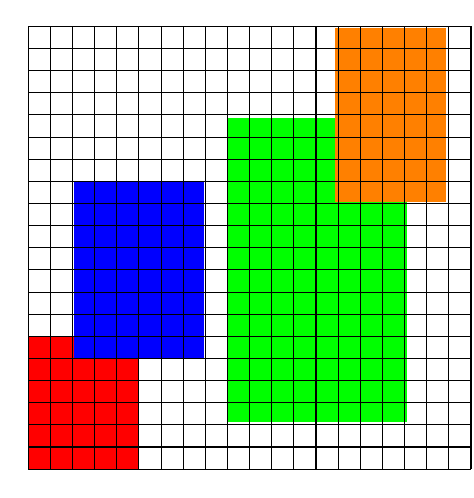
\begin{tikzpicture}(1,1)
  \draw [fill=red,red] (0,0) rectangle (1.39,1.68); 
  \draw [fill=blue,blue] (0.59,1.4) rectangle (2.23,3.65);
  \draw [fill=green,green] (2.55,0.6) rectangle (4.8,4.45);
  \draw [fill=orange,orange] (3.9,3.4) rectangle (5.3,5.6);
  \multiput(0, 0)(8, 0){21}{\line(0, 1){160}}
  \multiput(0, 0)(0, 8){21}{\line(1, 0){160}}
 \end{tikzpicture}
 \caption{5-colour image illustrating encoding redundancy}
 \label{COMP_ILLUS}
\end{figure}
\subsection{Predictive compression of KAT-7 data}
All compression techniques build on the central concept of reducing redundant data as pointed out previously. The exact definition of this redundancy is of course context 
dependent. In the case of the KAT-7 / MeerKAT array this redundancy may be defined in terms of the coherency of consecutive observations from each pair of dishes 
(or \textit{correlated} pairs). If the observations made are not particularly noisy it is reasonable to assume that the differences between consecutive values will be small.
Rather than storing each value it is possible to store the differences between observations (over a fixed time interval) instead. See figure~\ref{MeerKAT_PIPELINE}. 
The array observes a large spectrum of frequencies over a large number of correlated pairs, as indicated in the illustration. Each of these correlated frequency 
observations can be considered as steps of a time series. This report investigates how linear prediction can be employed to predict consecutive values for each of these time 
series. The goal is to minimise the difference between consecutive values, which can then be encoded using fewer bits than the original 32-bit sample size that is received 
by the processing and storage cluster. Such a scheme has the additional requirements of being \textit{lossless}, \textit{online} and fast.

\begin{figure}[h!]
 \centering
 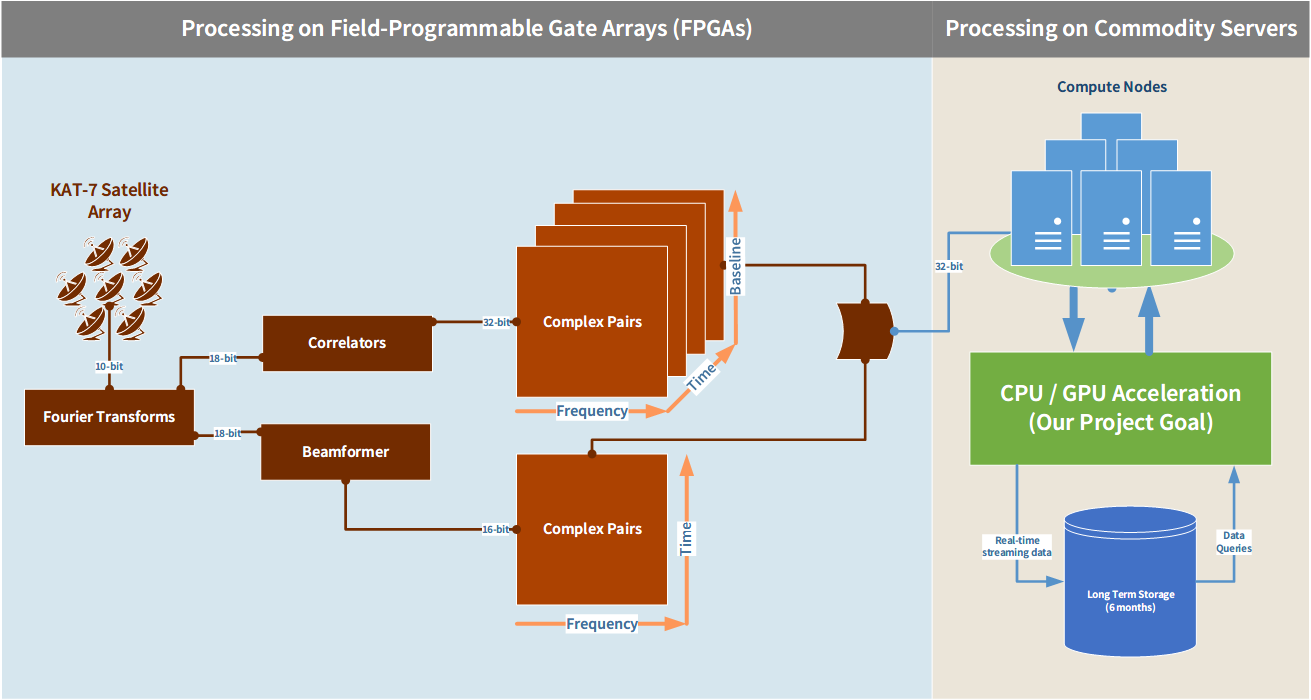
\includegraphics[width=0.8\textwidth]{Process.png}
 \caption{High-level overview of the MeerKAT pipeline}
 \label{MeerKAT_PIPELINE}
\end{figure}
\subsection{Compression algorithm properties and measurements}
In a lossless compression scheme the compression is completely invertible with \textit{no} loss of information after a decompression step is performed. Lossy
compression on the other hand discards unimportant data and gives much higher compression ratios than lossless methods. Lossy compression is useful in many
instances where subtle changes in data is not considered problematic. Some examples of this are the removal of high frequency data from images, sampling 
voice data at a lower rate than music or to employ a commonly used technique called \textit{quantization} where data is simply binned into consecutive ranges 
(or \textit{bins}).

An online compression scheme refers to a process of compressing data on-the-fly as it is being transmitted. The results are sent off to subsequent 
processes such transmission over a network or storage to disk. This is in contrast to to an offline scheme where data is compressed as a separate process which does not
form part of the primary work-flow of a system. An online process is normally required to be fast enough, as not to slow the overall data processing capabilities of 
a system.

Compression performance will be measured both in terms of effectiveness through a compression ratio described below \cite[p. 10]{salomon2004data} and throughput. A 
compression ratio closer to 0 indicates a smaller output file and values greater than 1 indicates that the algorithm inflated the data instead of shrinking it.
\begin{equation}
 \text{Compression ratio} := \frac{\text{size of the output stream}}{\text{size of the input stream}}
\end{equation}
\begin{equation}
 \text{Throughput} := \frac{\text{input processed (in GB)}}{\text{difference in time (in seconds)}}
\end{equation}
\subsection{Research questions}
Due to the limited scope of the project this report will only focus on evaluating algorithm performance and not algorithm integration into the KAT-7 / MeerKAT processing
pipeline. This research will include the construction of a parallel algorithm, as well as the investigation of the feasibility of porting this algorithm to the General 
Purpose Graphics Processing Unit (GPGPU)-accelerated nodes currently employed by the KAT-7 signal processing nodes as illustrated in figure~\ref{MeerKAT_PIPELINE}.

The algorithm will have to meet two primary criteria: high throughput and effective compression ratios. These are outlined below:
\begin{enumerate}
 \item Are predictive techniques fast enough? The algorithm should be able of achieving throughput rates of at least 40 GiB/s. These represent Infiniband network speeds 
 and represents a reasonable first milestone towards achieving compression at line rates.
 \item Are predictive techniques effective? The algorithm should reduce the size of transmissions by several percent and hopefully this reduction can take the form of 
       double digit figures. It has, however, been pointed out by the SKA office that the data may be too noisy to expect great reductions, while maintaining the throughput 
       rate mentioned above.
 \item Can throughput be traded for compression ratio using different predictors?
\end{enumerate}

Next a detailed breakdown of the most commonly used compression techniques is given. Thereafter a discussion will be given on a design of a predictive compression scheme, 
different implementation strategies, along with technical details, and a section with results and discussion.
\section{Background}
\subsection{Overview of data compression techniques}
There are considered to be 4 broad categories of compression techniques \cite{salomon2004data}. These are the basic methods, Lempel-Ziv methods, statistical methods 
and transforms.
\subsubsection{Basic methods}
The more intuitive methods include commonly employed methods such as Run-Length Encoding, which, simply put, encodes runs of characters using some reserved 
character and a number indicating the length of the run. In the context of compressing floating-point data such a scheme will focus on encoding runs of zeros and ones
at a bit level.

Another basic technique which is particularly relevant for application on numerical data is a predictive compression scheme. Such a compression scheme encodes the 
difference between each predicted succeeding value and the actual succeeding value as explained earlier. This can be quite successfully employed to compress data 
generated from time series \cite{engelson2000lossless}, but does rely on data coherence.
\subsubsection{Lempel-Ziv methods}
Lempel-Ziv is commonly referred to as “LZ” or dictionary methods, is a class of algorithms with many variants. It is one of the more popular \textit{adaptive} techniques 
in modern compression utilities. In their simplest form these methods normally use both a search- and lookahead buffer to encode recurrent phrases using fixed-size codes. An 
adaptive compression technique is useful in circumstances where the probability distribution of the underlying dataset is not known in advance or may change over time. 
One example of such an LZ method is used in the GNU compression utility Gzip. Gzip implements the DEFLATE algorithm which is a variant of the first LZ scheme, LZ-77 
\cite[ch. 3]{salomon2004data}.

LZ-77 encodes these recurrent phrases as length-distance pairs. If a sequence of characters are found to be the same as a sub-sequence of characters in the search buffer the 
distance to the start of that sub-sequence together with the length of the match is encoded. The size of the search buffer can be up to 32 kB in some implementations of the 
algorithm \cite[ch. 3]{salomon2004data}.
\subsubsection{Statistical methods}
This class of algorithms normally uses variable-length codes to achieve an optimal (or near optimal) encoding of dataset. In information theory this optimal encoding is 
described as an \textit{entropy} encoding. Entropy is the measurement of the information contained in a single base-n symbol (as transmitted per unit time by some source).

Redundancy is defined as the difference in entropy between the optimal encoding and the current encoding of a data set and is expressed in the following equation  
($n$ is the size of a symbol set and $P_{i}$ is the probability that a symbol $c_{i}$ is transmitted from a source)\cite[p. 46 - 47]{salomon2004data}:
\begin{equation}
 R := \log_2n + \sum_1^nP_i\log_2P_i
\end{equation}
As the name may suggest these techniques use the probability of occurrence of a value to assign shorter codes to frequently occurring values in order to eliminate redundancy. This 
class include two widely employed techniques known as Huffman and Arithmetic coding respectively. Huffman coding assigns shorter \textit{integral-length} codes, while arithmetic 
coding assigns \textit{real-length} subintervals of [0,1) to frequently occurring symbols \cite{Witten:1987:ACD:214762.214771}\cite[ch. 2]{salomon2004data}.

Huffman coding counts the number of occurrences of a particular symbol, sorts this list in ascending order and merges the rarest pairs of symbols into a single \textit{binary} 
(a tree in which each node can have up to 2 children) sub-tree and re-inserts the merged sub-tree into the list (still preserving the previously established order). The number of occurrences 
of each subtree will be the sum of occurrences of all the leaf nodes. Upon termination of this process only a single binary tree is left in the list. Each left-traversal adds a 0 to the encoding 
of a symbol, while each right-traversal adds a 1. When a leaf-node is reached the constructed encoding is an \textit{unambiguous} code for the symbol. Refer to figure~\ref{HUFFMAN} for an example.
In this case the symbol \textit{H} will be represented as 11 while some of the least frequent symbols such as \textit{B} will be represented by a longer code (0001 in this case).
\begin{figure}[h!]
 \centering
 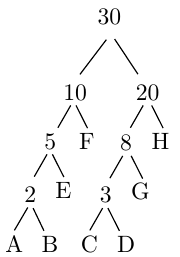
\includegraphics[width=0.15\textwidth]{huffmanTree.png}
 \caption{Sample of a completed Huffman-coding binary tree \cite[p. 70]{salomon2004data}}
 \label{HUFFMAN}
\end{figure}

Instead of assigning variable, \textit{integral}, length codes per symbol as is done by Huffman coding, Arithmetic coding encodes an entire message as a sub-interval of [0,1). As with
Huffman a probability distribution has to be determined (or be specified) before the algorithm can be executed. The initial interval [0,1) is reduced by each consecutive 
symbol. The length of the sub-interval is proportional to the probability of occurrence of the symbol being read. The final symbol gets assigned any value inside the remaining 
sub-interval. As the interval decreases the number of bits required to encode each consecutive interval increases. However, the average number of bits needed to store 
each symbol is closer to the that of the entropy encoding of the dataset, since this average number can be \textit{real} value, unlike that of the per-symbol encoding of Huffman \cite[ch. 2]{salomon2004data}.

Both approaches lead to variable-size codes. Both techniques have adaptive versions which are useful in situations where the probability distributions change or have to be estimated. 
This approach is also applicable to the situation where the symbol table has to be computed on the fly, because it is impossible to perform multiple passes over data. This can, for example
be the scenario when processing streaming data and all compression has to be completed on the fly. Arithmetic coding achieves higher compression ratios in both adaptive and non-adaptive cases 
when compared to Huffman coding. It should be pointed out that the decompression step of Arithmetic coding is slow and unsuitable for cases where fast access is 
required \cite{ray1995database,williams1999compressing}\cite[ch. 2]{salomon2004data}.

\subsubsection{Transforms}
As the name suggest it can be useful to transform a dataset from one form to another in order to exploit its features for the purposes of compression. Such transformations 
includes, for example, wavelet transforms. As the name suggests a wavelet is a small wave-like function that is only non-zero over a very small domain and is useful
to separate the low frequency components from the high frequency components of, for example, an image. JPEG2000 and DjVu are popular formats that use 
wavelet transforms. The dataset is generally sampled at increasing frequencies to produce a series of representations that gradually increases in resolution. When added together 
these representations will reconstruct the original dataset. A sample of the discrete cosine transform of an image (as employed by JPEG2000) is shown in figure~\ref{TRANSFORM_SAMPLE}. 
Only the transformation coefficients have to be stored in order to reconstruct each value in this series. The coefficients within this transformation can then be further compressed 
using other techniques, for example, Huffman coding and Run-Length Encoding (as is done in JPEG2000). If lossy compression (loss of accuracy which cannot be recovered after 
decompression) is tolerable, quantization can be used to discard unimportant values (for example the high frequency features of an image) \cite{952804}\cite[ch. 5]{salomon2004data}.
\begin{figure}[h!]
 \centering
 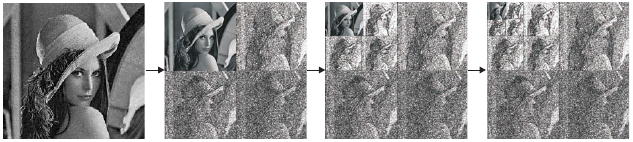
\includegraphics[width=1.0\textwidth]{DCTSample.png}
 \caption{Sample output from a Discrete Cosine Transform employed by JPEG2000 \cite{952804}}
 \label{TRANSFORM_SAMPLE}
\end{figure}

Transforms are furthermore particularly useful where multiple levels of detail are desired. An example of this may include the transfer of scientific data over a network 
for real-time analysis and observation. Low resolution samples can be consistently transferred, while higher resolution samples can be transferred upon request \cite{Tao:1994:PTS:951087.951108}.
\subsection{Overview of predictive compression}
Previous research \cite{1607248,4589203,engelson2000lossless,lindstrom2006fast,O'Neil:2011:FDC:1964179.1964189,4976448,CGF:CGF681} in this area has yielded good results both in terms of compression ratio and speed. 
The common line of thought is to predict successive values with reasonable precision. Depending on the accuracy of the prediction, the difference between the predicted and actual value will be much smaller than the actual value itself. 
This difference can then be encoded using fewer bytes/bits of data (depending if compression occurs at a byte or bit level) by compressing the leading zeros after either an XOR or integer subtraction 
operation. Machine instructions to count the leading zeros can be found on AMD and newer Intel Processors. The leading zero count is then encoded as a prefix stream while the remaining bits/bytes 
are encoded as a residual stream.

Previous research suggests several different constructions of predictors. The use of a \textit{Lorenzo} predictor \cite{lindstrom2006fast,CGF:CGF681} generalizes the well known parallelogram predictor. 
The Lorenzo predictor extends the parallelogram to arbitrary dimensions. More detail on the parallelogram predictor will be given
in the implementation section, but it is useful to note that this approach is particularly useful for compressing large meshes. Other approaches include the use of prediction history 
(via a simple lookup table construction) as suggested by Burtscher et al. \cite{1607248,4589203,4976448}. Burtscher et al. reports a throughput of up to 670 MB/s on a CPU implementation of their FPC 
compressor. An even simpler scheme by O'Neil et al. \cite{O'Neil:2011:FDC:1964179.1964189} reportedly achieved throughputs of up to 75GB/s for compression and up to 90GB/s 
decompression, implemented in CUDA. In this scheme only the difference between successive values are encoded (this will clearly only work if pairs of data points 
vary very little from one time step to the next). It is duly noted that the speeds achieved  are on the post-processing of results, already stored in graphics memory. 
The implementations by \cite{O'Neil:2011:FDC:1964179.1964189,1607248,4589203,4976448,engelson2000lossless} target 64-bit IEEE 754 
\textit{double} precision floating-point data.

The IEEE 754 standard of 2008 defines 3 interchange formats (32-bit, 64-bit and 128-bit). See figures~\ref{IEEE_FLOAT}~\&~\ref{IEEE_FLOAT_TAB}. Each of these have a common 
construction with the following subfields:
\begin{itemize}
 \item A 1-bit sign
 \item A w-bit length biased exponent
 \item A (d-1)-bit significand, where the leading bit of the significand is implicitly encoded in the exponent.
\end{itemize}
\begin{figure}[h!]
 \centering
 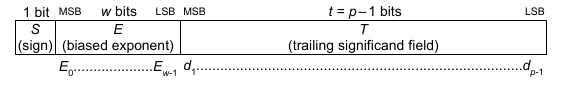
\includegraphics[width=0.6\textwidth]{IEEEinterchangeFormat.png}
 \caption{IEEE Interchange floating-point format \cite{4610935}}
 \label{IEEE_FLOAT}
\end{figure}
\begin{figure}[h!]
\centering
\begin{tabular}{|c|c|c|}
 \hline
 Precision & Exponent width & Significant precision \\
 \hline
 32-bit & 8 bits & 23 bits \\
 \hline
 64-bit & 11 bits & 52 bits \\
 \hline
\end{tabular}
\caption{Specifications for the 32-bit and 64-bit interchange formats}
 \label{IEEE_FLOAT_TAB}
\end{figure}
The primary scheme proposed in this paper takes its inspiration from the work of O'Neil et al. \cite{O'Neil:2011:FDC:1964179.1964189}, but will operate on 32-bit 
IEEE 754 \textit{single} precision floating-point values, as pointed out in the introduction. The uncompressed data itself is also structured slightly 
differently to the model used by O'Neil et al. \cite{O'Neil:2011:FDC:1964179.1964189}. Instead of compressing each consecutive value the proposed compressor will operate 
over consecutive time slices (refer to figure~\ref{MeerKAT_PIPELINE}).

As pointed out in previous research \cite{engelson2000lossless,lindstrom2006fast} using floating-point operations in the prediction step can cause an irreversible loss of information due to floating-point
rounding errors. A simple alternative approach is proposed by Engelson et al. \cite{engelson2000lossless}: floating-point memory is simply treated as integer memory and all operations performed on that memory are integer operations. This
approach ensures the predictive scheme achieves lossless compression. In light of this only schemes that conform to this approach will be considered. Engelson et al. \cite{engelson2000lossless} gives an example of how floating-point numbers
can be treated with integer operations. Figure~\ref{INT_REP} shows that if two floating-point numbers are relatively close to each other in terms of magnitude it is possible to discard some repeated bytes of information after performing 
an XOR operation to extract the remaining, seemingly random, residual bits. Therefore if an accurate prediction can be made for consecutive numbers a reasonable
saving in terms of compression ratio can be made.
\begin{figure}[h!]
\centering
\begin{tabular}{|c|c|c|c|}
 \hline
  & & byte & 1\hspace{8 pt}2\hspace{8 pt}3\hspace{8 pt}4\hspace{8 pt}5\hspace{8 pt}6\hspace{8 pt}7\hspace{8 pt}8\\
 \hline
 $a_{1}$ & 2.3667\textbf{1}76745585676 & $\Rightarrow$ & 40 02 ef \textbf{09 ad 18 c0 f6} \\
 \hline
 $a_{2}$ & 2.3667\textbf{2}76745585676 & $\Rightarrow$ & 40 02 ef \textbf{0e eb 46 23 2f} \\
 \hline
 $a_{3}$ & 2.3667\textbf{3}76745585676 & $\Rightarrow$ & 40 02 ef \textbf{14 29 73 85 6a} \\
 \hline
\end{tabular}
\caption{Treating 64-bit IEEE 754 double precision floating-points as integer memory \cite{engelson2000lossless}}
 \label{INT_REP}
\end{figure}
\section{Design and Methodology}
\subsection{Overview}
In light of the research questions and the limited scope of this report focus will be placed on the usefulness of a predictive data compression 
step in the context of the MeerKAT project. This will be limited to an investigation on whether the algorithm can operate at the desired line rate of
40 GiB/s and whether it provides reasonable compression ratios. This initial investigation precludes the implementation of the algorithm as part of 
the networking stack employed in the KAT-7 pipeline. Reasonable compression in this context means achieving compression ratios, comparable to industry standard 
tools like GZIP and BZIP2. The possibility of using alternative predictive schemes to trade some throughput for a better compression ratio will also be investigated.
Such alternative schemes will include the following (notes on their efficient implementation will be provided in the implementation section):
\begin{enumerate}
 \item A Lagrange polynomial extrapolation.
 \item A parallelogram predictor.
 \item Moving mean \& median predictors.
\end{enumerate}
The key success criteria for this investigation are the following:
\begin{enumerate}
 \item Throughput in excess of 40 GiB/s is achieved by both the compressor and decompressor.
 \item Effective compression ratios, comparable to those achieved by GZIP and BZIP2 are achieved.
\end{enumerate}
\subsection{Packing algorithm}
The compacting algorithm being proposed is based on the approach taken by O'Neil et al. \cite{O'Neil:2011:FDC:1964179.1964189}. The algorithm is almost \textit{symmetrical} in its compression and 
decompression stages. In this context symmetry means the algorithm is executed in the opposite direction when performing decompression. The primary difference is that the leading 
zero count does not have to be computed for each element being decompressed. Refer to figure~\ref{PACKING_ALGORITHM} for more details.
\begin{figure}[h!]
 \centering
 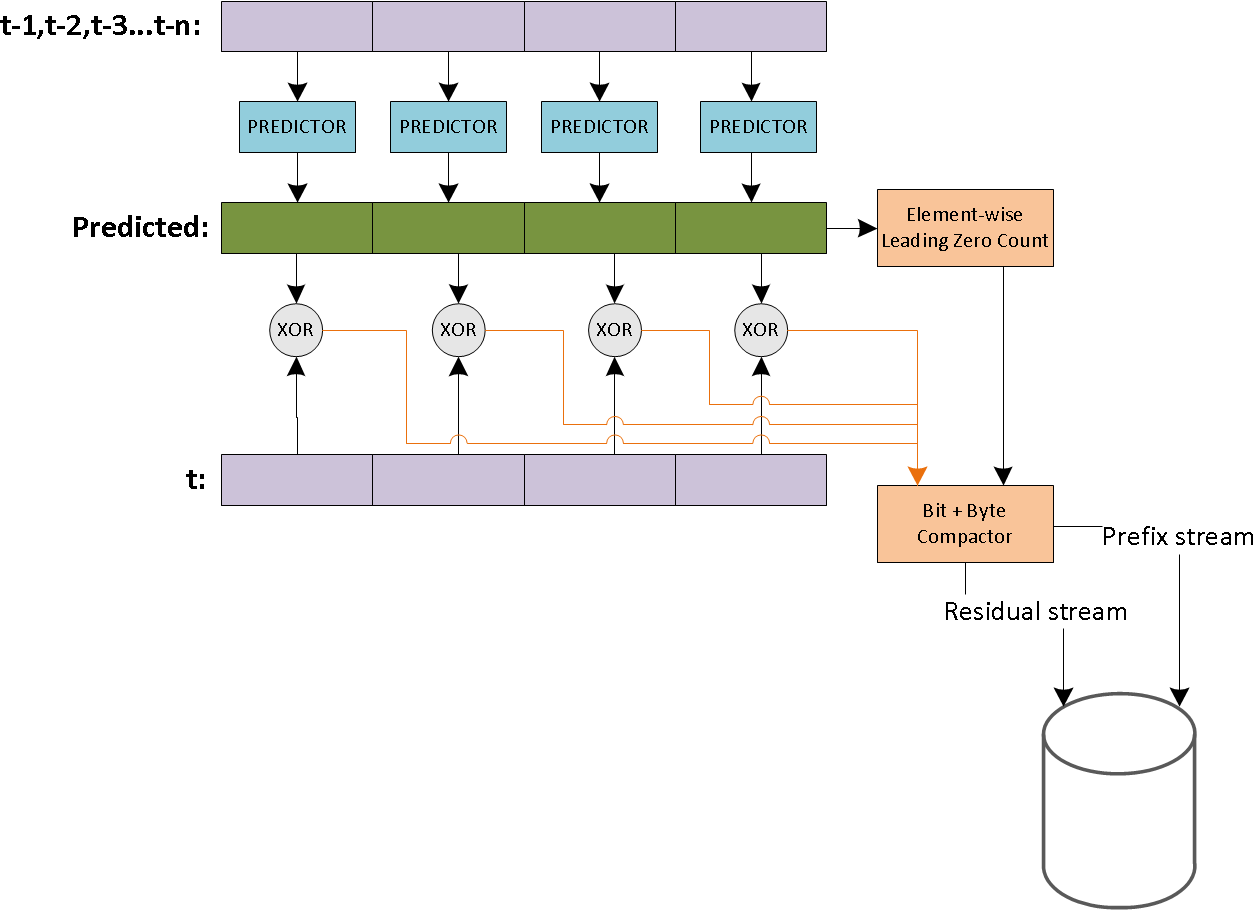
\includegraphics[width=0.7\textwidth]{Thesis_Alg.png}
 \caption{Prediction and compaction process}
 \label{PACKING_ALGORITHM}
\end{figure}
The construction of the algorithm being specified in figure~\ref{PACKING_ALGORITHM} is used because it allows for easy swapping between different predictors. The predictor in this case 
can be any n-element predictor. As mentioned earlier the predicted value is XORed with the actual value to get a residual which can be compacted at either bit or byte level. This 
compaction simply removes the leading zeros from each residual and stores each residual as a fixed-length prefix count. The number of bits needed to store $n$ leading 
zeros can be calculated as $\lfloor\log_2n\rfloor+1$ bits where $n\in\mathbb{N}_{>0}$. It remains to find the residual compaction scheme that gives the best results: packing at 
bit or byte level. Although a bit-packing scheme can pack an arbitrary number of zeros it requires longer prefixes to store the leading zero counts. The opposite is true 
for byte-packing schemes. Since the prefixes are always short a bit-packing scheme is used to store these fixed-length codes. Basic pseudo code is given in the implementation section.

Suppose the following two converted float values have to be compacted (the left-most byte is the most significant byte):
\begin{center}
  \begin{verbatim}
    #1: 00000000 01100010 01101000 11001001
    #2: 00000000 00000000 11110001 11110010
  \end{verbatim}
\end{center}
In this scenario the compaction of the residuals is done at byte level and the prefixes are done at bit level (assume 3 bits are needed to store up to 4 bytes of leading zeros):
\begin{center}
  \begin{verbatim}
    RESIDUALS:
    01100010 01101000 11001001 11110001 
    11110010
    PREFIXES (VALUES ARE PADDED UP TO ENSURE ONLY COMPLETE BYTES ARE STORED):
    00101000
  \end{verbatim}
\end{center} 
\subsection{Parallelizing compression and decompression steps}
There are three ways this can be achieved: 
\begin{enumerate}
 \item Even though the residuals are of variable length it is possible to pack them in parallel. However, there is an additional overhead to \textit{both} the packing and 
 unpacking process, since this approach requires a prefix sum to be computed for the array of element-wise leading zero counts as O'Neil et al. \cite{O'Neil:2011:FDC:1964179.1964189} 
 points out.
 
 A prefix sum (or \textit{scan}) can be defined on any binary associative operator, $\oplus$ over an ordered set with $I$ as its identity. If $A=[a_{0},a_{1},\dots,a_{n-1}]$ 
 is an ordered set then the prefix sum scan is defined as $scan(A):=[I,a_{0},(a_{0} \oplus a_{1}),\dots,(a_{0} \oplus a_{1} \oplus ... \oplus a_{n-2})]$. 
 
 In the context of the packing scheme proposed here, the prefix scan is defined over the normal integer addition operator. An example of this will be $scan[2,1,3,4] = [0,2,3,6]$ 
 under normal integer addition. The leading zero counts are saved to an array, \textit{A}, after which the scan operation is computed on the array. The accumulated values are 
 stored in place and hence the algorithm has a \textit{constant} memory overhead (uses no extra memory). Each index \textit{A}[\textit{i}] will therefore store the starting 
 position (in bits) of the residual of the $i^{th}$ element \cite{blelloch1990prefix}. 

 This scan operation can be computed in parallel. Blelloch suggests such an approach \cite{blelloch1990prefix}. The algorithm will be discussed in greater detail in the 
 implementation section. Additionally a work-efficient CUDA version of the algorithm is discussed in GPU Gems 3 \cite{harris2007parallel}. In this version the algorithm is 
 optimized to avoid \textit{bank conflicts} (see the section on GPU architecture) and has been shown to be up to 6 times faster than a sequential CPU implementation for large 
 arrays.
 
 After the indexes have been accumulated using the prefix sum algorithm it is easy to see how different threads can pack residuals at the correct positions. Both a bit and byte
 packing scheme will, however, require \textit{atomic} operations to ensure against the \textit{race condition} that arises when multiple threads write to the same memory 
 location simultaneously. This memory-level-synchronization mechanism adds additional overhead in terms of wasted machine clock cycles.
 \item Incoming data can also be separated into blocks, after which multiple of these blocks can be done in parallel (where each block is compressed/decompressed in serial). This overcomes the issue of 
 additional overheads arising due to computing prefix sums and using atomics. This approach may have a detrimental effect on the compression ratio since the length of the residual array of each block 
 has to be stored.
 \item A more fine-grained parallelization is possible using vectorized instructions. The various Intel SSE, Steaming SIMD (Single Instruction Multiple Data) instruction set extensions (up to version 4.2) provide
 the opportunity to perform 4 instructions (adds, multiplies, logarithms, rounding, etc.) simultaneously per core. However, the SSE instruction sets do not have any element-wise bit-shift operations. A combination 
 of the Intel SSE and AMD XOP instruction sets, will however, provide enough support to write the most of the algorithm using vector intrinsics. The XOP instruction set extends the SSE instruction set by adding these 
 operations as one of its primary features. Adding these instructions will, however, make the implementation dependent on the architecture of the underlying machine it is executed on (and therefore less portable). 
 If this approach is successful the vectorized code should be extended to use the latest Intel AVX 2 instruction set in which Intel introduces element-wise shift operations and offset-loading operations in future work. 
 The AVX family of instructions can compute up to 8 SIMD operations in parallel per core. All these vectorized instruction sets make use of a very limited number of 128- and 256-bit registers (SSE and AVX respectively).
 It remains to be investigated whether it is worthwhile to implement the proposed packing algorithm using SSE and XOP instructions.
\end{enumerate}
\subsection{Porting the implementation to CUDA}
General Purpose programming using Graphics Processing Units (GPGPU) brings a host of associated challenges. These challenges arise primarily due to the widely differing architecture of GPUs if compared
with the classical architectures of Central Processing Units (CPUs). Refer to figure~\ref{FERMI_ARCH} for a detailed overview of the microchip die structure of a Nvidia Fermi generation GPU. 
However, each generation of GPUs have widely differing architectures, each making many architecture specific optimizations. Each generation, for instance, will have both a 
different ratio and configuration of arithmetic cores to floating-point and special operations cores, per group of processing \textit{CUDA cores}. These cores are also known as 
\textit{SMs} (or \textit{SMXs} on the latest \textit{Kepler} generation). Additionally each generation has widely differing memory controller layouts. These may determine 
how many \textit{warps} of threads can be executed, when the warps are swapped in/out, along with many others. Each SM is split into atomic groups of threads which are executed
in parallel (normally this is specified as 32 threads per warp). Even if only a subset of these threads have work the entire warp will be executed on the same machine clock cycle.

A basic CUDA implementation will be provided to see if doing compression as a post-processing step on signal data already loaded to GPU (as part of the current pipeline) is a 
feasible alternative to a regular multi-threaded CPU implementation. Adaquite use of shared memory (as figure~\ref{FERMI_ARCH} shows GPUs have very large L1 and L2 caches available per SM) 
will be made and the implementation will take adequate precaution to \textit{coalesce} memory accesses and to avoid \textit{bank conflicts} when possible. 

Coalesced memory accesses are made if a continuous chunk of memory is accessed by a half-warp of threads at the same time. Normally these accesses have to be made in a uniform pattern. 
Individual memory calls to global graphics memory is a very costly operation (and therefore random accesses have to be avoided). Coalesced accesses are made simultaneously by the 
memory controller. Such accesses retrieve / write memory in larger chunks, which counters the latency associated with such an access. 

In GPU architectures (at the very least with Nvidia cards) \emph{shared} memory is divided up into banks. When multiple threads (specifically a half-warp of threads) try to 
access the same bank of memory, the memory accesses will be made sequentially. The general approach to avoid such a situation is to add padding between blocks of shared memory.

More details will be provided in the implementation section, but it is clear that a combination of the approaches (1 \& 2) taken with the CPU version will be required to make 
adequate use of the GPU architecture. This proposed implementation will consider assigning a block of data to each SM, which will in turn process that block in parallel without 
regard to operations performed on other SMs. This ensures that no unnecessary overheads due to costly card-wide synchronization steps are introduced. Instead all atomic 
operations and synchronization steps will be performed per-SM only.
\begin{figure}[h!]
 \centering
 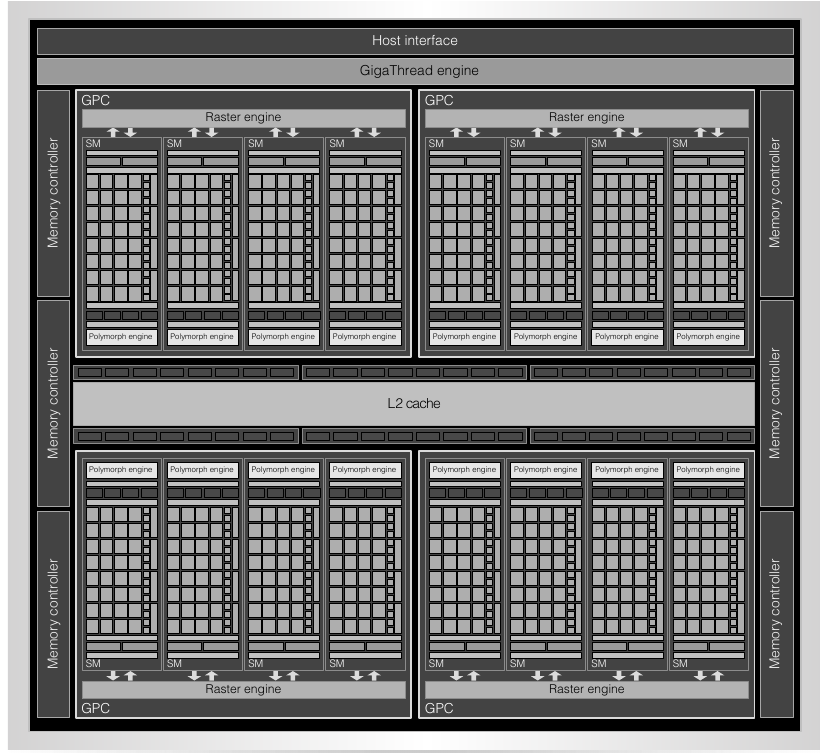
\includegraphics[width=0.8\textwidth]{fermi_arch.png}
 \caption{Architecture of the Fermi family of Nvidia GPUs \cite{wittenbrink2011fermi}}
 \label{FERMI_ARCH}
\end{figure}
\subsection{Test data}
The correlated data is provided in the form of HDF5 files. Each of these files stores a three dimensional array of complex pairs. The first dimension is time. The second 
is signal frequency (as mentioned in the background section the telescope array will monitor a wide range of frequencies). The third dimension is a combination of two 
properties. Each number represents a correlation between two antennae. The antennae additionally have two modes of polarization (a horizontal and vertical polarization). 
The size of the last dimension is specified as two times the number of permutations of $n + 1$: $2\times((n+1)\mathbf{P}2)$ elements where $n$ is the number of
antennae in the array. The headers of the HDF5 files contain meta-information on the state of the telescope and what it is currently observing (this will determine the 
characteristics of the data itself as well as the range of frequencies being monitored). 

It should be noted that the headers cannot be compressed with the algorithm being proposed. An LZ variant / entropy encoder may be better tailored for this task. 
The headers vary between 13-14\% of the total h5 file size. However, the data is only written to these formats after it is received by the processing cluster (see 
figure~\ref{MeerKAT_PIPELINE}). Therefore if the algorithm being proposed is integrated into the front end of the pipeline as seen in figure~\ref{MeerKAT_PIPELINE} (as part of 
future work) it may still provide a significant saving in network I/O. 
\subsection{Structure and scope of the benchmarks}
Some of these HDF5 files measure more than 30GB in size, each containing many timestamps, some spread over 4000 frequencies. It is reasonable to assume that once the number of correlations grow, emphasis will be placed on processing each 
time step (or portion thereof) as soon as it is received over the network. In future research the compressor may be integrated into the 7-layer OSI networking stack currently employed by the KAT-7 prototype. Due to the limited
scope of this project focus will be on analyzing the performance of the algorithms themselves and not to measure any disk I/O (except when comparing to other compression utilities for the sake of fairness).

This report will focus on the following analysis:
\begin{enumerate}
 \item A comparison between the a CPU implementation of the parallel (prefix sum-based algorithm) and the blocked approach (as specified previously) will be made.
 \item A detailed breakdown of how the algorithm performs on different numbers of cores (of whichever method is determined most fit in step 1) will be provided.
 \item The effectiveness of a parallelogram predictor, a Lagrange extrapolation predictor \cite{engelson2000lossless} and a moving mean and median scheme will be determined. 
       Each of these methods will be described in greater detail in the implementation chapter.
 \item The feasibility of implementation using the Intel SSE and AMD XOP vectorized instruction sets will be investigated.
 \item Benchmarks of the algorithm against the standard programs used for comparison: GZIP, BZIP2, ZIP and RAR. In this case the disk I/O will be included for the sake of fairness.
 \item The feasibility of a CUDA implementation, as outlined earlier will be determined.
 \item Finally results from concurrent research being conducted into entropy encoding and run-length encoding will be compared to those achieved in this investigation. This comparison will include a 
       breakdown of performance in terms of both throughput and compression ratios.
\end{enumerate}
\subsection{Benchmarking platform}
The benchmarking platform is designed with two primary software engineering goals in mind:
\begin{itemize}
 \item It should be as \textit{decoupled} as possible, making use of predefined interfaces. This will assist in providing several implementations of the CPU version (for example SSE, different linear predictors and different parallelization
 approaches) and simply swapping one implementation for another. Interactions between components must be kept to a minimum.
 \item The components must be \textit{cohesive}. They should contain only relevant operations and should be considered as atomic units.
\end{itemize}
The architecture described in figure~\ref{TOOL_ARCH} is used for the benchmarking platform. All the external dependencies depicted in the component model is freely available
and are actively maintained. There is no considerable technical risk in using these libraries. More detailed implementation details will be provided in the next section. The 
benchmark process is relatively simple and its flow is depicted in figure~\ref{TOOL_FLOW}.
\begin{figure}[h!]
 \centering
 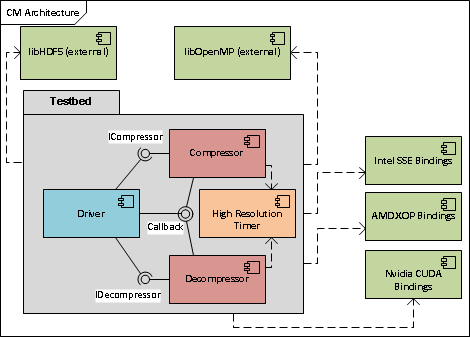
\includegraphics[width=0.6\textwidth]{Thesis_Arc.png}
 \caption{Architecture of the loosely coupled benchmarking platform, including external library dependencies}
 \label{TOOL_ARCH}
\end{figure}
\begin{figure}[h!]
 \centering
 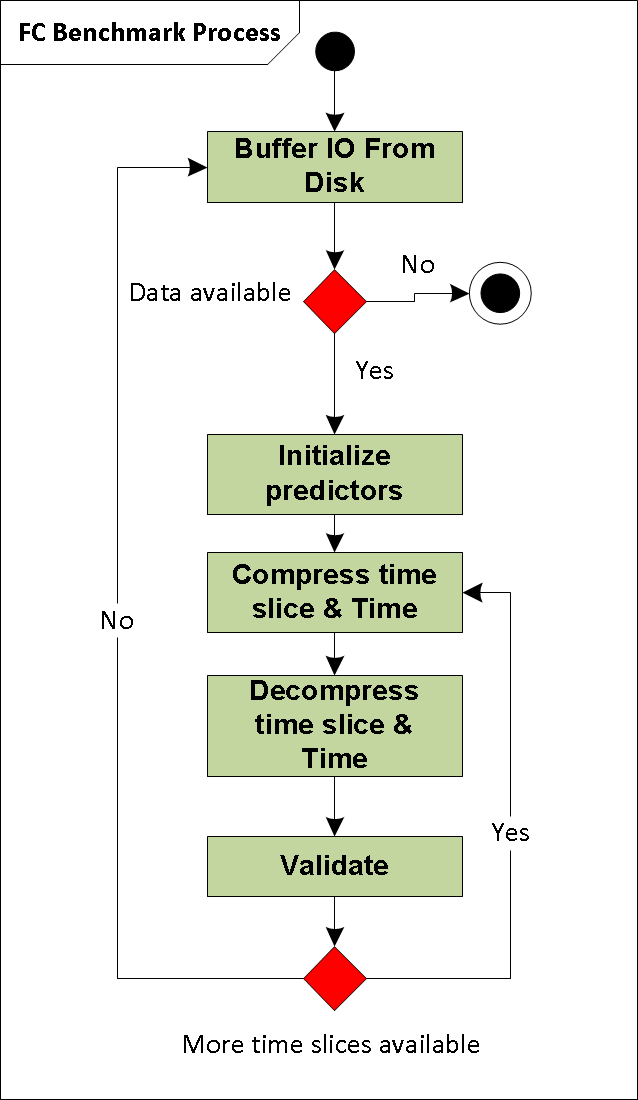
\includegraphics[width=0.25\textwidth]{Thesis_Flow.png}
 \caption{Behavioral model of the benchmarking platform}
 \label{TOOL_FLOW}
\end{figure}
\section{Implementation}
 \subsection{Basic algorithm}
  In order to give a more detailed description to the algorithm illustrated in figure~\ref{PACKING_ALGORITHM} in the previous section, the pseudo code for the compaction
  process is given below:
\begin{verbatim}
SUBROUTINE Compact(FLOAT[] data, UNSIGNED INT32 numElements, 
		    out UNSIGNED INT32[] residuals, 
		    out UNSIGNED INT32[] prefixes)
	 //ASSUMPTION: 3 BITS NEEDED TO STORE UP TO 4 BYTES OF LEADING ZEROS
	 //ASSUMPTION: COMPACTION IS DONE INTO 32 BIT INTEGER ARRAY
BEGIN
	 UNSIGNED INT32 bitPosInResidualArray = 0
	 FOR index = 0 TO numElements - 1 DO
		  /*
		  This prediction step requires up to "n" arrays of the 
		  same size of "data".
		  */
		  UNSIGNED INT32 predictedValue = linearPredict(index) 
		  UNSIGNED INT8 leadingZeroCount = clz(data[index])
		  UNSIGNED INT32 difference = predictedValue XOR data[index]
		  //save the prefix:
		  prefixes[index*3 INT_DIV 32] = SHIFT (leadingZeroCount INT_DIV 32) to \\
		    the index*3 MODULO 32 th bit
		  IF there are remaining bits that couldn't be fitted THEN
		    prefixes[index*3 INT_DIV 32 + 1] = SHIFT remaining bits that couldn't \\
		      be fitted in the previous operation to the first bit of the next byte
		  END IF
		  //save the residual:
		  residuals[bitPosInResidualArray INT_DIV 32] = SHIFT (difference to \\
		    the bitPosInResidualArray MODULO 32 th bit
		  IF there are remaining bits that couldn't be fitted THEN
		    residuals[bitPosInResidualArray INT_DIV 32 + 1] = SHIFT remaining bits \\
		      that couldn't be fitted in the previous operation to the first bit \\
		      of the next byte
		  END IF  
		  //increment position in the residual array
		  bitPosInResidualArray += leadingZeroCount INT_DIV 8
	 END FOR
END SUBROUTINE
\end{verbatim}
 \subsection{Alternative linear prediction schemes}
  The most basic prediction scheme simply encodes the difference between observations at time \textit{t} and $t+1$. This difference is given as $O[t]$ xor $O[t-1]$. This 
  scheme is sensitive to the structure of the underlying data. Such a scheme will only work if most consecutive values varies slowly over time. Using an n-element 
  predictor may help mitigate the effects of noise. However, as pointed out earlier: any operations over these n-elements have to be integer operations and not 
  floating point operations due to the rounding errors they may introduce (as pointed out in the background section). All floating-point memory are therefore cast to 
  integer-typed memory before values are retrieved.
  
  These predictions, however, still have to be fast and preferably have an average linear computational complexity, $\theta(n)$. The predictor will only 
  store the previous \textit{n} observations in a fixed-length queue. This implies that the memory overhead for the predictor is $nxm$ where m is the total 
  number of elements being processed at time $t$.
 \subsubsection{Lorenzo predictor}
 The n-dimensional Lorenzo predictor is a generalization of the two dimensional parallelogram predictor (see figure~\ref{LORENZO}). It can be used to predict scalar 
 functions that are polynomials of degree $n - 1$ and has been proven useful in scalar field compression \cite{CGF:CGF681}. In each of the 3 cases below only simple
 integer additions and subtractions are needed: the sum of the values in red are subtracted from the sum of the values in green. In the two dimensional case this 
 addition and subtraction is known as the \textit{parallelogram rule}. The predicted value is computed from previous observations as as $P = O[t-1] + O[t-2] - O[t-3]$.
  \begin{figure}[h!]
    \centering
    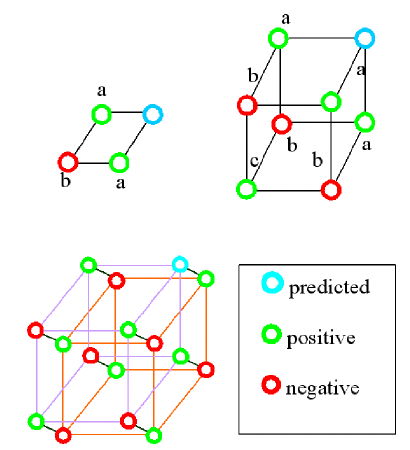
\includegraphics[width=0.3\textwidth]{lorenzo.png}
    \caption{Lorenzo predictor for 2D (upper left), 3D (upper right) and 4D (lower left) data \cite{CGF:CGF681}}
    \label{LORENZO}
  \end{figure} 
 \subsubsection{Moving average and moving mean}
  An integer-based moving mean is simple to implement and involves only a sumation and an integer division and therefore clearly has a linear computational complexity.
  However, the mean of a sample is sensitive to outliers, and therefore will not work well for noisy data. A simple solution will be to use a median based scheme
  where the predicted value is the center value of a \textit{sorted} list of observations. However, a naive implementation of such a median-based scheme will
  be slow due to the overheads of sorting. Wirth \cite{wirth76} suggests an algorithm to select the median using a basic \textit{pivoting} scheme in $\theta(n)$
  time. A pivot divides a dataset into two groups. The elements in the group to the right of the pivot is larger than the pivot and the elements in the group to
  the left of the pivot is smaller or equal to the pivot. The two groups do \emph{not} necessarily have to be ordered. The median is chosen through the following
  method that selects the \textit{k-th largest value} \cite{wirth76}:
  \begin{verbatim}
FUNCTION INT32 pivotMedian(INT32[] data, int n) {
    INT32 i, j, l, m, k = n/2-1 //k is the kth largest element in the array
    INT32 x, s

    l=0 //lower bound
    m=n-1 //upper bound
    WHILE l<m: //swap elements in group L and M until the two indexers cross
        x=data[k]
        i=l
        j=m
        REPEAT
	    //find 1 element in each sub-array that has to be swapped
	    //to the other sub-array:
            WHILE data[i]<x: i++
            WHILE x<data[j]: j--
            IF i<=j THEN
		    //swap:
                s=data[i]
                data[i]=data[j]
                data[j]=s
                i++
                j--
            END IF
        WHILE i<=j
        if(j<k) l=i
        if(k<i) m=j
    END WHILE
    RETURN data[k] //mid-point in the array
}
  \end{verbatim}
 \subsubsection{Lagrange prediction}
  {\color{red}TODO: Self.note.add also  include notes about the smoothness of data}
 \subsection{Algorithm parallelization}
  {\color{red}TODO}
 \subsection{SSE and XOP intrinsics} 
  {\color{red}TODO} 
 \subsection{GPGPU implementation in CUDA}
  {\color{red}TODO}
\section{Results}
\subsection{Constraints on benchmarking environment}
In order to eliminate the influence of the external testing environment the following special conditions are specified:
\begin{enumerate}
 \item Files in excess of 500 MB will be used for benchmarking. This will greatly reduce variability in timings.
 \item No other processes should be making intensive use of primary memory once benchmarking has commenced. The sheer quantity of data being processed makes benchmarking a memory-bound operation.
\end{enumerate}
\subsection{Parallelization approach}
\subsection{Performance of the block-based parallel scheme}
\subsection{Feasibility of including vector intrinsics}
\subsection{Benchmark against standard compression utilities}
\subsection{Feasibility of a CUDA implementation}
\subsection{Comparison to what was achieved in concurrent research}
\section{Discussion}
{\color{red}TODO}
\section{Conclusion}
{\color{red}TODO}
\section{Future avenues of research}
{\color{red}TODO}
\section{Glossary}
{\color{red}TODO}
\bibliographystyle{plain}
\bibliography{litRefs}
\end{document} to your LaTeX file where you want your
% title page.
%
%%%%%%%%%%%%%%%%%%%%%%%%%%%%%%%%%%%%%%%%%

%----------------------------------------------------------------------------------------
%	PACKAGES AND OTHER DOCUMENT CONFIGURATIONS
%----------------------------------------------------------------------------------------

\documentclass[12pt]{article}
\usepackage[utf8]{inputenc}
\usepackage{graphicx}
\usepackage{caption}
\usepackage{subcaption}
\usepackage{color}
\usepackage{amsmath}
\usepackage{amsfonts}
\usepackage[a4paper]{geometry}
\usepackage{fullpage}
\usepackage{parskip}
\usepackage{tikz}
\usepackage{hyperref}
\begin{document}

\begin{titlepage}

\newcommand{\HRule}{\rule{\linewidth}{0.5mm}} % Defines a new command for the horizontal lines, change thickness here

\center % Center everything on the page
 
%----------------------------------------------------------------------------------------
%	HEADING SECTIONS
%----------------------------------------------------------------------------------------

\textsc{\LARGE University of Cape Town}\\[1.5cm] % Name of your university/college
\textsc{\Large Department of Computer Science}\\[0.5cm] % Major heading such as course name
\textsc{\large CSC4000W - Honours in Computer Science}\\[0.5cm] % Minor heading such as course title

%----------------------------------------------------------------------------------------
%	TITLE SECTION
%----------------------------------------------------------------------------------------

\HRule \\[0.4cm]
{ \huge \bfseries Fast online predictive compression of radio astronomy data}\\[0.4cm] % Title of your document
\HRule \\[1.5cm]
 
%----------------------------------------------------------------------------------------
%	AUTHOR SECTION
%----------------------------------------------------------------------------------------

\begin{minipage}{0.4\textwidth}
\begin{flushleft} \large
\emph{Author:}\\
Benjamin \textsc{Hugo}\\ % Your name
\vspace{10pt}
\emph{Team members:}\\
Brandon \textsc{Talbot}\\ 
Heinrich \textsc{Strauss} 
\end{flushleft}
\end{minipage}
~
\begin{minipage}{0.4\textwidth}
\begin{flushright} \large
\emph{Supervisors:} \\
A/Prof. James \textsc{Gain}\\ % Supervisor's Name
Dr. Patrick \textsc{Marais}\\
\vspace{10pt}
\emph{External Advisor:} \\
Jason \textsc{Manley}
\end{flushright}
\end{minipage}\\[4cm]

% If you don't want a supervisor, uncomment the two lines below and remove the section above
%\Large \emph{Author:}\\
%John \textsc{Smith}\\[3cm] % Your name

%----------------------------------------------------------------------------------------
%	DATE SECTION
%----------------------------------------------------------------------------------------

{\large \today}\\[3cm] % Date, change the \today to a set date if you want to be precise

%----------------------------------------------------------------------------------------
%	LOGO SECTION
%----------------------------------------------------------------------------------------

%\includegraphics{Logo}\\[1cm] % Include a department/university logo - this will require the graphicx package
 
%----------------------------------------------------------------------------------------

\vfill % Fill the rest of the page with whitespace

\end{titlepage}

\begin{center} 
  {\LARGE Acknowledgements}
\end{center}
\vspace{50pt}

I would like to acknowledge A/Prof. James Gain and Dr. Patrick Marais of the Department of Computer Science at the University of Cape Town for their continuous, expert, input on the project.

Secondly I would like to thank Jason Manley, a Digital Signals Processing specialist at the MeerKAT offices in Pinelands, Cape Town for providing us with technical information
on the MeerKAT project. Jason has also kindly prepared a 100 GB of sample of KAT-7 output data for testing purposes.

Thirdly I would like to note that all tests were performed on the ICTS High Performance (\textit{HEX}) cluster at the University of Cape Town. The cluster has 4 DELL C6145 nodes each boasting 4 16-core
AMD Opteron 6274 CPUs, clocked at 2200 MHz with 16 MB L3 cache memory. There are two additional GPU nodes with 4 Tesla M2090 GPU cards each. Each GPU card has 6 GB GDDR5 and 2048 CUDA cores. I want to 
especially thank Andrew Lewis from ICTS for his assistance and support during testing.

This research is made possible under grant of the National Research Foundation (hereafter \textit{NRF}) of the Republic of South Africa. All views expressed in this report are those of the author and not 
necessarily those the NRF.
\pagebreak
\begin{abstract}
 {\color{red}TODO: add at end of writeup}
\end{abstract}
\pagebreak
\tableofcontents
\pagebreak
\section{Introduction}
\subsection{The KAT-7, MeerKAT and SKA}
South Africa and Australia are the two primary hosting countries for what is to become the largest radio telescope array in the world, known as the Square Kilometer Array (SKA). 
The SKA will give astronomers the opportunity to capture very high resolution images, over a wide field of view, covering a wide range of frequencies ranging 
from 70 MHz to 10 GHz. Upon completion in 2024 the array will consist of around 3000 dishes in the high frequency range and thousands of smaller antennae to 
cover the low frequency band. The South African branch of the SKA will be completed in 3 main phases. Phase 1 is a fully operational prototype 7-dish array 
called the KAT-7. The second phase, known as the MeerKAT, will consist of approximately 90 dishes. These are to be erected in the central Karoo region of South Africa. 
The final phase will add the remaining dishes and increase the baseline of the telescope to roughly 3000 km.

Due to the high signal sampling rate it is expected that each of these dishes will produce data rates of up to 420 GiB/s, while the lower frequency aperture arrays 
will produce up to 16 TiB/s. These rates, coupled with the scale of the SKA, will require a processing facility capable of handling as much as 1 Petabyte of 
data every 20 seconds, necessitating massive storage facilities. Innovative techniques are required to deal with the complex dual-requirement of high 
\textit{throughput rates} while effectively reducing the large storage requirements by means of \textit{data compression}. 
\subsection{Data compression \& decompression}
Data compression seek to encode data using a fewer number of bits than that of the original encoding. By removing such redundant data it is possible to effectively 
reduce the size of the dataset. A simple illustration of this can be found in figure~\ref{COMP_ILLUS}. It is clear that if this picture is stored naively as a 20x20
grid of 24-bit colours (8-bits for each of the red, green and blue channels) a lot of redundant data will be written to disk. A simple, yet effective, technique to 
reduce redundancy in this example is to store each horizontal line (or \textit{scanline}) of pixels as runs of colours, instead of individual colours. The first 
scanline can therefore be reduced to 9 white, 5 white, 5 orange, 1 white runs of pixels. This is known as \textit{Run-Length Encoding}. However, this is not the only 
form of redundancy: if each colour is represented as a 24-bit value, but only 5 colours are used from the $2^{24}$ colours available, a lot of storage space is wasted. 
In this case only  $\lfloor\log_{2}{5}\rfloor+1 = 4$ bits are needed to store all 5 colours uniquely. This variable-length encoding is often accomplished using a 
entropy encoding scheme which will be described to greater detail in the background section. Decompression can be thought of as the inverse operation to the compression 
process, which will reconstruct the original data from its encoded version.
\begin{figure}[ht!]
  \centering
 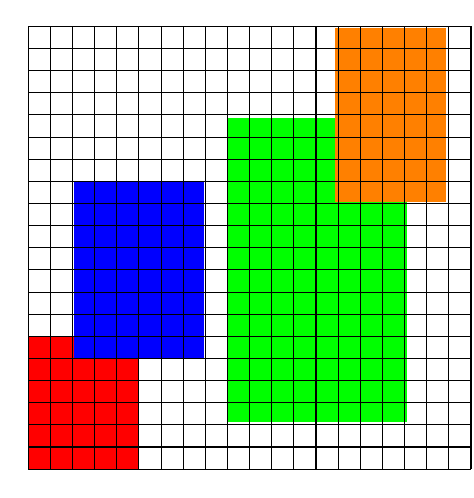
\begin{tikzpicture}(1,1)
  \draw [fill=red,red] (0,0) rectangle (1.39,1.68); 
  \draw [fill=blue,blue] (0.59,1.4) rectangle (2.23,3.65);
  \draw [fill=green,green] (2.55,0.6) rectangle (4.8,4.45);
  \draw [fill=orange,orange] (3.9,3.4) rectangle (5.3,5.6);
  \multiput(0, 0)(8, 0){21}{\line(0, 1){160}}
  \multiput(0, 0)(0, 8){21}{\line(1, 0){160}}
 \end{tikzpicture}
 \caption{5-colour image illustrating encoding redundancy}
 \label{COMP_ILLUS}
\end{figure}
\subsection{Predictive compression of KAT-7 data}
All compression techniques build on the central concept of reducing redundant data as pointed out previously. The exact definition of this redundancy is of course context 
dependent. In the case of the KAT-7 / MeerKAT array this redundancy may be defined in terms of the coherency of consecutive observations from each pair of dishes 
(or \textit{correlated} pairs). If the observations made are not particularly noisy it is reasonable to assume that the differences between consecutive values will be small.
Rather than storing each value it is possible to store the differences between observations (over a fixed time interval) instead. See figure~\ref{MeerKAT_PIPELINE}. 
The array observes a large spectrum of frequencies over a large number of correlated pairs, as indicated in the illustration. Each of these correlated frequency 
observations can be considered as steps of a time series. This report investigates how linear prediction can be employed to predict consecutive values for each of these time 
series. The goal is to minimise the difference between consecutive values, which can then be encoded using fewer bits than the original 32-bit sample size that is received 
by the processing and storage cluster. Such a scheme has the additional requirements of being \textit{lossless}, \textit{online} and fast.

\begin{figure}[h!]
 \centering
 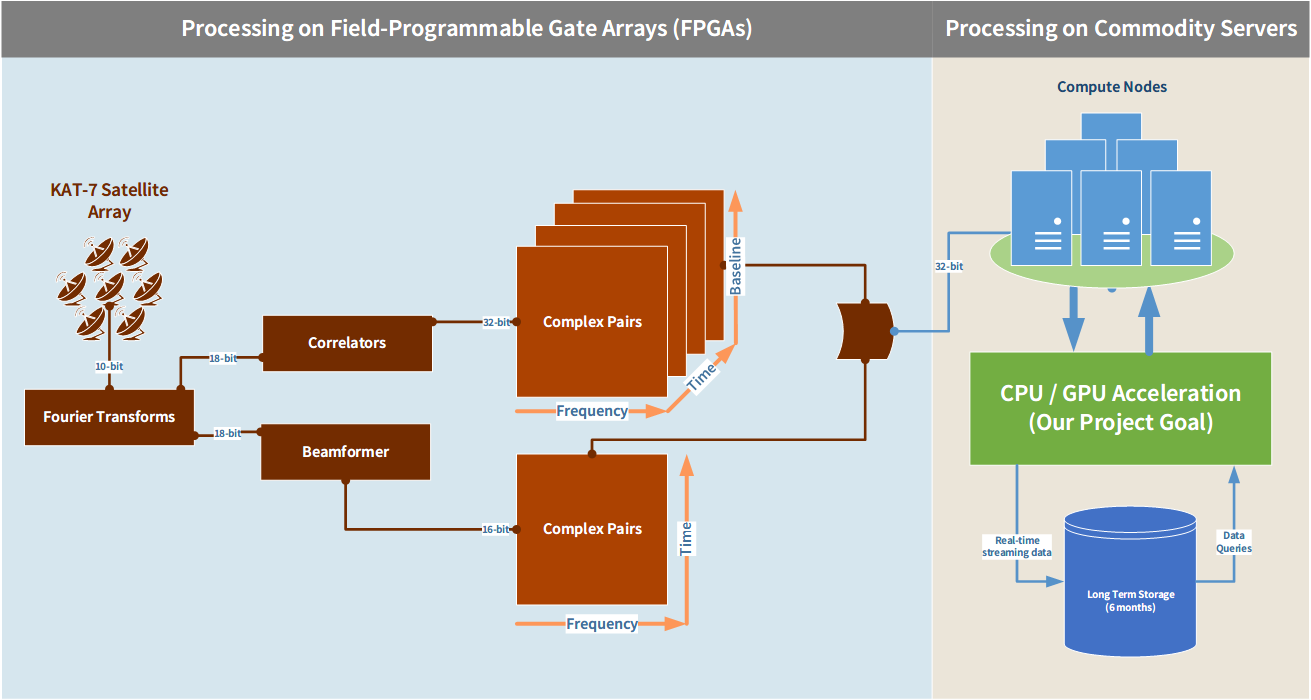
\includegraphics[width=0.8\textwidth]{Process.png}
 \caption{High-level overview of the MeerKAT pipeline}
 \label{MeerKAT_PIPELINE}
\end{figure}
\subsection{Compression algorithm properties and measurements}
In a lossless compression scheme the compression is completely invertible with \textit{no} loss of information after a decompression step is performed. Lossy
compression on the other hand discards unimportant data and gives much higher compression ratios than lossless methods. Lossy compression is useful in many
instances where subtle changes in data is not considered problematic. Some examples of this are the removal of high frequency data from images, sampling 
voice data at a lower rate than music or to employ a commonly used technique called \textit{quantization} where data is simply binned into consecutive ranges 
(or \textit{bins}).

An online compression scheme refers to a process of compressing data on-the-fly as it is being transmitted. The results are sent off to subsequent 
processes such transmission over a network or storage to disk. This is in contrast to to an offline scheme where data is compressed as a separate process which does not
form part of the primary work-flow of a system. An online process is normally required to be fast enough, as not to slow the overall data processing capabilities of 
a system.

Compression performance will be measured both in terms of effectiveness through a compression ratio described below \cite[p. 10]{salomon2004data} and throughput. A 
compression ratio closer to 0 indicates a smaller output file and values greater than 1 indicates that the algorithm inflated the data instead of shrinking it.
\begin{equation}
 \text{Compression ratio} := \frac{\text{size of the output stream}}{\text{size of the input stream}}
\end{equation}
\begin{equation}
 \text{Throughput} := \frac{\text{input processed (in GB)}}{\text{difference in time (in seconds)}}
\end{equation}
\subsection{Research questions}
Due to the limited scope of the project this report will only focus on evaluating algorithm performance and not algorithm integration into the KAT-7 / MeerKAT processing
pipeline. This research will include the construction of a parallel algorithm, as well as the investigation of the feasibility of porting this algorithm to the General 
Purpose Graphics Processing Unit (GPGPU)-accelerated nodes currently employed by the KAT-7 signal processing nodes as illustrated in figure~\ref{MeerKAT_PIPELINE}.

The algorithm will have to meet two primary criteria: high throughput and effective compression ratios. These are outlined below:
\begin{enumerate}
 \item Are predictive techniques fast enough? The algorithm should be able of achieving throughput rates of at least 40 GiB/s. These represent Infiniband network speeds 
 and represents a reasonable first milestone towards achieving compression at line rates.
 \item Are predictive techniques effective? The algorithm should reduce the size of transmissions by several percent and hopefully this reduction can take the form of 
       double digit figures. It has, however, been pointed out by the SKA office that the data may be too noisy to expect great reductions, while maintaining the throughput 
       rate mentioned above.
 \item Can throughput be traded for compression ratio using different predictors?
\end{enumerate}

Next a detailed breakdown of the most commonly used compression techniques is given. Thereafter a discussion will be given on a design of a predictive compression scheme, 
different implementation strategies, along with technical details, and a section with results and discussion.
\section{Background}
\subsection{Overview of data compression techniques}
There are considered to be 4 broad categories of compression techniques \cite{salomon2004data}. These are the basic methods, Lempel-Ziv methods, statistical methods 
and transforms.
\subsubsection{Basic methods}
The more intuitive methods include commonly employed methods such as Run-Length Encoding, which, simply put, encodes runs of characters using some reserved 
character and a number indicating the length of the run. In the context of compressing floating-point data such a scheme will focus on encoding runs of zeros and ones
at a bit level.

Another basic technique which is particularly relevant for application on numerical data is a predictive compression scheme. Such a compression scheme encodes the 
difference between each predicted succeeding value and the actual succeeding value as explained earlier. This can be quite successfully employed to compress data 
generated from time series \cite{engelson2000lossless}, but does rely on data coherence.
\subsubsection{Lempel-Ziv methods}
Lempel-Ziv is commonly referred to as “LZ” or dictionary methods, is a class of algorithms with many variants. It is one of the more popular \textit{adaptive} techniques 
in modern compression utilities. In their simplest form these methods normally use both a search- and lookahead buffer to encode recurrent phrases using fixed-size codes. An 
adaptive compression technique is useful in circumstances where the probability distribution of the underlying dataset is not known in advance or may change over time. 
One example of such an LZ method is used in the GNU compression utility Gzip. Gzip implements the DEFLATE algorithm which is a variant of the first LZ scheme, LZ-77 
\cite[ch. 3]{salomon2004data}.

LZ-77 encodes these recurrent phrases as length-distance pairs. If a sequence of characters are found to be the same as a sub-sequence of characters in the search buffer the 
distance to the start of that sub-sequence together with the length of the match is encoded. The size of the search buffer can be up to 32 kB in some implementations of the 
algorithm \cite[ch. 3]{salomon2004data}.
\subsubsection{Statistical methods}
This class of algorithms normally uses variable-length codes to achieve an optimal (or near optimal) encoding of dataset. In information theory this optimal encoding is 
described as an \textit{entropy} encoding. Entropy is the measurement of the information contained in a single base-n symbol (as transmitted per unit time by some source).

Redundancy is defined as the difference in entropy between the optimal encoding and the current encoding of a data set and is expressed in the following equation  
($n$ is the size of a symbol set and $P_{i}$ is the probability that a symbol $c_{i}$ is transmitted from a source)\cite[p. 46 - 47]{salomon2004data}:
\begin{equation}
 R := \log_2n + \sum_1^nP_i\log_2P_i
\end{equation}
As the name may suggest these techniques use the probability of occurrence of a value to assign shorter codes to frequently occurring values in order to eliminate redundancy. This 
class include two widely employed techniques known as Huffman and Arithmetic coding respectively. Huffman coding assigns shorter \textit{integral-length} codes, while arithmetic 
coding assigns \textit{real-length} subintervals of [0,1) to frequently occurring symbols \cite{Witten:1987:ACD:214762.214771}\cite[ch. 2]{salomon2004data}.

Huffman coding counts the number of occurrences of a particular symbol, sorts this list in ascending order and merges the rarest pairs of symbols into a single \textit{binary} 
(a tree in which each node can have up to 2 children) sub-tree and re-inserts the merged sub-tree into the list (still preserving the previously established order). The number of occurrences 
of each subtree will be the sum of occurrences of all the leaf nodes. Upon termination of this process only a single binary tree is left in the list. Each left-traversal adds a 0 to the encoding 
of a symbol, while each right-traversal adds a 1. When a leaf-node is reached the constructed encoding is an \textit{unambiguous} code for the symbol. Refer to figure~\ref{HUFFMAN} for an example.
In this case the symbol \textit{H} will be represented as 11 while some of the least frequent symbols such as \textit{B} will be represented by a longer code (0001 in this case).
\begin{figure}[h!]
 \centering
 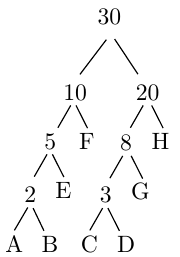
\includegraphics[width=0.15\textwidth]{huffmanTree.png}
 \caption{Sample of a completed Huffman-coding binary tree \cite[p. 70]{salomon2004data}}
 \label{HUFFMAN}
\end{figure}

Instead of assigning variable, \textit{integral}, length codes per symbol as is done by Huffman coding, Arithmetic coding encodes an entire message as a sub-interval of [0,1). As with
Huffman a probability distribution has to be determined (or be specified) before the algorithm can be executed. The initial interval [0,1) is reduced by each consecutive 
symbol. The length of the sub-interval is proportional to the probability of occurrence of the symbol being read. The final symbol gets assigned any value inside the remaining 
sub-interval. As the interval decreases the number of bits required to encode each consecutive interval increases. However, the average number of bits needed to store 
each symbol is closer to the that of the entropy encoding of the dataset, since this average number can be \textit{real} value, unlike that of the per-symbol encoding of Huffman \cite[ch. 2]{salomon2004data}.

Both approaches lead to variable-size codes. Both techniques have adaptive versions which are useful in situations where the probability distributions change or have to be estimated. 
This approach is also applicable to the situation where the symbol table has to be computed on the fly, because it is impossible to perform multiple passes over data. This can, for example
be the scenario when processing streaming data and all compression has to be completed on the fly. Arithmetic coding achieves higher compression ratios in both adaptive and non-adaptive cases 
when compared to Huffman coding. It should be pointed out that the decompression step of Arithmetic coding is slow and unsuitable for cases where fast access is 
required \cite{ray1995database,williams1999compressing}\cite[ch. 2]{salomon2004data}.

\subsubsection{Transforms}
As the name suggest it can be useful to transform a dataset from one form to another in order to exploit its features for the purposes of compression. Such transformations 
includes, for example, wavelet transforms. As the name suggests a wavelet is a small wave-like function that is only non-zero over a very small domain and is useful
to separate the low frequency components from the high frequency components of, for example, an image. JPEG2000 and DjVu are popular formats that use 
wavelet transforms. The dataset is generally sampled at increasing frequencies to produce a series of representations that gradually increases in resolution. When added together 
these representations will reconstruct the original dataset. A sample of the discrete cosine transform of an image (as employed by JPEG2000) is shown in figure~\ref{TRANSFORM_SAMPLE}. 
Only the transformation coefficients have to be stored in order to reconstruct each value in this series. The coefficients within this transformation can then be further compressed 
using other techniques, for example, Huffman coding and Run-Length Encoding (as is done in JPEG2000). If lossy compression (loss of accuracy which cannot be recovered after 
decompression) is tolerable, quantization can be used to discard unimportant values (for example the high frequency features of an image) \cite{952804}\cite[ch. 5]{salomon2004data}.
\begin{figure}[h!]
 \centering
 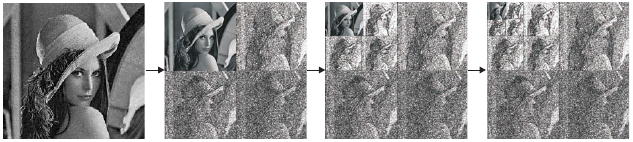
\includegraphics[width=1.0\textwidth]{DCTSample.png}
 \caption{Sample output from a Discrete Cosine Transform employed by JPEG2000 \cite{952804}}
 \label{TRANSFORM_SAMPLE}
\end{figure}

Transforms are furthermore particularly useful where multiple levels of detail are desired. An example of this may include the transfer of scientific data over a network 
for real-time analysis and observation. Low resolution samples can be consistently transferred, while higher resolution samples can be transferred upon request \cite{Tao:1994:PTS:951087.951108}.
\subsection{Overview of predictive compression}
Previous research \cite{1607248,4589203,engelson2000lossless,lindstrom2006fast,O'Neil:2011:FDC:1964179.1964189,4976448,CGF:CGF681} in this area has yielded good results both in terms of compression ratio and speed. 
The common line of thought is to predict successive values with reasonable precision. Depending on the accuracy of the prediction, the difference between the predicted and actual value will be much smaller than the actual value itself. 
This difference can then be encoded using fewer bytes/bits of data (depending if compression occurs at a byte or bit level) by compressing the leading zeros after either an XOR or integer subtraction 
operation. Machine instructions to count the leading zeros can be found on AMD and newer Intel Processors. The leading zero count is then encoded as a prefix stream while the remaining bits/bytes 
are encoded as a residual stream.

Previous research suggests several different constructions of predictors. The use of a \textit{Lorenzo} predictor \cite{lindstrom2006fast,CGF:CGF681} generalizes the well known parallelogram predictor. 
The Lorenzo predictor extends the parallelogram to arbitrary dimensions. More detail on the parallelogram predictor will be given
in the implementation section, but it is useful to note that this approach is particularly useful for compressing large meshes. Other approaches include the use of prediction history 
(via a simple lookup table construction) as suggested by Burtscher et al. \cite{1607248,4589203,4976448}. Burtscher et al. reports a throughput of up to 670 MB/s on a CPU implementation of their FPC 
compressor. An even simpler scheme by O'Neil et al. \cite{O'Neil:2011:FDC:1964179.1964189} reportedly achieved throughputs of up to 75GB/s for compression and up to 90GB/s 
decompression, implemented in CUDA. In this scheme only the difference between successive values are encoded (this will clearly only work if pairs of data points 
vary very little from one time step to the next). It is duly noted that the speeds achieved  are on the post-processing of results, already stored in graphics memory. 
The implementations by \cite{O'Neil:2011:FDC:1964179.1964189,1607248,4589203,4976448,engelson2000lossless} target 64-bit IEEE 754 
\textit{double} precision floating-point data.

The IEEE 754 standard of 2008 defines 3 interchange formats (32-bit, 64-bit and 128-bit). See figures~\ref{IEEE_FLOAT}~\&~\ref{IEEE_FLOAT_TAB}. Each of these have a common 
construction with the following subfields:
\begin{itemize}
 \item A 1-bit sign
 \item A w-bit length biased exponent
 \item A (d-1)-bit significand, where the leading bit of the significand is implicitly encoded in the exponent.
\end{itemize}
\begin{figure}[h!]
 \centering
 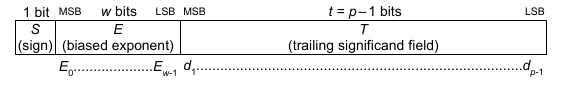
\includegraphics[width=0.6\textwidth]{IEEEinterchangeFormat.png}
 \caption{IEEE Interchange floating-point format \cite{4610935}}
 \label{IEEE_FLOAT}
\end{figure}
\begin{figure}[h!]
\centering
\begin{tabular}{|c|c|c|}
 \hline
 Precision & Exponent width & Significant precision \\
 \hline
 32-bit & 8 bits & 23 bits \\
 \hline
 64-bit & 11 bits & 52 bits \\
 \hline
\end{tabular}
\caption{Specifications for the 32-bit and 64-bit interchange formats}
 \label{IEEE_FLOAT_TAB}
\end{figure}
The primary scheme proposed in this paper takes its inspiration from the work of O'Neil et al. \cite{O'Neil:2011:FDC:1964179.1964189}, but will operate on 32-bit 
IEEE 754 \textit{single} precision floating-point values, as pointed out in the introduction. The uncompressed data itself is also structured slightly 
differently to the model used by O'Neil et al. \cite{O'Neil:2011:FDC:1964179.1964189}. Instead of compressing each consecutive value the proposed compressor will operate 
over consecutive time slices (refer to figure~\ref{MeerKAT_PIPELINE}).

As pointed out in previous research \cite{engelson2000lossless,lindstrom2006fast} using floating-point operations in the prediction step can cause an irreversible loss of information due to floating-point
rounding errors. A simple alternative approach is proposed by Engelson et al. \cite{engelson2000lossless}: floating-point memory is simply treated as integer memory and all operations performed on that memory are integer operations. This
approach ensures the predictive scheme achieves lossless compression. In light of this only schemes that conform to this approach will be considered. Engelson et al. \cite{engelson2000lossless} gives an example of how floating-point numbers
can be treated with integer operations. Figure~\ref{INT_REP} shows that if two floating-point numbers are relatively close to each other in terms of magnitude it is possible to discard some repeated bytes of information after performing 
an XOR operation to extract the remaining, seemingly random, residual bits. Therefore if an accurate prediction can be made for consecutive numbers a reasonable
saving in terms of compression ratio can be made.
\begin{figure}[h!]
\centering
\begin{tabular}{|c|c|c|c|}
 \hline
  & & byte & 1\hspace{8 pt}2\hspace{8 pt}3\hspace{8 pt}4\hspace{8 pt}5\hspace{8 pt}6\hspace{8 pt}7\hspace{8 pt}8\\
 \hline
 $a_{1}$ & 2.3667\textbf{1}76745585676 & $\Rightarrow$ & 40 02 ef \textbf{09 ad 18 c0 f6} \\
 \hline
 $a_{2}$ & 2.3667\textbf{2}76745585676 & $\Rightarrow$ & 40 02 ef \textbf{0e eb 46 23 2f} \\
 \hline
 $a_{3}$ & 2.3667\textbf{3}76745585676 & $\Rightarrow$ & 40 02 ef \textbf{14 29 73 85 6a} \\
 \hline
\end{tabular}
\caption{Treating 64-bit IEEE 754 double precision floating-points as integer memory \cite{engelson2000lossless}}
 \label{INT_REP}
\end{figure}
\section{Design and Methodology}
\subsection{Overview}
In light of the research questions and the limited scope of this report focus will be placed on the usefulness of a predictive data compression 
step in the context of the MeerKAT project. This will be limited to an investigation on whether the algorithm can operate at the desired line rate of
40 GiB/s and whether it provides reasonable compression ratios. This initial investigation precludes the implementation of the algorithm as part of 
the networking stack employed in the KAT-7 pipeline. Reasonable compression in this context means achieving compression ratios, comparable to industry standard 
tools like GZIP and BZIP2. The possibility of using alternative predictive schemes to trade some throughput for a better compression ratio will also be investigated.
Such alternative schemes will include the following (notes on their efficient implementation will be provided in the implementation section):
\begin{enumerate}
 \item A Lagrange polynomial extrapolation.
 \item A parallelogram predictor.
 \item Moving mean \& median predictors.
\end{enumerate}
The key success criteria for this investigation are the following:
\begin{enumerate}
 \item Throughput in excess of 40 GiB/s is achieved by both the compressor and decompressor.
 \item Effective compression ratios, comparable to those achieved by GZIP and BZIP2 are achieved.
\end{enumerate}
\subsection{Packing algorithm}
The compacting algorithm being proposed is based on the approach taken by O'Neil et al. \cite{O'Neil:2011:FDC:1964179.1964189}. The algorithm is almost \textit{symmetrical} in its compression and 
decompression stages. In this context symmetry means the algorithm is executed in the opposite direction when performing decompression. The primary difference is that the leading 
zero count does not have to be computed for each element being decompressed. Refer to figure~\ref{PACKING_ALGORITHM} for more details.
\begin{figure}[h!]
 \centering
 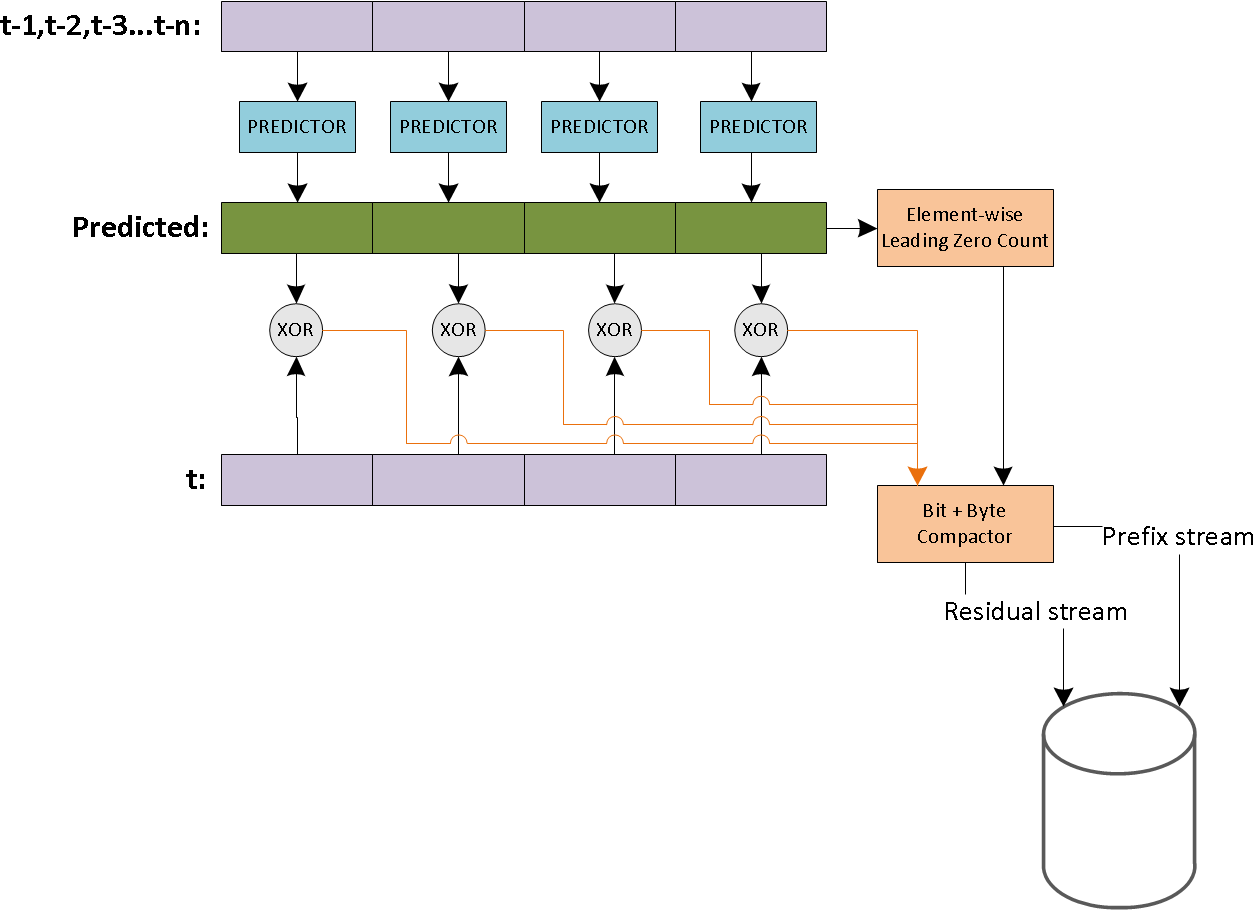
\includegraphics[width=0.7\textwidth]{Thesis_Alg.png}
 \caption{Prediction and compaction process}
 \label{PACKING_ALGORITHM}
\end{figure}
The construction of the algorithm being specified in figure~\ref{PACKING_ALGORITHM} is used because it allows for easy swapping between different predictors. The predictor in this case 
can be any n-element predictor. As mentioned earlier the predicted value is XORed with the actual value to get a residual which can be compacted at either bit or byte level. This 
compaction simply removes the leading zeros from each residual and stores each residual as a fixed-length prefix count. The number of bits needed to store $n$ leading 
zeros can be calculated as $\lfloor\log_2n\rfloor+1$ bits where $n\in\mathbb{N}_{>0}$. It remains to find the residual compaction scheme that gives the best results: packing at 
bit or byte level. Although a bit-packing scheme can pack an arbitrary number of zeros it requires longer prefixes to store the leading zero counts. The opposite is true 
for byte-packing schemes. Since the prefixes are always short a bit-packing scheme is used to store these fixed-length codes. Basic pseudo code is given in the implementation section.

Suppose the following two converted float values have to be compacted (the left-most byte is the most significant byte):
\begin{center}
  \begin{verbatim}
    #1: 00000000 01100010 01101000 11001001
    #2: 00000000 00000000 11110001 11110010
  \end{verbatim}
\end{center}
In this scenario the compaction of the residuals is done at byte level and the prefixes are done at bit level (assume 3 bits are needed to store up to 4 bytes of leading zeros):
\begin{center}
  \begin{verbatim}
    RESIDUALS:
    01100010 01101000 11001001 11110001 
    11110010
    PREFIXES (VALUES ARE PADDED UP TO ENSURE ONLY COMPLETE BYTES ARE STORED):
    00101000
  \end{verbatim}
\end{center} 
\subsection{Parallelizing compression and decompression steps}
There are three ways this can be achieved: 
\begin{enumerate}
 \item Even though the residuals are of variable length it is possible to pack them in parallel. However, there is an additional overhead to \textit{both} the packing and 
 unpacking process, since this approach requires a prefix sum to be computed for the array of element-wise leading zero counts as O'Neil et al. \cite{O'Neil:2011:FDC:1964179.1964189} 
 points out.
 
 A prefix sum (or \textit{scan}) can be defined on any binary associative operator, $\oplus$ over an ordered set with $I$ as its identity. If $A=[a_{0},a_{1},\dots,a_{n-1}]$ 
 is an ordered set then the prefix sum scan is defined as $scan(A):=[I,a_{0},(a_{0} \oplus a_{1}),\dots,(a_{0} \oplus a_{1} \oplus ... \oplus a_{n-2})]$. 
 
 In the context of the packing scheme proposed here, the prefix scan is defined over the normal integer addition operator. An example of this will be $scan[2,1,3,4] = [0,2,3,6]$ 
 under normal integer addition. The leading zero counts are saved to an array, \textit{A}, after which the scan operation is computed on the array. The accumulated values are 
 stored in place and hence the algorithm has a \textit{constant} memory overhead (uses no extra memory). Each index \textit{A}[\textit{i}] will therefore store the starting 
 position (in bits) of the residual of the $i^{th}$ element \cite{blelloch1990prefix}. 

 This scan operation can be computed in parallel. Blelloch suggests such an approach \cite{blelloch1990prefix}. The algorithm will be discussed in greater detail in the 
 implementation section. Additionally a work-efficient CUDA version of the algorithm is discussed in GPU Gems 3 \cite{harris2007parallel}. In this version the algorithm is 
 optimized to avoid \textit{bank conflicts} (see the section on GPU architecture) and has been shown to be up to 6 times faster than a sequential CPU implementation for large 
 arrays.
 
 After the indexes have been accumulated using the prefix sum algorithm it is easy to see how different threads can pack residuals at the correct positions. Both a bit and byte
 packing scheme will, however, require \textit{atomic} operations to ensure against the \textit{race condition} that arises when multiple threads write to the same memory 
 location simultaneously. This memory-level-synchronization mechanism adds additional overhead in terms of wasted machine clock cycles.
 \item Incoming data can also be separated into blocks, after which multiple of these blocks can be done in parallel (where each block is compressed/decompressed in serial). This overcomes the issue of 
 additional overheads arising due to computing prefix sums and using atomics. This approach may have a detrimental effect on the compression ratio since the length of the residual array of each block 
 has to be stored.
 \item A more fine-grained parallelization is possible using vectorized instructions. The various Intel SSE, Steaming SIMD (Single Instruction Multiple Data) instruction set extensions (up to version 4.2) provide
 the opportunity to perform 4 instructions (adds, multiplies, logarithms, rounding, etc.) simultaneously per core. However, the SSE instruction sets do not have any element-wise bit-shift operations. A combination 
 of the Intel SSE and AMD XOP instruction sets, will however, provide enough support to write the most of the algorithm using vector intrinsics. The XOP instruction set extends the SSE instruction set by adding these 
 operations as one of its primary features. Adding these instructions will, however, make the implementation dependent on the architecture of the underlying machine it is executed on (and therefore less portable). 
 If this approach is successful the vectorized code should be extended to use the latest Intel AVX 2 instruction set in which Intel introduces element-wise shift operations and offset-loading operations in future work. 
 The AVX family of instructions can compute up to 8 SIMD operations in parallel per core. All these vectorized instruction sets make use of a very limited number of 128- and 256-bit registers (SSE and AVX respectively).
 It remains to be investigated whether it is worthwhile to implement the proposed packing algorithm using SSE and XOP instructions.
\end{enumerate}
\subsection{Porting the implementation to CUDA}
General Purpose programming using Graphics Processing Units (GPGPU) brings a host of associated challenges. These challenges arise primarily due to the widely differing architecture of GPUs if compared
with the classical architectures of Central Processing Units (CPUs). Refer to figure~\ref{FERMI_ARCH} for a detailed overview of the microchip die structure of a Nvidia Fermi generation GPU. 
However, each generation of GPUs have widely differing architectures, each making many architecture specific optimizations. Each generation, for instance, will have both a 
different ratio and configuration of arithmetic cores to floating-point and special operations cores, per group of processing \textit{CUDA cores}. These cores are also known as 
\textit{SMs} (or \textit{SMXs} on the latest \textit{Kepler} generation). Additionally each generation has widely differing memory controller layouts. These may determine 
how many \textit{warps} of threads can be executed, when the warps are swapped in/out, along with many others. Each SM is split into atomic groups of threads which are executed
in parallel (normally this is specified as 32 threads per warp). Even if only a subset of these threads have work the entire warp will be executed on the same machine clock cycle.

A basic CUDA implementation will be provided to see if doing compression as a post-processing step on signal data already loaded to GPU (as part of the current pipeline) is a 
feasible alternative to a regular multi-threaded CPU implementation. Adaquite use of shared memory (as figure~\ref{FERMI_ARCH} shows GPUs have very large L1 and L2 caches available per SM) 
will be made and the implementation will take adequate precaution to \textit{coalesce} memory accesses and to avoid \textit{bank conflicts} when possible. 

Coalesced memory accesses are made if a continuous chunk of memory is accessed by a half-warp of threads at the same time. Normally these accesses have to be made in a uniform pattern. 
Individual memory calls to global graphics memory is a very costly operation (and therefore random accesses have to be avoided). Coalesced accesses are made simultaneously by the 
memory controller. Such accesses retrieve / write memory in larger chunks, which counters the latency associated with such an access. 

In GPU architectures (at the very least with Nvidia cards) \emph{shared} memory is divided up into banks. When multiple threads (specifically a half-warp of threads) try to 
access the same bank of memory, the memory accesses will be made sequentially. The general approach to avoid such a situation is to add padding between blocks of shared memory.

More details will be provided in the implementation section, but it is clear that a combination of the approaches (1 \& 2) taken with the CPU version will be required to make 
adequate use of the GPU architecture. This proposed implementation will consider assigning a block of data to each SM, which will in turn process that block in parallel without 
regard to operations performed on other SMs. This ensures that no unnecessary overheads due to costly card-wide synchronization steps are introduced. Instead all atomic 
operations and synchronization steps will be performed per-SM only.
\begin{figure}[h!]
 \centering
 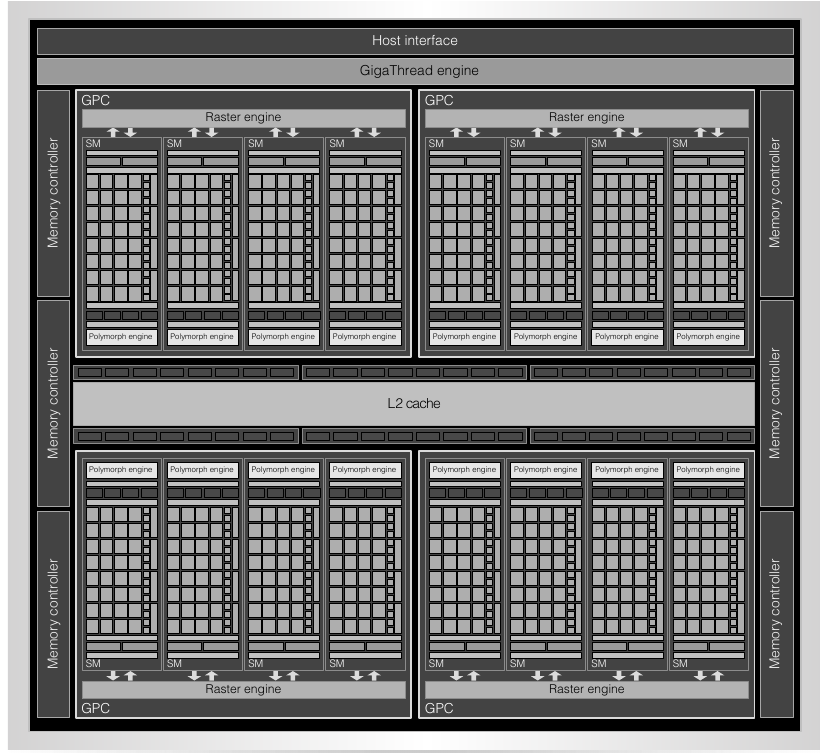
\includegraphics[width=0.8\textwidth]{fermi_arch.png}
 \caption{Architecture of the Fermi family of Nvidia GPUs \cite{wittenbrink2011fermi}}
 \label{FERMI_ARCH}
\end{figure}
\subsection{Test data}
The correlated data is provided in the form of HDF5 files. Each of these files stores a three dimensional array of complex pairs. The first dimension is time. The second 
is signal frequency (as mentioned in the background section the telescope array will monitor a wide range of frequencies). The third dimension is a combination of two 
properties. Each number represents a correlation between two antennae. The antennae additionally have two modes of polarization (a horizontal and vertical polarization). 
The size of the last dimension is specified as two times the number of permutations of $n + 1$: $2\times((n+1)\mathbf{P}2)$ elements where $n$ is the number of
antennae in the array. The headers of the HDF5 files contain meta-information on the state of the telescope and what it is currently observing (this will determine the 
characteristics of the data itself as well as the range of frequencies being monitored). 

It should be noted that the headers cannot be compressed with the algorithm being proposed. An LZ variant / entropy encoder may be better tailored for this task. 
The headers vary between 13-14\% of the total h5 file size. However, the data is only written to these formats after it is received by the processing cluster (see 
figure~\ref{MeerKAT_PIPELINE}). Therefore if the algorithm being proposed is integrated into the front end of the pipeline as seen in figure~\ref{MeerKAT_PIPELINE} (as part of 
future work) it may still provide a significant saving in network I/O. 
\subsection{Structure and scope of the benchmarks}
Some of these HDF5 files measure more than 30GB in size, each containing many timestamps, some spread over 4000 frequencies. It is reasonable to assume that once the number of correlations grow, emphasis will be placed on processing each 
time step (or portion thereof) as soon as it is received over the network. In future research the compressor may be integrated into the 7-layer OSI networking stack currently employed by the KAT-7 prototype. Due to the limited
scope of this project focus will be on analyzing the performance of the algorithms themselves and not to measure any disk I/O (except when comparing to other compression utilities for the sake of fairness).

This report will focus on the following analysis:
\begin{enumerate}
 \item A comparison between the a CPU implementation of the parallel (prefix sum-based algorithm) and the blocked approach (as specified previously) will be made.
 \item A detailed breakdown of how the algorithm performs on different numbers of cores (of whichever method is determined most fit in step 1) will be provided.
 \item The effectiveness of a parallelogram predictor, a Lagrange extrapolation predictor \cite{engelson2000lossless} and a moving mean and median scheme will be determined. 
       Each of these methods will be described in greater detail in the implementation chapter.
 \item The feasibility of implementation using the Intel SSE and AMD XOP vectorized instruction sets will be investigated.
 \item Benchmarks of the algorithm against the standard programs used for comparison: GZIP, BZIP2, ZIP and RAR. In this case the disk I/O will be included for the sake of fairness.
 \item The feasibility of a CUDA implementation, as outlined earlier will be determined.
 \item Finally results from concurrent research being conducted into entropy encoding and run-length encoding will be compared to those achieved in this investigation. This comparison will include a 
       breakdown of performance in terms of both throughput and compression ratios.
\end{enumerate}
\subsection{Benchmarking platform}
The benchmarking platform is designed with two primary software engineering goals in mind:
\begin{itemize}
 \item It should be as \textit{decoupled} as possible, making use of predefined interfaces. This will assist in providing several implementations of the CPU version (for example SSE, different linear predictors and different parallelization
 approaches) and simply swapping one implementation for another. Interactions between components must be kept to a minimum.
 \item The components must be \textit{cohesive}. They should contain only relevant operations and should be considered as atomic units.
\end{itemize}
The architecture described in figure~\ref{TOOL_ARCH} is used for the benchmarking platform. All the external dependencies depicted in the component model is freely available
and are actively maintained. There is no considerable technical risk in using these libraries. More detailed implementation details will be provided in the next section. The 
benchmark process is relatively simple and its flow is depicted in figure~\ref{TOOL_FLOW}.
\begin{figure}[h!]
 \centering
 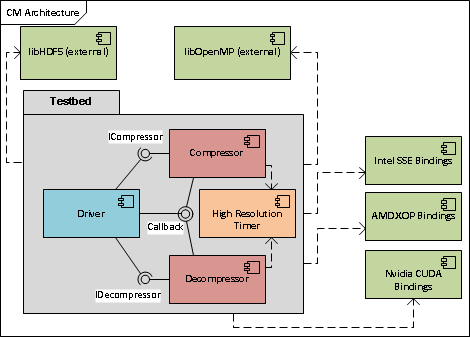
\includegraphics[width=0.6\textwidth]{Thesis_Arc.png}
 \caption{Architecture of the loosely coupled benchmarking platform, including external library dependencies}
 \label{TOOL_ARCH}
\end{figure}
\begin{figure}[h!]
 \centering
 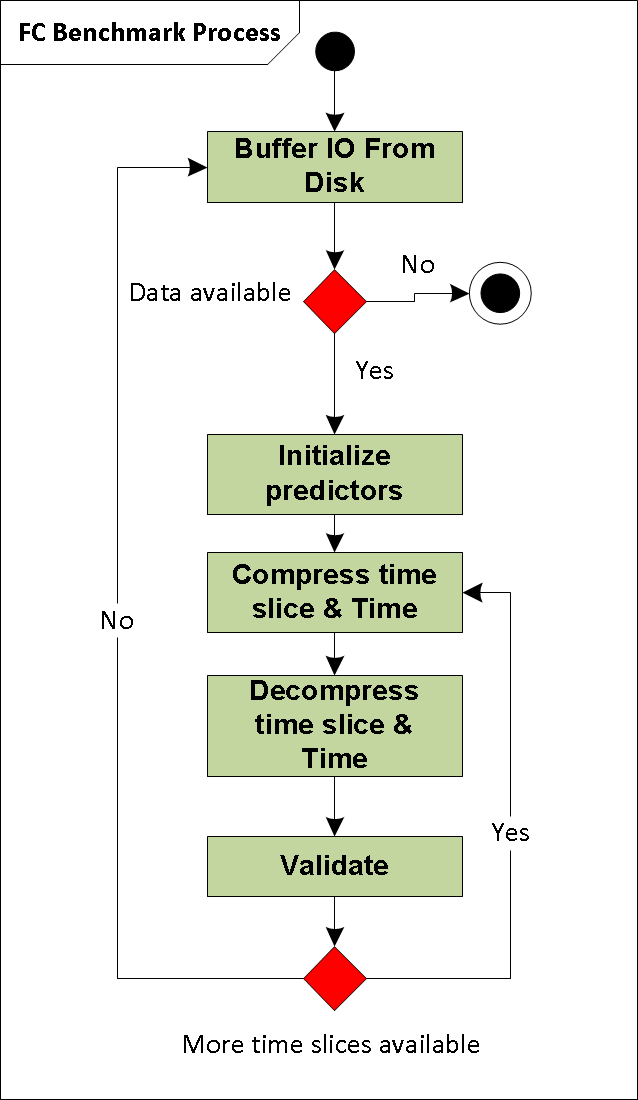
\includegraphics[width=0.25\textwidth]{Thesis_Flow.png}
 \caption{Behavioral model of the benchmarking platform}
 \label{TOOL_FLOW}
\end{figure}
\section{Implementation}
 \subsection{Basic algorithm}
  In order to give a more detailed description to the algorithm illustrated in figure~\ref{PACKING_ALGORITHM} in the previous section, the pseudo code for the compaction
  process is given below:
\begin{verbatim}
SUBROUTINE Compact(FLOAT[] data, UNSIGNED INT32 numElements, 
		    out UNSIGNED INT32[] residuals, 
		    out UNSIGNED INT32[] prefixes)
	 //ASSUMPTION: 3 BITS NEEDED TO STORE UP TO 4 BYTES OF LEADING ZEROS
	 //ASSUMPTION: COMPACTION IS DONE INTO 32 BIT INTEGER ARRAY
BEGIN
	 UNSIGNED INT32 bitPosInResidualArray = 0
	 FOR index = 0 TO numElements - 1 DO
		  /*
		  This prediction step requires up to "n" arrays of the 
		  same size of "data".
		  */
		  UNSIGNED INT32 predictedValue = linearPredict(index) 
		  UNSIGNED INT8 leadingZeroCount = clz(data[index])
		  UNSIGNED INT32 difference = predictedValue XOR data[index]
		  //save the prefix:
		  prefixes[index*3 INT_DIV 32] = SHIFT (leadingZeroCount INT_DIV 32) to \\
		    the index*3 MODULO 32 th bit
		  IF there are remaining bits that couldn't be fitted THEN
		    prefixes[index*3 INT_DIV 32 + 1] = SHIFT remaining bits that couldn't \\
		      be fitted in the previous operation to the first bit of the next byte
		  END IF
		  //save the residual:
		  residuals[bitPosInResidualArray INT_DIV 32] = SHIFT (difference to \\
		    the bitPosInResidualArray MODULO 32 th bit
		  IF there are remaining bits that couldn't be fitted THEN
		    residuals[bitPosInResidualArray INT_DIV 32 + 1] = SHIFT remaining bits \\
		      that couldn't be fitted in the previous operation to the first bit \\
		      of the next byte
		  END IF  
		  //increment position in the residual array
		  bitPosInResidualArray += leadingZeroCount INT_DIV 8
	 END FOR
END SUBROUTINE
\end{verbatim}
 \subsection{Alternative linear prediction schemes}
  The most basic prediction scheme simply encodes the difference between observations at time \textit{t} and $t+1$. This difference is given as $O[t]$ xor $O[t-1]$. This 
  scheme is sensitive to the structure of the underlying data. Such a scheme will only work if most consecutive values varies slowly over time. Using an n-element 
  predictor may help mitigate the effects of noise. However, as pointed out earlier: any operations over these n-elements have to be integer operations and not 
  floating point operations due to the rounding errors they may introduce (as pointed out in the background section). All floating-point memory are therefore cast to 
  integer-typed memory before values are retrieved.
  
  These predictions, however, still have to be fast and preferably have an average linear computational complexity, $\theta(n)$. The predictor will only 
  store the previous \textit{n} observations in a fixed-length queue. This implies that the memory overhead for the predictor is $nxm$ where m is the total 
  number of elements being processed at time $t$.
 \subsubsection{Lorenzo predictor}
 The n-dimensional Lorenzo predictor is a generalization of the two dimensional parallelogram predictor (see figure~\ref{LORENZO}). It can be used to predict scalar 
 functions that are polynomials of degree $n - 1$ and has been proven useful in scalar field compression \cite{CGF:CGF681}. In each of the 3 cases below only simple
 integer additions and subtractions are needed: the sum of the values in red are subtracted from the sum of the values in green. In the two dimensional case this 
 addition and subtraction is known as the \textit{parallelogram rule}. The predicted value is computed from previous observations as as $P = O[t-1] + O[t-2] - O[t-3]$.
  \begin{figure}[h!]
    \centering
    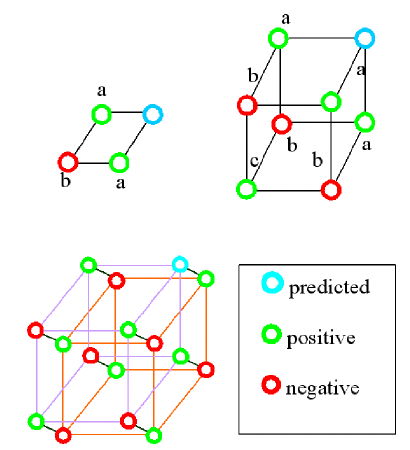
\includegraphics[width=0.3\textwidth]{lorenzo.png}
    \caption{Lorenzo predictor for 2D (upper left), 3D (upper right) and 4D (lower left) data \cite{CGF:CGF681}}
    \label{LORENZO}
  \end{figure} 
 \subsubsection{Moving average and moving mean}
  An integer-based moving mean is simple to implement and involves only a sumation and an integer division and therefore clearly has a linear computational complexity.
  However, the mean of a sample is sensitive to outliers, and therefore will not work well for noisy data. A simple solution will be to use a median based scheme
  where the predicted value is the center value of a \textit{sorted} list of observations. However, a naive implementation of such a median-based scheme will
  be slow due to the overheads of sorting. Wirth \cite{wirth76} suggests an algorithm to select the median using a basic \textit{pivoting} scheme in $\theta(n)$
  time. A pivot divides a dataset into two groups. The elements in the group to the right of the pivot is larger than the pivot and the elements in the group to
  the left of the pivot is smaller or equal to the pivot. The two groups do \emph{not} necessarily have to be ordered. The median is chosen through the following
  method that selects the \textit{k-th largest value} \cite{wirth76}:
  \begin{verbatim}
FUNCTION INT32 pivotMedian(INT32[] data, int n) {
    INT32 i, j, l, m, k = n/2-1 //k is the kth largest element in the array
    INT32 x, s

    l=0 //lower bound
    m=n-1 //upper bound
    WHILE l<m: //swap elements in group L and M until the two indexers cross
        x=data[k]
        i=l
        j=m
        REPEAT
	    //find 1 element in each sub-array that has to be swapped
	    //to the other sub-array:
            WHILE data[i]<x: i++
            WHILE x<data[j]: j--
            IF i<=j THEN
		    //swap:
                s=data[i]
                data[i]=data[j]
                data[j]=s
                i++
                j--
            END IF
        WHILE i<=j
        if(j<k) l=i
        if(k<i) m=j
    END WHILE
    RETURN data[k] //mid-point in the array
}
  \end{verbatim}
 \subsubsection{Lagrange prediction}
  {\color{red}TODO: Self.note.add also  include notes about the smoothness of data}
 \subsection{Algorithm parallelization}
  {\color{red}TODO}
 \subsection{SSE and XOP intrinsics} 
  {\color{red}TODO} 
 \subsection{GPGPU implementation in CUDA}
  {\color{red}TODO}
\section{Results}
\subsection{Constraints on benchmarking environment}
In order to eliminate the influence of the external testing environment the following special conditions are specified:
\begin{enumerate}
 \item Files in excess of 500 MB will be used for benchmarking. This will greatly reduce variability in timings.
 \item No other processes should be making intensive use of primary memory once benchmarking has commenced. The sheer quantity of data being processed makes benchmarking a memory-bound operation.
\end{enumerate}
\subsection{Parallelization approach}
\subsection{Performance of the block-based parallel scheme}
\subsection{Feasibility of including vector intrinsics}
\subsection{Benchmark against standard compression utilities}
\subsection{Feasibility of a CUDA implementation}
\subsection{Comparison to what was achieved in concurrent research}
\section{Discussion}
{\color{red}TODO}
\section{Conclusion}
{\color{red}TODO}
\section{Future avenues of research}
{\color{red}TODO}
\section{Glossary}
{\color{red}TODO}
\bibliographystyle{plain}
\bibliography{litRefs}
\end{document} to your LaTeX file where you want your
% title page.
%
%%%%%%%%%%%%%%%%%%%%%%%%%%%%%%%%%%%%%%%%%

%----------------------------------------------------------------------------------------
%	PACKAGES AND OTHER DOCUMENT CONFIGURATIONS
%----------------------------------------------------------------------------------------

\documentclass[12pt]{article}
\usepackage[utf8]{inputenc}
\usepackage{graphicx}
\usepackage{caption}
\usepackage{subcaption}
\usepackage{color}
\usepackage{amsmath}
\usepackage{amsfonts}
\usepackage[a4paper]{geometry}
\usepackage{fullpage}
\usepackage{parskip}
\usepackage{tikz}
\usepackage{hyperref}
\begin{document}

\begin{titlepage}

\newcommand{\HRule}{\rule{\linewidth}{0.5mm}} % Defines a new command for the horizontal lines, change thickness here

\center % Center everything on the page
 
%----------------------------------------------------------------------------------------
%	HEADING SECTIONS
%----------------------------------------------------------------------------------------

\textsc{\LARGE University of Cape Town}\\[1.5cm] % Name of your university/college
\textsc{\Large Department of Computer Science}\\[0.5cm] % Major heading such as course name
\textsc{\large CSC4000W - Honours in Computer Science}\\[0.5cm] % Minor heading such as course title

%----------------------------------------------------------------------------------------
%	TITLE SECTION
%----------------------------------------------------------------------------------------

\HRule \\[0.4cm]
{ \huge \bfseries Fast online predictive compression of radio astronomy data}\\[0.4cm] % Title of your document
\HRule \\[1.5cm]
 
%----------------------------------------------------------------------------------------
%	AUTHOR SECTION
%----------------------------------------------------------------------------------------

\begin{minipage}{0.4\textwidth}
\begin{flushleft} \large
\emph{Author:}\\
Benjamin \textsc{Hugo}\\ % Your name
\vspace{10pt}
\emph{Team members:}\\
Brandon \textsc{Talbot}\\ 
Heinrich \textsc{Strauss} 
\end{flushleft}
\end{minipage}
~
\begin{minipage}{0.4\textwidth}
\begin{flushright} \large
\emph{Supervisors:} \\
A/Prof. James \textsc{Gain}\\ % Supervisor's Name
Dr. Patrick \textsc{Marais}\\
\vspace{10pt}
\emph{External Advisor:} \\
Jason \textsc{Manley}
\end{flushright}
\end{minipage}\\[4cm]

% If you don't want a supervisor, uncomment the two lines below and remove the section above
%\Large \emph{Author:}\\
%John \textsc{Smith}\\[3cm] % Your name

%----------------------------------------------------------------------------------------
%	DATE SECTION
%----------------------------------------------------------------------------------------

{\large \today}\\[3cm] % Date, change the \today to a set date if you want to be precise

%----------------------------------------------------------------------------------------
%	LOGO SECTION
%----------------------------------------------------------------------------------------

%\includegraphics{Logo}\\[1cm] % Include a department/university logo - this will require the graphicx package
 
%----------------------------------------------------------------------------------------

\vfill % Fill the rest of the page with whitespace

\end{titlepage}

\begin{center} 
  {\LARGE Acknowledgements}
\end{center}
\vspace{50pt}

I would like to acknowledge A/Prof. James Gain and Dr. Patrick Marais of the Department of Computer Science at the University of Cape Town for their continuous, expert, input on the project.

Secondly I would like to thank Jason Manley, a Digital Signals Processing specialist at the MeerKAT offices in Pinelands, Cape Town for providing us with technical information
on the MeerKAT project. Jason has also kindly prepared a 100 GB of sample of KAT-7 output data for testing purposes.

Thirdly I would like to note that all tests were performed on the ICTS High Performance (\textit{HEX}) cluster at the University of Cape Town. The cluster has 4 DELL C6145 nodes each boasting 4 16-core
AMD Opteron 6274 CPUs, clocked at 2200 MHz with 16 MB L3 cache memory. There are two additional GPU nodes with 4 Tesla M2090 GPU cards each. Each GPU card has 6 GB GDDR5 and 2048 CUDA cores. I want to 
especially thank Andrew Lewis from ICTS for his assistance and support during testing.

This research is made possible under grant of the National Research Foundation (hereafter \textit{NRF}) of the Republic of South Africa. All views expressed in this report are those of the author and not 
necessarily those the NRF.
\pagebreak
\begin{abstract}
 {\color{red}TODO: add at end of writeup}
\end{abstract}
\pagebreak
\tableofcontents
\pagebreak
\section{Introduction}
\subsection{The KAT-7, MeerKAT and SKA}
South Africa and Australia are the two primary hosting countries for what is to become the largest radio telescope array in the world, known as the Square Kilometer Array (SKA). 
The SKA will give astronomers the opportunity to capture very high resolution images, over a wide field of view, covering a wide range of frequencies ranging 
from 70 MHz to 10 GHz. Upon completion in 2024 the array will consist of around 3000 dishes in the high frequency range and thousands of smaller antennae to 
cover the low frequency band. The South African branch of the SKA will be completed in 3 main phases. Phase 1 is a fully operational prototype 7-dish array 
called the KAT-7. The second phase, known as the MeerKAT, will consist of approximately 90 dishes. These are to be erected in the central Karoo region of South Africa. 
The final phase will add the remaining dishes and increase the baseline of the telescope to roughly 3000 km.

Due to the high signal sampling rate it is expected that each of these dishes will produce data rates of up to 420 GiB/s, while the lower frequency aperture arrays 
will produce up to 16 TiB/s. These rates, coupled with the scale of the SKA, will require a processing facility capable of handling as much as 1 Petabyte of 
data every 20 seconds, necessitating massive storage facilities. Innovative techniques are required to deal with the complex dual-requirement of high 
\textit{throughput rates} while effectively reducing the large storage requirements by means of \textit{data compression}. 
\subsection{Data compression \& decompression}
Data compression seek to encode data using a fewer number of bits than that of the original encoding. By removing such redundant data it is possible to effectively 
reduce the size of the dataset. A simple illustration of this can be found in figure~\ref{COMP_ILLUS}. It is clear that if this picture is stored naively as a 20x20
grid of 24-bit colours (8-bits for each of the red, green and blue channels) a lot of redundant data will be written to disk. A simple, yet effective, technique to 
reduce redundancy in this example is to store each horizontal line (or \textit{scanline}) of pixels as runs of colours, instead of individual colours. The first 
scanline can therefore be reduced to 9 white, 5 white, 5 orange, 1 white runs of pixels. This is known as \textit{Run-Length Encoding}. However, this is not the only 
form of redundancy: if each colour is represented as a 24-bit value, but only 5 colours are used from the $2^{24}$ colours available, a lot of storage space is wasted. 
In this case only  $\lfloor\log_{2}{5}\rfloor+1 = 4$ bits are needed to store all 5 colours uniquely. This variable-length encoding is often accomplished using a 
entropy encoding scheme which will be described to greater detail in the background section. Decompression can be thought of as the inverse operation to the compression 
process, which will reconstruct the original data from its encoded version.
\begin{figure}[ht!]
  \centering
 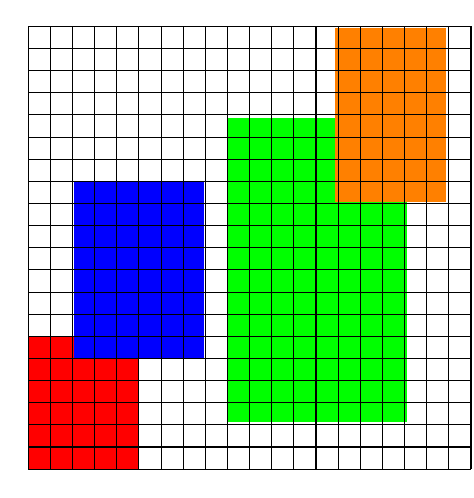
\begin{tikzpicture}(1,1)
  \draw [fill=red,red] (0,0) rectangle (1.39,1.68); 
  \draw [fill=blue,blue] (0.59,1.4) rectangle (2.23,3.65);
  \draw [fill=green,green] (2.55,0.6) rectangle (4.8,4.45);
  \draw [fill=orange,orange] (3.9,3.4) rectangle (5.3,5.6);
  \multiput(0, 0)(8, 0){21}{\line(0, 1){160}}
  \multiput(0, 0)(0, 8){21}{\line(1, 0){160}}
 \end{tikzpicture}
 \caption{5-colour image illustrating encoding redundancy}
 \label{COMP_ILLUS}
\end{figure}
\subsection{Predictive compression of KAT-7 data}
All compression techniques build on the central concept of reducing redundant data as pointed out previously. The exact definition of this redundancy is of course context 
dependent. In the case of the KAT-7 / MeerKAT array this redundancy may be defined in terms of the coherency of consecutive observations from each pair of dishes 
(or \textit{correlated} pairs). If the observations made are not particularly noisy it is reasonable to assume that the differences between consecutive values will be small.
Rather than storing each value it is possible to store the differences between observations (over a fixed time interval) instead. See figure~\ref{MeerKAT_PIPELINE}. 
The array observes a large spectrum of frequencies over a large number of correlated pairs, as indicated in the illustration. Each of these correlated frequency 
observations can be considered as steps of a time series. This report investigates how linear prediction can be employed to predict consecutive values for each of these time 
series. The goal is to minimise the difference between consecutive values, which can then be encoded using fewer bits than the original 32-bit sample size that is received 
by the processing and storage cluster. Such a scheme has the additional requirements of being \textit{lossless}, \textit{online} and fast.

\begin{figure}[h!]
 \centering
 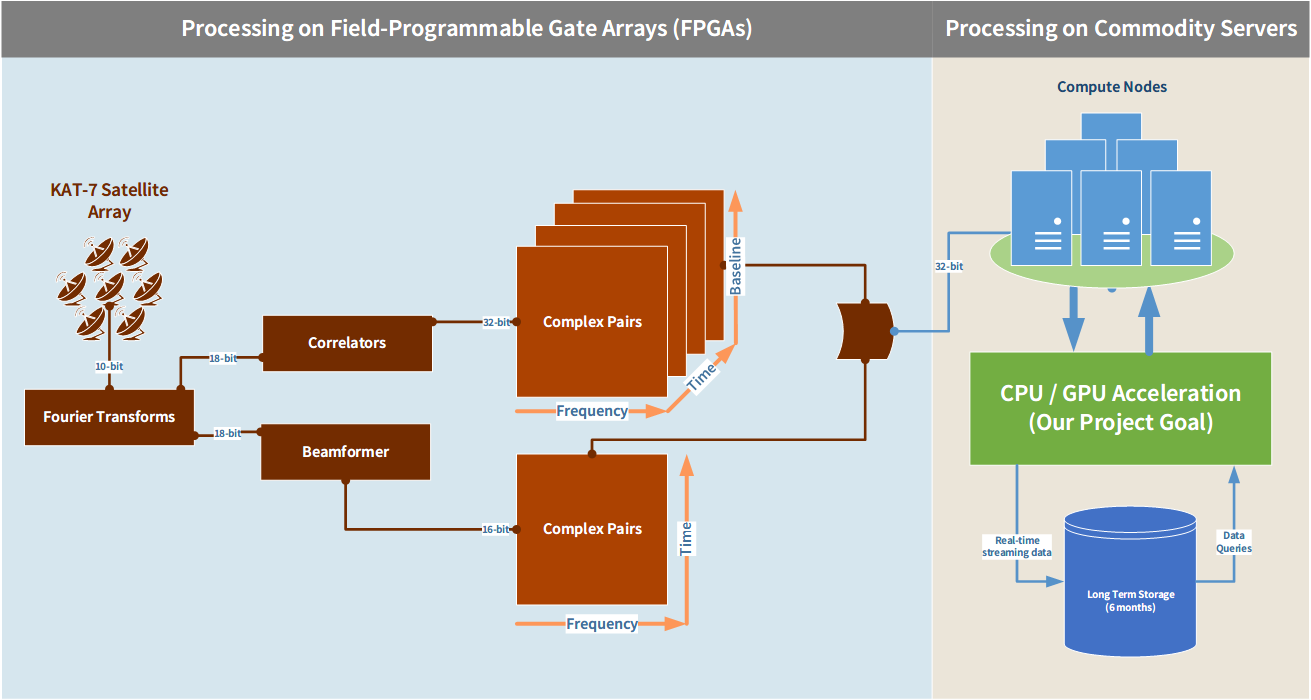
\includegraphics[width=0.8\textwidth]{Process.png}
 \caption{High-level overview of the MeerKAT pipeline}
 \label{MeerKAT_PIPELINE}
\end{figure}
\subsection{Compression algorithm properties and measurements}
In a lossless compression scheme the compression is completely invertible with \textit{no} loss of information after a decompression step is performed. Lossy
compression on the other hand discards unimportant data and gives much higher compression ratios than lossless methods. Lossy compression is useful in many
instances where subtle changes in data is not considered problematic. Some examples of this are the removal of high frequency data from images, sampling 
voice data at a lower rate than music or to employ a commonly used technique called \textit{quantization} where data is simply binned into consecutive ranges 
(or \textit{bins}).

An online compression scheme refers to a process of compressing data on-the-fly as it is being transmitted. The results are sent off to subsequent 
processes such transmission over a network or storage to disk. This is in contrast to to an offline scheme where data is compressed as a separate process which does not
form part of the primary work-flow of a system. An online process is normally required to be fast enough, as not to slow the overall data processing capabilities of 
a system.

Compression performance will be measured both in terms of effectiveness through a compression ratio described below \cite[p. 10]{salomon2004data} and throughput. A 
compression ratio closer to 0 indicates a smaller output file and values greater than 1 indicates that the algorithm inflated the data instead of shrinking it.
\begin{equation}
 \text{Compression ratio} := \frac{\text{size of the output stream}}{\text{size of the input stream}}
\end{equation}
\begin{equation}
 \text{Throughput} := \frac{\text{input processed (in GB)}}{\text{difference in time (in seconds)}}
\end{equation}
\subsection{Research questions}
Due to the limited scope of the project this report will only focus on evaluating algorithm performance and not algorithm integration into the KAT-7 / MeerKAT processing
pipeline. This research will include the construction of a parallel algorithm, as well as the investigation of the feasibility of porting this algorithm to the General 
Purpose Graphics Processing Unit (GPGPU)-accelerated nodes currently employed by the KAT-7 signal processing nodes as illustrated in figure~\ref{MeerKAT_PIPELINE}.

The algorithm will have to meet two primary criteria: high throughput and effective compression ratios. These are outlined below:
\begin{enumerate}
 \item Are predictive techniques fast enough? The algorithm should be able of achieving throughput rates of at least 40 GiB/s. These represent Infiniband network speeds 
 and represents a reasonable first milestone towards achieving compression at line rates.
 \item Are predictive techniques effective? The algorithm should reduce the size of transmissions by several percent and hopefully this reduction can take the form of 
       double digit figures. It has, however, been pointed out by the SKA office that the data may be too noisy to expect great reductions, while maintaining the throughput 
       rate mentioned above.
 \item Can throughput be traded for compression ratio using different predictors?
\end{enumerate}

Next a detailed breakdown of the most commonly used compression techniques is given. Thereafter a discussion will be given on a design of a predictive compression scheme, 
different implementation strategies, along with technical details, and a section with results and discussion.
\section{Background}
\subsection{Overview of data compression techniques}
There are considered to be 4 broad categories of compression techniques \cite{salomon2004data}. These are the basic methods, Lempel-Ziv methods, statistical methods 
and transforms.
\subsubsection{Basic methods}
The more intuitive methods include commonly employed methods such as Run-Length Encoding, which, simply put, encodes runs of characters using some reserved 
character and a number indicating the length of the run. In the context of compressing floating-point data such a scheme will focus on encoding runs of zeros and ones
at a bit level.

Another basic technique which is particularly relevant for application on numerical data is a predictive compression scheme. Such a compression scheme encodes the 
difference between each predicted succeeding value and the actual succeeding value as explained earlier. This can be quite successfully employed to compress data 
generated from time series \cite{engelson2000lossless}, but does rely on data coherence.
\subsubsection{Lempel-Ziv methods}
Lempel-Ziv is commonly referred to as “LZ” or dictionary methods, is a class of algorithms with many variants. It is one of the more popular \textit{adaptive} techniques 
in modern compression utilities. In their simplest form these methods normally use both a search- and lookahead buffer to encode recurrent phrases using fixed-size codes. An 
adaptive compression technique is useful in circumstances where the probability distribution of the underlying dataset is not known in advance or may change over time. 
One example of such an LZ method is used in the GNU compression utility Gzip. Gzip implements the DEFLATE algorithm which is a variant of the first LZ scheme, LZ-77 
\cite[ch. 3]{salomon2004data}.

LZ-77 encodes these recurrent phrases as length-distance pairs. If a sequence of characters are found to be the same as a sub-sequence of characters in the search buffer the 
distance to the start of that sub-sequence together with the length of the match is encoded. The size of the search buffer can be up to 32 kB in some implementations of the 
algorithm \cite[ch. 3]{salomon2004data}.
\subsubsection{Statistical methods}
This class of algorithms normally uses variable-length codes to achieve an optimal (or near optimal) encoding of dataset. In information theory this optimal encoding is 
described as an \textit{entropy} encoding. Entropy is the measurement of the information contained in a single base-n symbol (as transmitted per unit time by some source).

Redundancy is defined as the difference in entropy between the optimal encoding and the current encoding of a data set and is expressed in the following equation  
($n$ is the size of a symbol set and $P_{i}$ is the probability that a symbol $c_{i}$ is transmitted from a source)\cite[p. 46 - 47]{salomon2004data}:
\begin{equation}
 R := \log_2n + \sum_1^nP_i\log_2P_i
\end{equation}
As the name may suggest these techniques use the probability of occurrence of a value to assign shorter codes to frequently occurring values in order to eliminate redundancy. This 
class include two widely employed techniques known as Huffman and Arithmetic coding respectively. Huffman coding assigns shorter \textit{integral-length} codes, while arithmetic 
coding assigns \textit{real-length} subintervals of [0,1) to frequently occurring symbols \cite{Witten:1987:ACD:214762.214771}\cite[ch. 2]{salomon2004data}.

Huffman coding counts the number of occurrences of a particular symbol, sorts this list in ascending order and merges the rarest pairs of symbols into a single \textit{binary} 
(a tree in which each node can have up to 2 children) sub-tree and re-inserts the merged sub-tree into the list (still preserving the previously established order). The number of occurrences 
of each subtree will be the sum of occurrences of all the leaf nodes. Upon termination of this process only a single binary tree is left in the list. Each left-traversal adds a 0 to the encoding 
of a symbol, while each right-traversal adds a 1. When a leaf-node is reached the constructed encoding is an \textit{unambiguous} code for the symbol. Refer to figure~\ref{HUFFMAN} for an example.
In this case the symbol \textit{H} will be represented as 11 while some of the least frequent symbols such as \textit{B} will be represented by a longer code (0001 in this case).
\begin{figure}[h!]
 \centering
 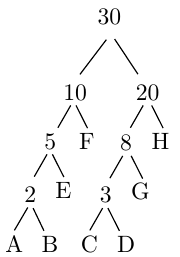
\includegraphics[width=0.15\textwidth]{huffmanTree.png}
 \caption{Sample of a completed Huffman-coding binary tree \cite[p. 70]{salomon2004data}}
 \label{HUFFMAN}
\end{figure}

Instead of assigning variable, \textit{integral}, length codes per symbol as is done by Huffman coding, Arithmetic coding encodes an entire message as a sub-interval of [0,1). As with
Huffman a probability distribution has to be determined (or be specified) before the algorithm can be executed. The initial interval [0,1) is reduced by each consecutive 
symbol. The length of the sub-interval is proportional to the probability of occurrence of the symbol being read. The final symbol gets assigned any value inside the remaining 
sub-interval. As the interval decreases the number of bits required to encode each consecutive interval increases. However, the average number of bits needed to store 
each symbol is closer to the that of the entropy encoding of the dataset, since this average number can be \textit{real} value, unlike that of the per-symbol encoding of Huffman \cite[ch. 2]{salomon2004data}.

Both approaches lead to variable-size codes. Both techniques have adaptive versions which are useful in situations where the probability distributions change or have to be estimated. 
This approach is also applicable to the situation where the symbol table has to be computed on the fly, because it is impossible to perform multiple passes over data. This can, for example
be the scenario when processing streaming data and all compression has to be completed on the fly. Arithmetic coding achieves higher compression ratios in both adaptive and non-adaptive cases 
when compared to Huffman coding. It should be pointed out that the decompression step of Arithmetic coding is slow and unsuitable for cases where fast access is 
required \cite{ray1995database,williams1999compressing}\cite[ch. 2]{salomon2004data}.

\subsubsection{Transforms}
As the name suggest it can be useful to transform a dataset from one form to another in order to exploit its features for the purposes of compression. Such transformations 
includes, for example, wavelet transforms. As the name suggests a wavelet is a small wave-like function that is only non-zero over a very small domain and is useful
to separate the low frequency components from the high frequency components of, for example, an image. JPEG2000 and DjVu are popular formats that use 
wavelet transforms. The dataset is generally sampled at increasing frequencies to produce a series of representations that gradually increases in resolution. When added together 
these representations will reconstruct the original dataset. A sample of the discrete cosine transform of an image (as employed by JPEG2000) is shown in figure~\ref{TRANSFORM_SAMPLE}. 
Only the transformation coefficients have to be stored in order to reconstruct each value in this series. The coefficients within this transformation can then be further compressed 
using other techniques, for example, Huffman coding and Run-Length Encoding (as is done in JPEG2000). If lossy compression (loss of accuracy which cannot be recovered after 
decompression) is tolerable, quantization can be used to discard unimportant values (for example the high frequency features of an image) \cite{952804}\cite[ch. 5]{salomon2004data}.
\begin{figure}[h!]
 \centering
 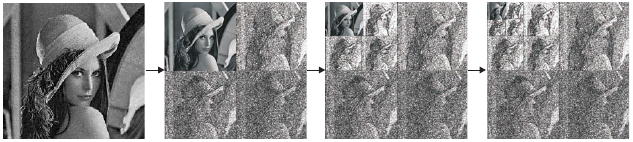
\includegraphics[width=1.0\textwidth]{DCTSample.png}
 \caption{Sample output from a Discrete Cosine Transform employed by JPEG2000 \cite{952804}}
 \label{TRANSFORM_SAMPLE}
\end{figure}

Transforms are furthermore particularly useful where multiple levels of detail are desired. An example of this may include the transfer of scientific data over a network 
for real-time analysis and observation. Low resolution samples can be consistently transferred, while higher resolution samples can be transferred upon request \cite{Tao:1994:PTS:951087.951108}.
\subsection{Overview of predictive compression}
Previous research \cite{1607248,4589203,engelson2000lossless,lindstrom2006fast,O'Neil:2011:FDC:1964179.1964189,4976448,CGF:CGF681} in this area has yielded good results both in terms of compression ratio and speed. 
The common line of thought is to predict successive values with reasonable precision. Depending on the accuracy of the prediction, the difference between the predicted and actual value will be much smaller than the actual value itself. 
This difference can then be encoded using fewer bytes/bits of data (depending if compression occurs at a byte or bit level) by compressing the leading zeros after either an XOR or integer subtraction 
operation. Machine instructions to count the leading zeros can be found on AMD and newer Intel Processors. The leading zero count is then encoded as a prefix stream while the remaining bits/bytes 
are encoded as a residual stream.

Previous research suggests several different constructions of predictors. The use of a \textit{Lorenzo} predictor \cite{lindstrom2006fast,CGF:CGF681} generalizes the well known parallelogram predictor. 
The Lorenzo predictor extends the parallelogram to arbitrary dimensions. More detail on the parallelogram predictor will be given
in the implementation section, but it is useful to note that this approach is particularly useful for compressing large meshes. Other approaches include the use of prediction history 
(via a simple lookup table construction) as suggested by Burtscher et al. \cite{1607248,4589203,4976448}. Burtscher et al. reports a throughput of up to 670 MB/s on a CPU implementation of their FPC 
compressor. An even simpler scheme by O'Neil et al. \cite{O'Neil:2011:FDC:1964179.1964189} reportedly achieved throughputs of up to 75GB/s for compression and up to 90GB/s 
decompression, implemented in CUDA. In this scheme only the difference between successive values are encoded (this will clearly only work if pairs of data points 
vary very little from one time step to the next). It is duly noted that the speeds achieved  are on the post-processing of results, already stored in graphics memory. 
The implementations by \cite{O'Neil:2011:FDC:1964179.1964189,1607248,4589203,4976448,engelson2000lossless} target 64-bit IEEE 754 
\textit{double} precision floating-point data.

The IEEE 754 standard of 2008 defines 3 interchange formats (32-bit, 64-bit and 128-bit). See figures~\ref{IEEE_FLOAT}~\&~\ref{IEEE_FLOAT_TAB}. Each of these have a common 
construction with the following subfields:
\begin{itemize}
 \item A 1-bit sign
 \item A w-bit length biased exponent
 \item A (d-1)-bit significand, where the leading bit of the significand is implicitly encoded in the exponent.
\end{itemize}
\begin{figure}[h!]
 \centering
 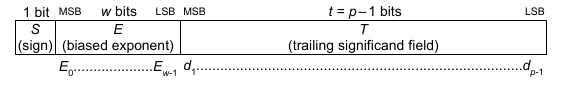
\includegraphics[width=0.6\textwidth]{IEEEinterchangeFormat.png}
 \caption{IEEE Interchange floating-point format \cite{4610935}}
 \label{IEEE_FLOAT}
\end{figure}
\begin{figure}[h!]
\centering
\begin{tabular}{|c|c|c|}
 \hline
 Precision & Exponent width & Significant precision \\
 \hline
 32-bit & 8 bits & 23 bits \\
 \hline
 64-bit & 11 bits & 52 bits \\
 \hline
\end{tabular}
\caption{Specifications for the 32-bit and 64-bit interchange formats}
 \label{IEEE_FLOAT_TAB}
\end{figure}
The primary scheme proposed in this paper takes its inspiration from the work of O'Neil et al. \cite{O'Neil:2011:FDC:1964179.1964189}, but will operate on 32-bit 
IEEE 754 \textit{single} precision floating-point values, as pointed out in the introduction. The uncompressed data itself is also structured slightly 
differently to the model used by O'Neil et al. \cite{O'Neil:2011:FDC:1964179.1964189}. Instead of compressing each consecutive value the proposed compressor will operate 
over consecutive time slices (refer to figure~\ref{MeerKAT_PIPELINE}).

As pointed out in previous research \cite{engelson2000lossless,lindstrom2006fast} using floating-point operations in the prediction step can cause an irreversible loss of information due to floating-point
rounding errors. A simple alternative approach is proposed by Engelson et al. \cite{engelson2000lossless}: floating-point memory is simply treated as integer memory and all operations performed on that memory are integer operations. This
approach ensures the predictive scheme achieves lossless compression. In light of this only schemes that conform to this approach will be considered. Engelson et al. \cite{engelson2000lossless} gives an example of how floating-point numbers
can be treated with integer operations. Figure~\ref{INT_REP} shows that if two floating-point numbers are relatively close to each other in terms of magnitude it is possible to discard some repeated bytes of information after performing 
an XOR operation to extract the remaining, seemingly random, residual bits. Therefore if an accurate prediction can be made for consecutive numbers a reasonable
saving in terms of compression ratio can be made.
\begin{figure}[h!]
\centering
\begin{tabular}{|c|c|c|c|}
 \hline
  & & byte & 1\hspace{8 pt}2\hspace{8 pt}3\hspace{8 pt}4\hspace{8 pt}5\hspace{8 pt}6\hspace{8 pt}7\hspace{8 pt}8\\
 \hline
 $a_{1}$ & 2.3667\textbf{1}76745585676 & $\Rightarrow$ & 40 02 ef \textbf{09 ad 18 c0 f6} \\
 \hline
 $a_{2}$ & 2.3667\textbf{2}76745585676 & $\Rightarrow$ & 40 02 ef \textbf{0e eb 46 23 2f} \\
 \hline
 $a_{3}$ & 2.3667\textbf{3}76745585676 & $\Rightarrow$ & 40 02 ef \textbf{14 29 73 85 6a} \\
 \hline
\end{tabular}
\caption{Treating 64-bit IEEE 754 double precision floating-points as integer memory \cite{engelson2000lossless}}
 \label{INT_REP}
\end{figure}
\section{Design and Methodology}
\subsection{Overview}
In light of the research questions and the limited scope of this report focus will be placed on the usefulness of a predictive data compression 
step in the context of the MeerKAT project. This will be limited to an investigation on whether the algorithm can operate at the desired line rate of
40 GiB/s and whether it provides reasonable compression ratios. This initial investigation precludes the implementation of the algorithm as part of 
the networking stack employed in the KAT-7 pipeline. Reasonable compression in this context means achieving compression ratios, comparable to industry standard 
tools like GZIP and BZIP2. The possibility of using alternative predictive schemes to trade some throughput for a better compression ratio will also be investigated.
Such alternative schemes will include the following (notes on their efficient implementation will be provided in the implementation section):
\begin{enumerate}
 \item A Lagrange polynomial extrapolation.
 \item A parallelogram predictor.
 \item Moving mean \& median predictors.
\end{enumerate}
The key success criteria for this investigation are the following:
\begin{enumerate}
 \item Throughput in excess of 40 GiB/s is achieved by both the compressor and decompressor.
 \item Effective compression ratios, comparable to those achieved by GZIP and BZIP2 are achieved.
\end{enumerate}
\subsection{Packing algorithm}
The compacting algorithm being proposed is based on the approach taken by O'Neil et al. \cite{O'Neil:2011:FDC:1964179.1964189}. The algorithm is almost \textit{symmetrical} in its compression and 
decompression stages. In this context symmetry means the algorithm is executed in the opposite direction when performing decompression. The primary difference is that the leading 
zero count does not have to be computed for each element being decompressed. Refer to figure~\ref{PACKING_ALGORITHM} for more details.
\begin{figure}[h!]
 \centering
 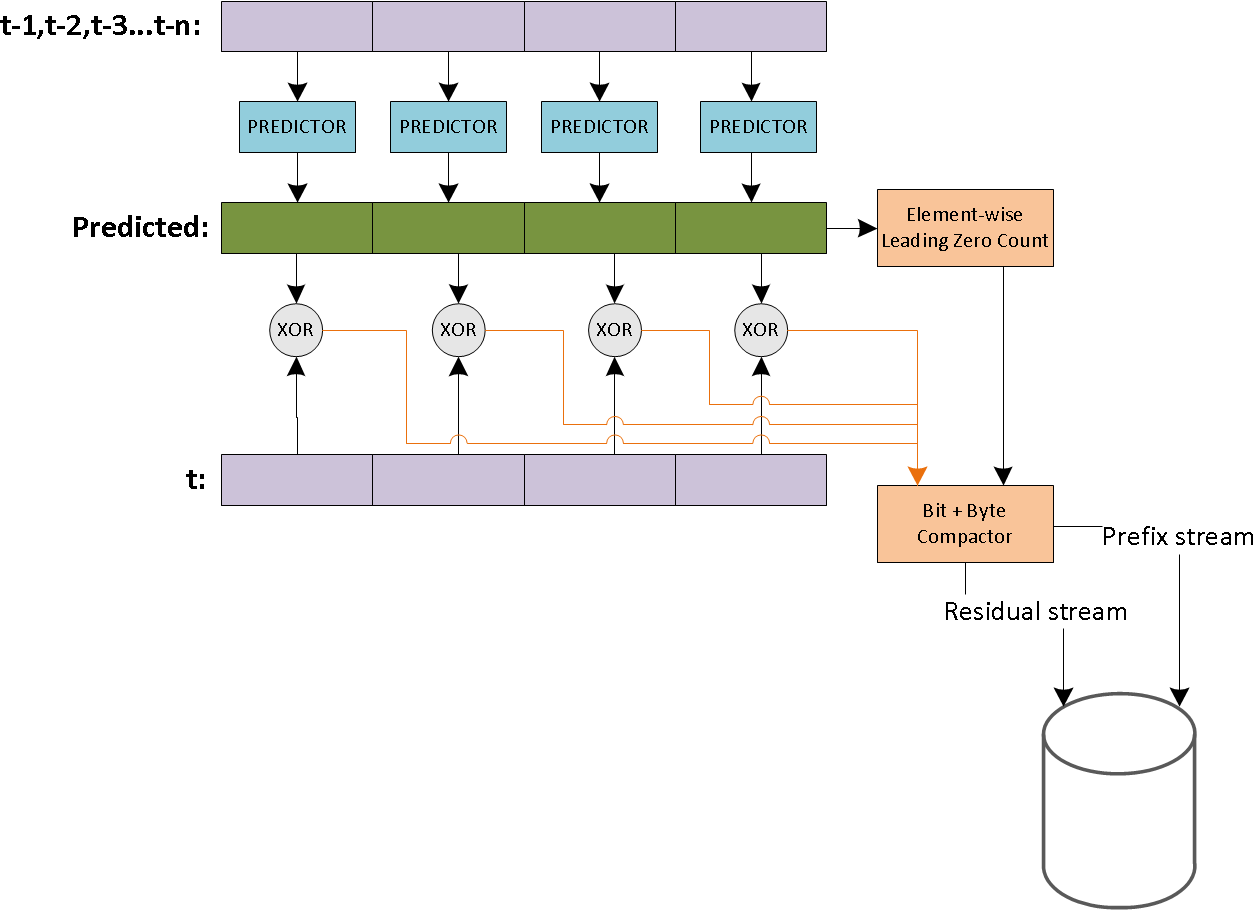
\includegraphics[width=0.7\textwidth]{Thesis_Alg.png}
 \caption{Prediction and compaction process}
 \label{PACKING_ALGORITHM}
\end{figure}
The construction of the algorithm being specified in figure~\ref{PACKING_ALGORITHM} is used because it allows for easy swapping between different predictors. The predictor in this case 
can be any n-element predictor. As mentioned earlier the predicted value is XORed with the actual value to get a residual which can be compacted at either bit or byte level. This 
compaction simply removes the leading zeros from each residual and stores each residual as a fixed-length prefix count. The number of bits needed to store $n$ leading 
zeros can be calculated as $\lfloor\log_2n\rfloor+1$ bits where $n\in\mathbb{N}_{>0}$. It remains to find the residual compaction scheme that gives the best results: packing at 
bit or byte level. Although a bit-packing scheme can pack an arbitrary number of zeros it requires longer prefixes to store the leading zero counts. The opposite is true 
for byte-packing schemes. Since the prefixes are always short a bit-packing scheme is used to store these fixed-length codes. Basic pseudo code is given in the implementation section.

Suppose the following two converted float values have to be compacted (the left-most byte is the most significant byte):
\begin{center}
  \begin{verbatim}
    #1: 00000000 01100010 01101000 11001001
    #2: 00000000 00000000 11110001 11110010
  \end{verbatim}
\end{center}
In this scenario the compaction of the residuals is done at byte level and the prefixes are done at bit level (assume 3 bits are needed to store up to 4 bytes of leading zeros):
\begin{center}
  \begin{verbatim}
    RESIDUALS:
    01100010 01101000 11001001 11110001 
    11110010
    PREFIXES (VALUES ARE PADDED UP TO ENSURE ONLY COMPLETE BYTES ARE STORED):
    00101000
  \end{verbatim}
\end{center} 
\subsection{Parallelizing compression and decompression steps}
There are three ways this can be achieved: 
\begin{enumerate}
 \item Even though the residuals are of variable length it is possible to pack them in parallel. However, there is an additional overhead to \textit{both} the packing and 
 unpacking process, since this approach requires a prefix sum to be computed for the array of element-wise leading zero counts as O'Neil et al. \cite{O'Neil:2011:FDC:1964179.1964189} 
 points out.
 
 A prefix sum (or \textit{scan}) can be defined on any binary associative operator, $\oplus$ over an ordered set with $I$ as its identity. If $A=[a_{0},a_{1},\dots,a_{n-1}]$ 
 is an ordered set then the prefix sum scan is defined as $scan(A):=[I,a_{0},(a_{0} \oplus a_{1}),\dots,(a_{0} \oplus a_{1} \oplus ... \oplus a_{n-2})]$. 
 
 In the context of the packing scheme proposed here, the prefix scan is defined over the normal integer addition operator. An example of this will be $scan[2,1,3,4] = [0,2,3,6]$ 
 under normal integer addition. The leading zero counts are saved to an array, \textit{A}, after which the scan operation is computed on the array. The accumulated values are 
 stored in place and hence the algorithm has a \textit{constant} memory overhead (uses no extra memory). Each index \textit{A}[\textit{i}] will therefore store the starting 
 position (in bits) of the residual of the $i^{th}$ element \cite{blelloch1990prefix}. 

 This scan operation can be computed in parallel. Blelloch suggests such an approach \cite{blelloch1990prefix}. The algorithm will be discussed in greater detail in the 
 implementation section. Additionally a work-efficient CUDA version of the algorithm is discussed in GPU Gems 3 \cite{harris2007parallel}. In this version the algorithm is 
 optimized to avoid \textit{bank conflicts} (see the section on GPU architecture) and has been shown to be up to 6 times faster than a sequential CPU implementation for large 
 arrays.
 
 After the indexes have been accumulated using the prefix sum algorithm it is easy to see how different threads can pack residuals at the correct positions. Both a bit and byte
 packing scheme will, however, require \textit{atomic} operations to ensure against the \textit{race condition} that arises when multiple threads write to the same memory 
 location simultaneously. This memory-level-synchronization mechanism adds additional overhead in terms of wasted machine clock cycles.
 \item Incoming data can also be separated into blocks, after which multiple of these blocks can be done in parallel (where each block is compressed/decompressed in serial). This overcomes the issue of 
 additional overheads arising due to computing prefix sums and using atomics. This approach may have a detrimental effect on the compression ratio since the length of the residual array of each block 
 has to be stored.
 \item A more fine-grained parallelization is possible using vectorized instructions. The various Intel SSE, Steaming SIMD (Single Instruction Multiple Data) instruction set extensions (up to version 4.2) provide
 the opportunity to perform 4 instructions (adds, multiplies, logarithms, rounding, etc.) simultaneously per core. However, the SSE instruction sets do not have any element-wise bit-shift operations. A combination 
 of the Intel SSE and AMD XOP instruction sets, will however, provide enough support to write the most of the algorithm using vector intrinsics. The XOP instruction set extends the SSE instruction set by adding these 
 operations as one of its primary features. Adding these instructions will, however, make the implementation dependent on the architecture of the underlying machine it is executed on (and therefore less portable). 
 If this approach is successful the vectorized code should be extended to use the latest Intel AVX 2 instruction set in which Intel introduces element-wise shift operations and offset-loading operations in future work. 
 The AVX family of instructions can compute up to 8 SIMD operations in parallel per core. All these vectorized instruction sets make use of a very limited number of 128- and 256-bit registers (SSE and AVX respectively).
 It remains to be investigated whether it is worthwhile to implement the proposed packing algorithm using SSE and XOP instructions.
\end{enumerate}
\subsection{Porting the implementation to CUDA}
General Purpose programming using Graphics Processing Units (GPGPU) brings a host of associated challenges. These challenges arise primarily due to the widely differing architecture of GPUs if compared
with the classical architectures of Central Processing Units (CPUs). Refer to figure~\ref{FERMI_ARCH} for a detailed overview of the microchip die structure of a Nvidia Fermi generation GPU. 
However, each generation of GPUs have widely differing architectures, each making many architecture specific optimizations. Each generation, for instance, will have both a 
different ratio and configuration of arithmetic cores to floating-point and special operations cores, per group of processing \textit{CUDA cores}. These cores are also known as 
\textit{SMs} (or \textit{SMXs} on the latest \textit{Kepler} generation). Additionally each generation has widely differing memory controller layouts. These may determine 
how many \textit{warps} of threads can be executed, when the warps are swapped in/out, along with many others. Each SM is split into atomic groups of threads which are executed
in parallel (normally this is specified as 32 threads per warp). Even if only a subset of these threads have work the entire warp will be executed on the same machine clock cycle.

A basic CUDA implementation will be provided to see if doing compression as a post-processing step on signal data already loaded to GPU (as part of the current pipeline) is a 
feasible alternative to a regular multi-threaded CPU implementation. Adaquite use of shared memory (as figure~\ref{FERMI_ARCH} shows GPUs have very large L1 and L2 caches available per SM) 
will be made and the implementation will take adequate precaution to \textit{coalesce} memory accesses and to avoid \textit{bank conflicts} when possible. 

Coalesced memory accesses are made if a continuous chunk of memory is accessed by a half-warp of threads at the same time. Normally these accesses have to be made in a uniform pattern. 
Individual memory calls to global graphics memory is a very costly operation (and therefore random accesses have to be avoided). Coalesced accesses are made simultaneously by the 
memory controller. Such accesses retrieve / write memory in larger chunks, which counters the latency associated with such an access. 

In GPU architectures (at the very least with Nvidia cards) \emph{shared} memory is divided up into banks. When multiple threads (specifically a half-warp of threads) try to 
access the same bank of memory, the memory accesses will be made sequentially. The general approach to avoid such a situation is to add padding between blocks of shared memory.

More details will be provided in the implementation section, but it is clear that a combination of the approaches (1 \& 2) taken with the CPU version will be required to make 
adequate use of the GPU architecture. This proposed implementation will consider assigning a block of data to each SM, which will in turn process that block in parallel without 
regard to operations performed on other SMs. This ensures that no unnecessary overheads due to costly card-wide synchronization steps are introduced. Instead all atomic 
operations and synchronization steps will be performed per-SM only.
\begin{figure}[h!]
 \centering
 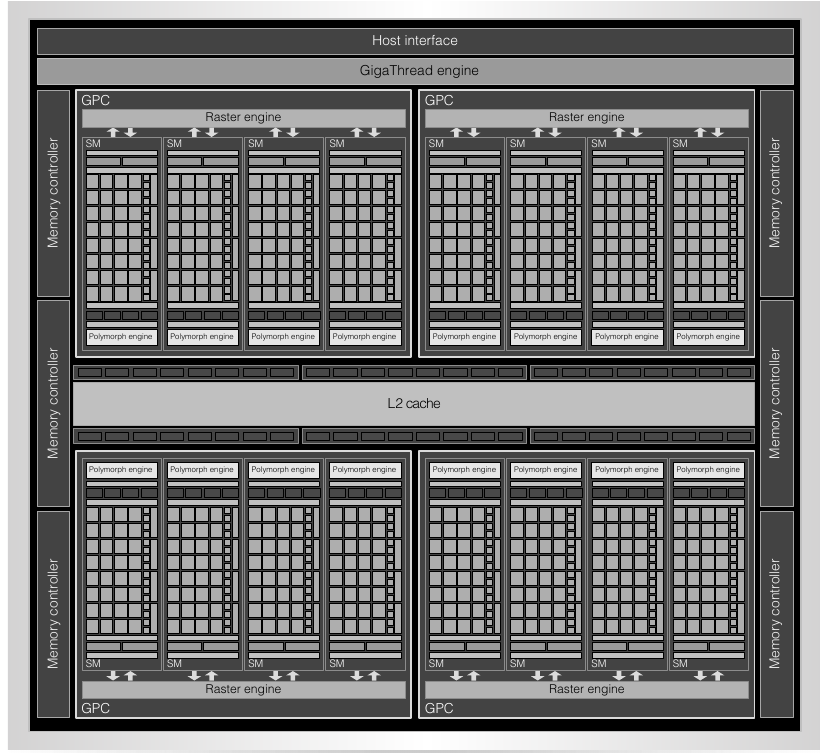
\includegraphics[width=0.8\textwidth]{fermi_arch.png}
 \caption{Architecture of the Fermi family of Nvidia GPUs \cite{wittenbrink2011fermi}}
 \label{FERMI_ARCH}
\end{figure}
\subsection{Test data}
The correlated data is provided in the form of HDF5 files. Each of these files stores a three dimensional array of complex pairs. The first dimension is time. The second 
is signal frequency (as mentioned in the background section the telescope array will monitor a wide range of frequencies). The third dimension is a combination of two 
properties. Each number represents a correlation between two antennae. The antennae additionally have two modes of polarization (a horizontal and vertical polarization). 
The size of the last dimension is specified as two times the number of permutations of $n + 1$: $2\times((n+1)\mathbf{P}2)$ elements where $n$ is the number of
antennae in the array. The headers of the HDF5 files contain meta-information on the state of the telescope and what it is currently observing (this will determine the 
characteristics of the data itself as well as the range of frequencies being monitored). 

It should be noted that the headers cannot be compressed with the algorithm being proposed. An LZ variant / entropy encoder may be better tailored for this task. 
The headers vary between 13-14\% of the total h5 file size. However, the data is only written to these formats after it is received by the processing cluster (see 
figure~\ref{MeerKAT_PIPELINE}). Therefore if the algorithm being proposed is integrated into the front end of the pipeline as seen in figure~\ref{MeerKAT_PIPELINE} (as part of 
future work) it may still provide a significant saving in network I/O. 
\subsection{Structure and scope of the benchmarks}
Some of these HDF5 files measure more than 30GB in size, each containing many timestamps, some spread over 4000 frequencies. It is reasonable to assume that once the number of correlations grow, emphasis will be placed on processing each 
time step (or portion thereof) as soon as it is received over the network. In future research the compressor may be integrated into the 7-layer OSI networking stack currently employed by the KAT-7 prototype. Due to the limited
scope of this project focus will be on analyzing the performance of the algorithms themselves and not to measure any disk I/O (except when comparing to other compression utilities for the sake of fairness).

This report will focus on the following analysis:
\begin{enumerate}
 \item A comparison between the a CPU implementation of the parallel (prefix sum-based algorithm) and the blocked approach (as specified previously) will be made.
 \item A detailed breakdown of how the algorithm performs on different numbers of cores (of whichever method is determined most fit in step 1) will be provided.
 \item The effectiveness of a parallelogram predictor, a Lagrange extrapolation predictor \cite{engelson2000lossless} and a moving mean and median scheme will be determined. 
       Each of these methods will be described in greater detail in the implementation chapter.
 \item The feasibility of implementation using the Intel SSE and AMD XOP vectorized instruction sets will be investigated.
 \item Benchmarks of the algorithm against the standard programs used for comparison: GZIP, BZIP2, ZIP and RAR. In this case the disk I/O will be included for the sake of fairness.
 \item The feasibility of a CUDA implementation, as outlined earlier will be determined.
 \item Finally results from concurrent research being conducted into entropy encoding and run-length encoding will be compared to those achieved in this investigation. This comparison will include a 
       breakdown of performance in terms of both throughput and compression ratios.
\end{enumerate}
\subsection{Benchmarking platform}
The benchmarking platform is designed with two primary software engineering goals in mind:
\begin{itemize}
 \item It should be as \textit{decoupled} as possible, making use of predefined interfaces. This will assist in providing several implementations of the CPU version (for example SSE, different linear predictors and different parallelization
 approaches) and simply swapping one implementation for another. Interactions between components must be kept to a minimum.
 \item The components must be \textit{cohesive}. They should contain only relevant operations and should be considered as atomic units.
\end{itemize}
The architecture described in figure~\ref{TOOL_ARCH} is used for the benchmarking platform. All the external dependencies depicted in the component model is freely available
and are actively maintained. There is no considerable technical risk in using these libraries. More detailed implementation details will be provided in the next section. The 
benchmark process is relatively simple and its flow is depicted in figure~\ref{TOOL_FLOW}.
\begin{figure}[h!]
 \centering
 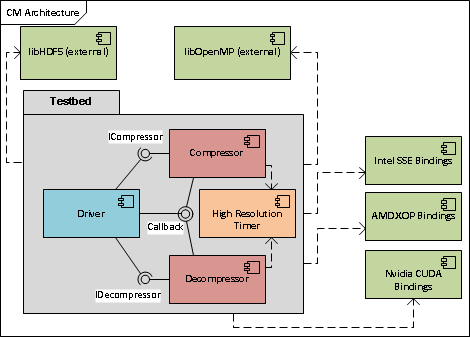
\includegraphics[width=0.6\textwidth]{Thesis_Arc.png}
 \caption{Architecture of the loosely coupled benchmarking platform, including external library dependencies}
 \label{TOOL_ARCH}
\end{figure}
\begin{figure}[h!]
 \centering
 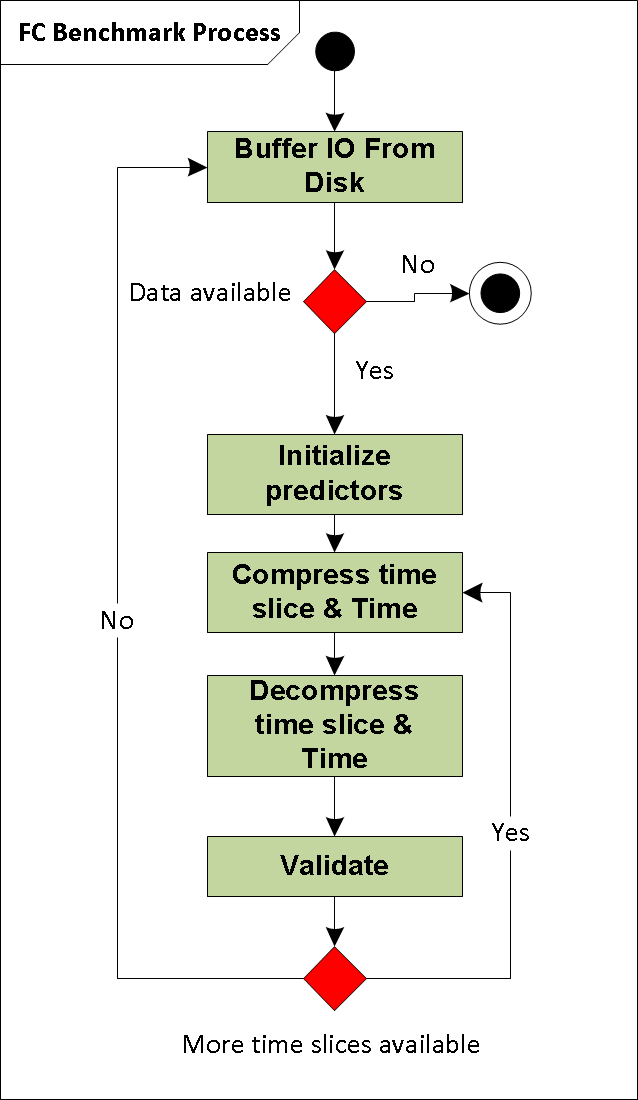
\includegraphics[width=0.25\textwidth]{Thesis_Flow.png}
 \caption{Behavioral model of the benchmarking platform}
 \label{TOOL_FLOW}
\end{figure}
\section{Implementation}
 \subsection{Basic algorithm}
  In order to give a more detailed description to the algorithm illustrated in figure~\ref{PACKING_ALGORITHM} in the previous section, the pseudo code for the compaction
  process is given below:
\begin{verbatim}
SUBROUTINE Compact(FLOAT[] data, UNSIGNED INT32 numElements, 
		    out UNSIGNED INT32[] residuals, 
		    out UNSIGNED INT32[] prefixes)
	 //ASSUMPTION: 3 BITS NEEDED TO STORE UP TO 4 BYTES OF LEADING ZEROS
	 //ASSUMPTION: COMPACTION IS DONE INTO 32 BIT INTEGER ARRAY
BEGIN
	 UNSIGNED INT32 bitPosInResidualArray = 0
	 FOR index = 0 TO numElements - 1 DO
		  /*
		  This prediction step requires up to "n" arrays of the 
		  same size of "data".
		  */
		  UNSIGNED INT32 predictedValue = linearPredict(index) 
		  UNSIGNED INT8 leadingZeroCount = clz(data[index])
		  UNSIGNED INT32 difference = predictedValue XOR data[index]
		  //save the prefix:
		  prefixes[index*3 INT_DIV 32] = SHIFT (leadingZeroCount INT_DIV 32) to \\
		    the index*3 MODULO 32 th bit
		  IF there are remaining bits that couldn't be fitted THEN
		    prefixes[index*3 INT_DIV 32 + 1] = SHIFT remaining bits that couldn't \\
		      be fitted in the previous operation to the first bit of the next byte
		  END IF
		  //save the residual:
		  residuals[bitPosInResidualArray INT_DIV 32] = SHIFT (difference to \\
		    the bitPosInResidualArray MODULO 32 th bit
		  IF there are remaining bits that couldn't be fitted THEN
		    residuals[bitPosInResidualArray INT_DIV 32 + 1] = SHIFT remaining bits \\
		      that couldn't be fitted in the previous operation to the first bit \\
		      of the next byte
		  END IF  
		  //increment position in the residual array
		  bitPosInResidualArray += leadingZeroCount INT_DIV 8
	 END FOR
END SUBROUTINE
\end{verbatim}
 \subsection{Alternative linear prediction schemes}
  The most basic prediction scheme simply encodes the difference between observations at time \textit{t} and $t+1$. This difference is given as $O[t]$ xor $O[t-1]$. This 
  scheme is sensitive to the structure of the underlying data. Such a scheme will only work if most consecutive values varies slowly over time. Using an n-element 
  predictor may help mitigate the effects of noise. However, as pointed out earlier: any operations over these n-elements have to be integer operations and not 
  floating point operations due to the rounding errors they may introduce (as pointed out in the background section). All floating-point memory are therefore cast to 
  integer-typed memory before values are retrieved.
  
  These predictions, however, still have to be fast and preferably have an average linear computational complexity, $\theta(n)$. The predictor will only 
  store the previous \textit{n} observations in a fixed-length queue. This implies that the memory overhead for the predictor is $nxm$ where m is the total 
  number of elements being processed at time $t$.
 \subsubsection{Lorenzo predictor}
 The n-dimensional Lorenzo predictor is a generalization of the two dimensional parallelogram predictor (see figure~\ref{LORENZO}). It can be used to predict scalar 
 functions that are polynomials of degree $n - 1$ and has been proven useful in scalar field compression \cite{CGF:CGF681}. In each of the 3 cases below only simple
 integer additions and subtractions are needed: the sum of the values in red are subtracted from the sum of the values in green. In the two dimensional case this 
 addition and subtraction is known as the \textit{parallelogram rule}. The predicted value is computed from previous observations as as $P = O[t-1] + O[t-2] - O[t-3]$.
  \begin{figure}[h!]
    \centering
    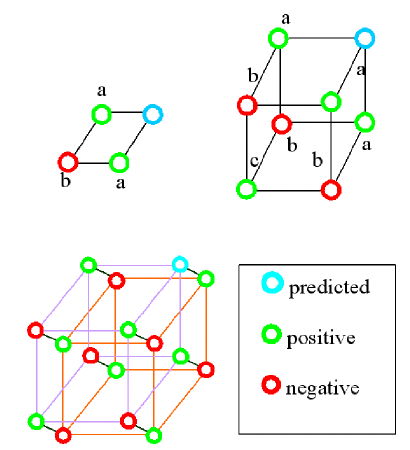
\includegraphics[width=0.3\textwidth]{lorenzo.png}
    \caption{Lorenzo predictor for 2D (upper left), 3D (upper right) and 4D (lower left) data \cite{CGF:CGF681}}
    \label{LORENZO}
  \end{figure} 
 \subsubsection{Moving average and moving mean}
  An integer-based moving mean is simple to implement and involves only a sumation and an integer division and therefore clearly has a linear computational complexity.
  However, the mean of a sample is sensitive to outliers, and therefore will not work well for noisy data. A simple solution will be to use a median based scheme
  where the predicted value is the center value of a \textit{sorted} list of observations. However, a naive implementation of such a median-based scheme will
  be slow due to the overheads of sorting. Wirth \cite{wirth76} suggests an algorithm to select the median using a basic \textit{pivoting} scheme in $\theta(n)$
  time. A pivot divides a dataset into two groups. The elements in the group to the right of the pivot is larger than the pivot and the elements in the group to
  the left of the pivot is smaller or equal to the pivot. The two groups do \emph{not} necessarily have to be ordered. The median is chosen through the following
  method that selects the \textit{k-th largest value} \cite{wirth76}:
  \begin{verbatim}
FUNCTION INT32 pivotMedian(INT32[] data, int n) {
    INT32 i, j, l, m, k = n/2-1 //k is the kth largest element in the array
    INT32 x, s

    l=0 //lower bound
    m=n-1 //upper bound
    WHILE l<m: //swap elements in group L and M until the two indexers cross
        x=data[k]
        i=l
        j=m
        REPEAT
	    //find 1 element in each sub-array that has to be swapped
	    //to the other sub-array:
            WHILE data[i]<x: i++
            WHILE x<data[j]: j--
            IF i<=j THEN
		    //swap:
                s=data[i]
                data[i]=data[j]
                data[j]=s
                i++
                j--
            END IF
        WHILE i<=j
        if(j<k) l=i
        if(k<i) m=j
    END WHILE
    RETURN data[k] //mid-point in the array
}
  \end{verbatim}
 \subsubsection{Lagrange prediction}
  {\color{red}TODO: Self.note.add also  include notes about the smoothness of data}
 \subsection{Algorithm parallelization}
  {\color{red}TODO}
 \subsection{SSE and XOP intrinsics} 
  {\color{red}TODO} 
 \subsection{GPGPU implementation in CUDA}
  {\color{red}TODO}
\section{Results}
\subsection{Constraints on benchmarking environment}
In order to eliminate the influence of the external testing environment the following special conditions are specified:
\begin{enumerate}
 \item Files in excess of 500 MB will be used for benchmarking. This will greatly reduce variability in timings.
 \item No other processes should be making intensive use of primary memory once benchmarking has commenced. The sheer quantity of data being processed makes benchmarking a memory-bound operation.
\end{enumerate}
\subsection{Parallelization approach}
\subsection{Performance of the block-based parallel scheme}
\subsection{Feasibility of including vector intrinsics}
\subsection{Benchmark against standard compression utilities}
\subsection{Feasibility of a CUDA implementation}
\subsection{Comparison to what was achieved in concurrent research}
\section{Discussion}
{\color{red}TODO}
\section{Conclusion}
{\color{red}TODO}
\section{Future avenues of research}
{\color{red}TODO}
\section{Glossary}
{\color{red}TODO}
\bibliographystyle{plain}
\bibliography{litRefs}
\end{document} to your LaTeX file where you want your
% title page.
%
%%%%%%%%%%%%%%%%%%%%%%%%%%%%%%%%%%%%%%%%%

%----------------------------------------------------------------------------------------
%	PACKAGES AND OTHER DOCUMENT CONFIGURATIONS
%----------------------------------------------------------------------------------------

\documentclass[12pt]{article}
\usepackage[utf8]{inputenc}
\usepackage{graphicx}
\usepackage{caption}
\usepackage{subcaption}
\usepackage{color}
\usepackage{amsmath}
\usepackage{amsfonts}
\usepackage[a4paper]{geometry}
\usepackage{fullpage}
\usepackage{parskip}
\usepackage{tikz}
\usepackage{hyperref}
\usepackage{mdframed}
\usepackage{pgfplots, pgfplotstable}
\usetikzlibrary{patterns}

\begin{document}

\begin{titlepage}

\newcommand{\HRule}{\rule{\linewidth}{0.5mm}} % Defines a new command for the horizontal lines, change thickness here

\center % Center everything on the page
 
%----------------------------------------------------------------------------------------
%	HEADING SECTIONS
%----------------------------------------------------------------------------------------

\textsc{\LARGE University of Cape Town}\\[1.5cm] % Name of your university/college
\textsc{\Large Department of Computer Science}\\[0.5cm] % Major heading such as course name
\textsc{\large CSC4000W - Honours in Computer Science}\\[0.5cm] % Minor heading such as course title

%----------------------------------------------------------------------------------------
%	TITLE SECTION
%----------------------------------------------------------------------------------------

\HRule \\[0.4cm]
{ \huge \bfseries Fast online predictive compression of radio astronomy data}\\[0.4cm] % Title of your document
\HRule \\[1.5cm]
 
%----------------------------------------------------------------------------------------
%	AUTHOR SECTION
%----------------------------------------------------------------------------------------

\begin{minipage}{0.4\textwidth}
\begin{flushleft} \large
\emph{Author:}\\
Benjamin \textsc{Hugo}\\ % Your name
\vspace{10pt}
\emph{Team members:}\\
Brandon \textsc{Talbot}\\ 
Heinrich \textsc{Strauss} 
\end{flushleft}
\end{minipage}
~
\begin{minipage}{0.4\textwidth}
\begin{flushright} \large
\emph{Supervisors:} \\
A/Prof. James \textsc{Gain}\\ % Supervisor's Name
Dr. Patrick \textsc{Marais}\\
\vspace{10pt}
\emph{External Advisor:} \\
Jason \textsc{Manley}
\end{flushright}
\end{minipage}\\[4cm]

% If you don't want a supervisor, uncomment the two lines below and remove the section above
%\Large \emph{Author:}\\
%John \textsc{Smith}\\[3cm] % Your name

%----------------------------------------------------------------------------------------
%	DATE SECTION
%----------------------------------------------------------------------------------------
\vspace{15pt}
\begin{center}
 A thesis presented to the Department of Computer Science, UCT, in partial fulfillment of the course CSC4000W, Honours in Computer Science.
\end{center}
\vspace{90pt}
{\large \today}\\[3cm] % Date, change the \today to a set date if you want to be precise

%----------------------------------------------------------------------------------------
%	LOGO SECTION
%----------------------------------------------------------------------------------------

%\includegraphics{Logo}\\[1cm] % Include a department/university logo - this will require the graphicx package
 
%----------------------------------------------------------------------------------------

\vfill % Fill the rest of the page with whitespace

\end{titlepage}

\begin{center} 
  {\LARGE Acknowledgements}
\end{center}
\vspace{50pt}

I would like to acknowledge A/Prof. James Gain and Dr. Patrick Marais of the Department of Computer Science at the University of Cape Town for their continuous, expert, input on the project.

Secondly I would like to thank Jason Manley, a Digital Signals Processing specialist at the MeerKAT offices in Pinelands, Cape Town for providing us with technical information
on the MeerKAT project. Jason has also kindly prepared a 100 GiB of sample of KAT-7 output data for testing purposes.

Thirdly I would like to note that all tests were performed on the ICTS High Performance (\textit{HEX}) cluster at the University of Cape Town. The cluster has 4 DELL C6145 nodes each boasting 4 16-core
AMD Opteron 6274 CPUs, clocked at 2200 MHz with 16 MiB L3 cache memory. There are two additional GPU nodes with 4 Tesla M2090 GPU cards each. Each GPU card has 6 GiB GDDR5 and 2048 CUDA cores. I want to 
especially thank Andrew Lewis from ICTS for his assistance and support during testing.

This research is made possible under grant of the National Research Foundation (hereafter \textit{NRF}) of the Republic of South Africa. All views expressed in this report are those of the author and not 
necessarily those of the NRF.
\pagebreak
\begin{abstract}
 {\color{red}TODO: add at end of writeup}
\end{abstract}
\pagebreak
\tableofcontents
\pagebreak
\section{Introduction}
\subsection{The KAT-7, MeerKAT and SKA}
South Africa and Australia are the two primary hosting countries for what is to become the largest radio telescope array in the world, known as the Square Kilometer Array (SKA). 
The SKA will give astronomers the opportunity to capture very high resolution images, over a wide field of view, covering a wide range of frequencies ranging 
from 70 MHz to 10 GHz. Upon completion in 2024 the array will consist of around 3000 dishes in the high frequency range and thousands of smaller antennae to 
cover the low frequency band. The South African branch of the SKA will be completed in 3 main phases. Phase 1 is a fully operational prototype 7-dish array 
called the KAT-7. The second phase, known as the MeerKAT, will consist of approximately 90 dishes. These are to be erected in the central Karoo region of South Africa. 
The final phase will add the remaining dishes and increase the baseline of the telescope to roughly 3000 km.

Due to the high signal sampling rate it is expected that each of these dishes will produce data rates of up to 420 GBit/s, while the lower frequency aperture arrays 
will produce up to 16 TBit/s. These rates, coupled with the scale of the SKA, will require a processing facility capable of handling as much as 1 Petabyte of 
data every 20 seconds, necessitating massive storage facilities. Innovative techniques are required to deal with the complex dual-requirement of high 
\textit{throughput rates} while effectively reducing the large storage requirements by means of \textit{data compression}. 
\subsection{Data compression \& decompression}
Data compression seek to encode data using a fewer number of bits than that of the original encoding. By removing such redundant data it is possible to effectively 
reduce the size of the dataset. A simple illustration of this can be found in figure~\ref{COMP_ILLUS}. It is clear that if this picture is stored naively as a 20x20
grid of 24-bit colours (8-bits for each of the red, green and blue channels) a lot of redundant data will be written to disk. A simple, yet effective, technique to 
reduce redundancy in this example is to store each horizontal line (or \textit{scanline}) of pixels as runs of colours, instead of individual colours. The first 
scanline can therefore be reduced to 9 white, 5 white, 5 orange, 1 white runs of pixels. This is known as \textit{Run-Length Encoding}. However, this is not the only 
form of redundancy: if each colour is represented as a 24-bit value, but only 5 colours are used from the $2^{24}$ colours available, a lot of storage space is wasted. 
In this case only  $\lfloor\log_{2}{5}\rfloor+1 = 4$ bits are needed to store all 5 colours uniquely. This variable-length encoding is often accomplished using an 
entropy encoding scheme which will be described to greater detail in the background section. Decompression can be thought of as the inverse operation to the compression 
process, which will reconstruct the original data from its encoded version.
\begin{figure}[ht!]
\begin{mdframed}
  \centering
 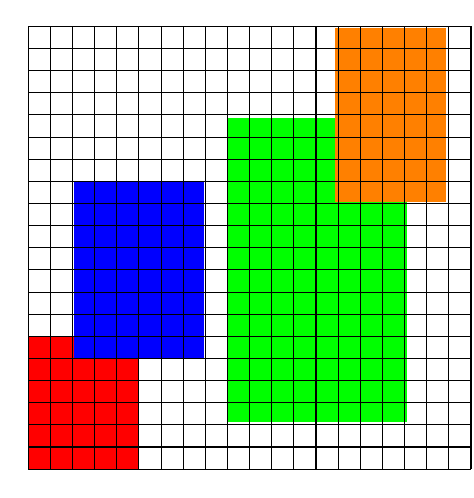
\begin{tikzpicture}(1,1)
  \draw [fill=red,red] (0,0) rectangle (1.39,1.68); 
  \draw [fill=blue,blue] (0.59,1.4) rectangle (2.23,3.65);
  \draw [fill=green,green] (2.55,0.6) rectangle (4.8,4.45);
  \draw [fill=orange,orange] (3.9,3.4) rectangle (5.3,5.6);
  \multiput(0, 0)(8, 0){21}{\line(0, 1){160}}
  \multiput(0, 0)(0, 8){21}{\line(1, 0){160}}
 \end{tikzpicture}
 \caption{5-colour image illustrating encoding redundancy}
 \label{COMP_ILLUS}
\end{mdframed}
\end{figure}
\subsection{Predictive compression of KAT-7 data}
All compression techniques build on the central concept of reducing redundant data as pointed out previously. The exact definition of this redundancy is of course context 
dependent. In the case of the KAT-7 / MeerKAT array this redundancy may be defined in terms of the coherency of consecutive observations from each pair of dishes 
(or \textit{correlated} pairs). If the observations made are not particularly noisy it is reasonable to assume that the differences between consecutive values will be small.
Rather than storing each value it is possible to store the differences between observations (each over a fixed time interval) instead. See figure~\ref{MeerKAT_PIPELINE}. 
The array observes a large spectrum of frequencies over a large number of correlated pairs, as indicated in the illustration. Each of these correlated frequency 
observations can be considered as steps of a time series. This report investigates how linear prediction can be employed to predict consecutive values for each of these time 
series. The goal is to minimise the difference between consecutive values, which can then be encoded using fewer bits than the original 32-bit sample size that is received 
by the processing and storage cluster. Such a scheme has the additional requirements of being \textit{lossless}, \textit{online} and fast.

\begin{figure}[h!]
\begin{mdframed}
 \centering
 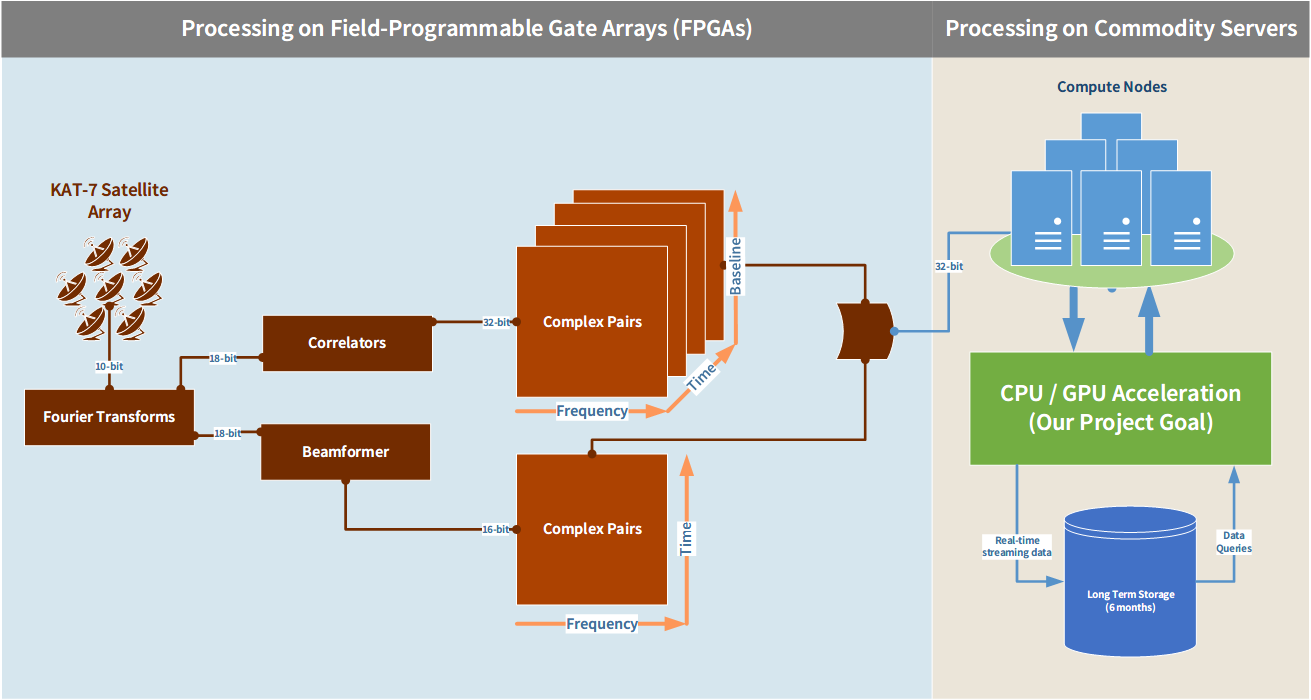
\includegraphics[width=0.8\textwidth]{Process.png}
 \caption{High-level overview of the MeerKAT pipeline}
 \label{MeerKAT_PIPELINE}
\end{mdframed}
\end{figure}
\subsection{Compression algorithm properties and measurements}
In a lossless compression scheme the compression is completely invertible with \textit{no} loss of information after a decompression step is performed. Lossy
compression on the other hand discards unimportant data and gives much higher compression ratios than lossless methods. Lossy compression is useful in many
instances where subtle changes in data is not considered problematic. Some examples of this are the removal of high frequency data from images, sampling 
voice data at a lower rate than music or to employ a commonly used technique called \textit{quantization} where data is simply binned into consecutive ranges 
(or \textit{bins}).

An online compression scheme refers to a process of compressing data on-the-fly as it is being transmitted. The results are sent off to subsequent 
processes such transmission over a network or storage to disk. This is in contrast to to an offline scheme where data is compressed as a separate process which does not
form part of the primary work-flow of a system. An online process is normally required to be fast enough, as not to slow the overall data processing capabilities of 
a system.

Compression performance will be measured both in terms of effectiveness through a compression ratio described below \cite[p. 10]{salomon2004data} and throughput. A 
compression ratio closer to 0 indicates a smaller output file and values greater than 1 indicates that the algorithm inflated the data instead of shrinking it.
\begin{equation}
 \text{Compression ratio} := \frac{\text{size of the output stream}}{\text{size of the input stream}}
\end{equation}
\begin{equation}
 \text{Throughput} := \frac{\text{input processed (in GiB)}}{\text{difference in time (in seconds)}}
\end{equation}
\subsection{Research questions}
Due to the limited scope of the project this report will only focus on evaluating algorithm performance and not algorithm integration into the KAT-7 / MeerKAT processing
pipeline. This research will include the construction of a parallel algorithm, as well as the investigation of the feasibility of porting this algorithm to the General 
Purpose Graphics Processing Unit (GPGPU)-accelerated nodes currently employed by the KAT-7 signal processing nodes as illustrated in figure~\ref{MeerKAT_PIPELINE}.

The algorithm will have to meet two primary criteria: high throughput and effective compression ratios. These are outlined below:
\begin{enumerate}
 \item Are predictive techniques fast enough? The algorithm should be able of achieving throughput rates of at least 40 GBit/s. These represent Infiniband network speeds 
 and is a reasonable first milestone towards achieving compression at line rates.
 \item Are predictive techniques effective? The algorithm should reduce the size of transmissions by several percent and hopefully this reduction can take the form of 
       double digit figures. It has, however, been pointed out by the SKA office that the data may be too noisy to expect great reductions, while maintaining the throughput 
       rate mentioned above.
 \item Can throughput be traded for compression ratio using different predictors?
\end{enumerate}

Next a detailed breakdown of the most commonly used compression techniques is given. Thereafter a discussion will be given on a design of a predictive compression scheme, 
different implementation strategies, along with technical details, and a section with results and discussion.
\section{Background}
\subsection{Overview of data compression techniques}
There are considered to be 4 broad categories of compression techniques \cite{salomon2004data}. These are the basic methods, Lempel-Ziv methods, statistical methods 
and transforms.
\subsubsection{Basic methods}
The more intuitive methods include commonly employed methods such as Run-Length Encoding, which, simply put, encodes runs of characters using some reserved 
character and a number indicating the length of the run. In the context of compressing floating-point data such a scheme will focus on encoding runs of zeros and ones
at a bit level.

Another basic technique which is particularly relevant for application on numerical data is a predictive compression scheme. Such a compression scheme encodes the 
difference between each predicted and actual succeeding value as explained earlier. This can be quite successfully employed to compress data 
generated from time series \cite{engelson2000lossless}, but does rely on data coherence.
\subsubsection{Lempel-Ziv methods}
Lempel-Ziv, commonly referred to as “LZ” or dictionary methods, is a class of algorithms with many variants. It is one of the more popular \textit{adaptive} techniques 
in modern compression utilities. In their simplest form these methods normally use both a search- and lookahead buffer to encode recurrent phrases using fixed-size codes. An 
adaptive compression technique is useful in circumstances where the probability distribution of the underlying dataset is not known in advance or may change over time. 
One example of such an LZ method is used in the GNU compression utility GZIP. GZIP implements the DEFLATE algorithm which is a variant of the first LZ scheme, LZ-77 
\cite[ch. 3]{salomon2004data}.

LZ-77 encodes these recurrent phrases as length-distance pairs. If a sequence of characters are found to be the same as a sub-sequence of characters in the search buffer, the 
distance to the start of that sub-sequence, together with the length of the match is encoded. The size of the search buffer can be up to 32 kiB in some implementations of the 
algorithm \cite[ch. 3]{salomon2004data}.
\subsubsection{Statistical methods}
This class of algorithms normally uses variable-length codes to achieve an optimal (or near optimal) encoding of dataset. In information theory this optimal encoding is 
described as an \textit{entropy} encoding. Entropy is the measurement of the information contained in a single base-n symbol (as transmitted per unit time by some source).

\textit{Redundancy} is defined as the difference in entropy between the optimal encoding and the current encoding of a data. It is expressed in the following equation  
($n$ is the size of a symbol set and $P_{i}$ is the probability that a symbol $c_{i}$ is transmitted from a source)\cite[p. 46 - 47]{salomon2004data}:
\begin{equation}
 R := \log_2n + \sum_1^nP_i\log_2P_i
\end{equation}
As the name may suggest these techniques use the probability of occurrence of a value to assign shorter codes to frequently occurring values in order to eliminate redundancy. This 
class include two widely employed techniques known as Huffman and Arithmetic coding respectively. Huffman coding assigns shorter \textit{integral-length} codes, while arithmetic 
coding assigns \textit{real-length} subintervals of [0,1) to frequently occurring symbols \cite{Witten:1987:ACD:214762.214771}\cite[ch. 2]{salomon2004data}.

Huffman coding counts the number of occurrences of a particular symbol, sorts this list in ascending order and merges the rarest pairs of symbols into a single \textit{binary} 
sub-tree (a tree in which each node can have up to 2 children) and re-inserts the merged sub-tree into the list (still preserving the previously established order). The number of occurrences 
of each subtree will be the sum of occurrences of all its leaf nodes. Upon termination of this process only a single binary tree is left in the list. Each left-traversal adds a 0 to the encoding 
of a symbol, while each right-traversal adds a 1. When a leaf-node is reached the constructed encoding is an \textit{unambiguous} code for the symbol. Refer to figure~\ref{HUFFMAN} for an example.
In this case the symbol \textit{H} will be represented as 11 while some of the least frequent symbols, such as \textit{B}, will be represented by a longer code (0001 in this case).
\begin{figure}[h!]
\begin{mdframed}
 \centering
 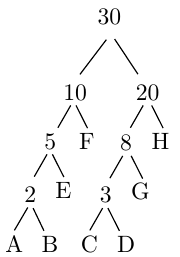
\includegraphics[width=0.15\textwidth]{huffmanTree.png}
 \caption{Sample of a completed Huffman-coding binary tree \cite[p. 70]{salomon2004data}}
 \label{HUFFMAN}
\end{mdframed}
\end{figure}

Instead of assigning variable, \textit{integral}, length codes per symbol as is done by Huffman coding, Arithmetic coding encodes an entire message as a sub-interval of [0,1). As with
Huffman a probability distribution has to be determined (or be specified) before the algorithm can be executed. The initial interval [0,1) is reduced by each consecutive 
symbol. The length of the sub-interval is proportional to the probability of occurrence of the symbol being read. The final symbol gets assigned any value inside the remaining 
sub-interval. As the interval decreases the number of bits required to encode each consecutive interval increases. However, the average number of bits needed to store 
each symbol is closer to the that of the entropy encoding of the dataset, since this average number can be \textit{real} value, unlike that of the per-symbol encoding of Huffman \cite[ch. 2]{salomon2004data}.

Both approaches lead to variable-size codes and both techniques have adaptive versions, which are useful in situations where the probability distributions change or have to be estimated. 
This approach is also applicable to the situation where the symbol table has to be computed on the fly, because it is impossible to perform multiple passes over data. This can, for example,
happen when processing streaming data and all compression has to be completed on the fly. Arithmetic coding achieves higher compression ratios in both adaptive and non-adaptive cases 
when compared to Huffman coding. It should be pointed out that the decompression step of Arithmetic coding is slow and unsuitable for cases where fast access is 
required \cite{ray1995database,williams1999compressing}\cite[ch. 2]{salomon2004data}.

\subsubsection{Transforms}
As the name suggest it can be useful to transform a dataset from one form to another in order to exploit its features for the purposes of compression. Such transformations 
includes, for example, wavelet transforms. A wavelet is a small, wave-like, function that is only non-zero over a very small domain and is useful
to separate the low frequency components from the high frequency components of, for example, an image. JPEG2000 and DjVu are popular formats that use 
wavelet transforms. The dataset is generally sampled at increasing frequencies to produce a series of representations that gradually increases in resolution. When added together 
these representations will reconstruct the original dataset. A sample of the Discrete Cosine Transform of an image (as employed by JPEG2000) is shown in figure~\ref{TRANSFORM_SAMPLE}. 
Only the transformation coefficients have to be stored in order to reconstruct each value in this series. The coefficients within this transformation can then be further compressed 
using other techniques, for example, Huffman coding and Run-Length Encoding (as is done in JPEG2000). If lossy compression (loss of accuracy which cannot be recovered after 
decompression) is tolerable, quantization can be used to discard unimportant values (for example the high frequency features of an image) \cite{952804}\cite[ch. 5]{salomon2004data}.
\begin{figure}[h!]
\begin{mdframed}
 \centering
 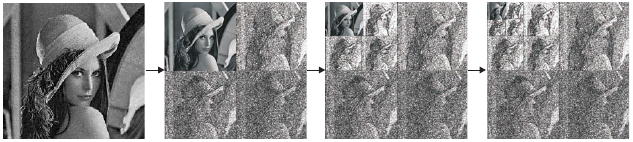
\includegraphics[width=1.0\textwidth]{DCTSample.png}
 \caption{Sample output from a Discrete Cosine Transform employed by JPEG2000 \cite{952804}}
 \label{TRANSFORM_SAMPLE}
\end{mdframed}
\end{figure}

Transforms are furthermore particularly useful where multiple levels of detail are desired. An example of this may include the transfer of scientific data over a network 
for real-time analysis and observation. Low resolution samples can be consistently transferred, while higher resolution samples can be transferred upon request \cite{Tao:1994:PTS:951087.951108}.
\subsection{Overview of predictive compression}
Previous research \cite{1607248,4589203,engelson2000lossless,lindstrom2006fast,O'Neil:2011:FDC:1964179.1964189,4976448,CGF:CGF681} in this area has yielded good results both in terms of compression ratio and speed. 
The common line of thought is to predict successive values with reasonable precision. Depending on the accuracy of the prediction, the difference between the predicted and actual value will be much smaller than the actual value itself. 
This difference can then be encoded using fewer bytes/bits of data (depending if compression occurs at a byte or bit level) by compressing the leading zeros after either an XOR or integer subtraction 
operation. Machine instructions to count the leading zeros can be found on AMD, newer Intel Processors and CUDA architectures. The leading zero count is then encoded as a prefix stream while the remaining bits/bytes 
are encoded as a residual stream.

Previous research suggests several different constructions of predictors. The use of a \textit{Lorenzo} predictor \cite{lindstrom2006fast,CGF:CGF681} generalizes the well known parallelogram predictor. 
The Lorenzo predictor extends the parallelogram to arbitrary dimensions. More detail on the parallelogram predictor will be given
in the implementation section, but it is useful to note that this approach is particularly useful for compressing large meshes. Other approaches include the use of prediction history 
(via a simple lookup table construction) as suggested by Burtscher et al. \cite{1607248,4589203,4976448}. Burtscher et al. reports a throughput of up to 670 MiB/s on a CPU implementation of their FPC 
compressor. An even simpler scheme by O'Neil et al. \cite{O'Neil:2011:FDC:1964179.1964189} reportedly achieved throughputs of up to 75GiB/s for compression and up to 90GiB/s 
decompression, implemented in CUDA. In this scheme only the difference between successive values are encoded (this will clearly only work if pairs of data points 
vary very little from one time step to the next). It is duly noted that the speeds achieved  are on the post-processing of results, already stored in graphics memory. 
The implementations by \cite{O'Neil:2011:FDC:1964179.1964189,1607248,4589203,4976448,engelson2000lossless} target 64-bit IEEE 754 
\textit{double} precision floating-point data.

The IEEE 754 standard of 2008 defines 3 interchange formats (32-bit, 64-bit and 128-bit). See figures~\ref{IEEE_FLOAT}~\&~\ref{IEEE_FLOAT_TAB}. Each of these have a common 
construction with the following subfields:
\begin{itemize}
 \item A 1-bit sign
 \item A w-bit length biased exponent
 \item A (d-1)-bit significand, where the leading bit of the significand is implicitly encoded in the exponent.
\end{itemize}
\begin{figure}[h!]
  \begin{mdframed}
  \centering
  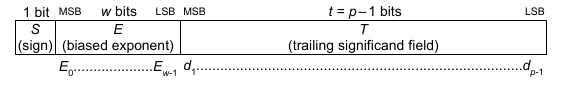
\includegraphics[width=0.6\textwidth]{IEEEinterchangeFormat.png}
  \caption{IEEE Interchange floating-point format \cite{4610935}}
  \label{IEEE_FLOAT}
  \end{mdframed}
\end{figure}
\begin{figure}[h!]
\begin{mdframed}
\centering
\begin{tabular}{|c|c|c|}
 \hline
 Precision & Exponent width & Significant precision \\
 \hline
 32-bit & 8 bits & 23 bits \\
 \hline
 64-bit & 11 bits & 52 bits \\
 \hline
\end{tabular}
\caption{Specifications for the 32-bit and 64-bit interchange formats}
 \label{IEEE_FLOAT_TAB}
\end{mdframed}
\end{figure}
The primary scheme proposed in this paper takes its inspiration from the work of O'Neil et al. \cite{O'Neil:2011:FDC:1964179.1964189}, but will operate on 32-bit 
IEEE 754 \textit{single} precision floating-point values, as pointed out in the introduction. The uncompressed data itself is also structured slightly 
differently to the model used by O'Neil et al. Instead of compressing each consecutive value the proposed compressor will operate 
over consecutive time slices (refer to figure~\ref{MeerKAT_PIPELINE}).

As pointed out in previous research \cite{engelson2000lossless,lindstrom2006fast} using floating-point operations in the prediction step can cause an irreversible loss of information due to floating-point
rounding errors. A simple alternative approach is proposed by Engelson et al. \cite{engelson2000lossless}: floating-point memory is simply treated as integer memory and all operations performed on that memory are integer operations. This
approach ensures the predictive scheme achieves lossless compression. In light of this only schemes that conform to this approach will be considered. Engelson et al. gives an example of how floating-point numbers
can be treated with integer operations. Figure~\ref{INT_REP} shows that if two floating-point numbers are relatively close to each other (in terms of magnitude) it is possible to discard some repeated bytes of information after performing 
an XOR operation to extract the remaining, seemingly random, residual bits. Therefore if an accurate prediction can be made for consecutive numbers a reasonable
saving in terms of compression ratio can be made. An XOR operation is a \textit{binary} operation (taking two operands). It returns false if both operands are the same. If $\oplus$ represents the XOR operation then 
inversion can be achieved as follows: $A\oplus B = C \implies (C\oplus A = B) \wedge (C\oplus B = A)$. The XOR operation is furthermore commutative, meaning: $A\oplus B = B\oplus A$. The inversion property is obviously critical 
to achieve decompression since the difference can be XORed with the observation at time $t-1$ to obtain the observation at time \textit{t}.
\begin{figure}[h!]
\begin{mdframed}
\centering
\begin{tabular}{|c|c|c|c|}
 \hline
  & & byte & 1\hspace{8 pt}2\hspace{8 pt}3\hspace{8 pt}4\hspace{8 pt}5\hspace{8 pt}6\hspace{8 pt}7\hspace{8 pt}8\\
 \hline
 $a_{1}$ & 2.3667\textbf{1}76745585676 & $\Rightarrow$ & 40 02 ef \textbf{09 ad 18 c0 f6} \\
 \hline
 $a_{2}$ & 2.3667\textbf{2}76745585676 & $\Rightarrow$ & 40 02 ef \textbf{0e eb 46 23 2f} \\
 \hline
 $a_{3}$ & 2.3667\textbf{3}76745585676 & $\Rightarrow$ & 40 02 ef \textbf{14 29 73 85 6a} \\
 \hline
\end{tabular}
\caption{Treating 64-bit IEEE 754 double precision floating-points as integer memory \cite{engelson2000lossless}}
 \label{INT_REP}
\end{mdframed}
\end{figure}
\section{Design and Methodology}
\subsection{Overview}
In light of the research questions and the limited scope of this report, focus will be placed on the usefulness of a predictive data compression 
step in the context of the MeerKAT project. This will be limited to an investigation on whether the algorithm can operate at the desired line rate of
40 GBit/s and whether it provides reasonable compression ratios. This initial investigation precludes the implementation of the algorithm as part of 
the networking stack employed in the KAT-7 pipeline. Reasonable compression in this context means achieving compression ratios, comparable to industry standard 
tools like GZIP and BZIP2. The possibility of using alternative predictive schemes to trade some throughput for a better compression ratio will also be investigated.
Such alternative schemes will include the following (notes on their efficient implementation will be provided in the implementation section):
\begin{enumerate}
 \item A Lagrange polynomial extrapolation.
 \item A parallelogram predictor.
 \item Moving mean \& median predictors.
\end{enumerate}
The key success criteria for this investigation are the following:
\begin{enumerate}
 \item Throughput in excess of 40 GBit/s is achieved by both the compressor and decompressor.
 \item Effective compression ratios, comparable to those achieved by GZIP and BZIP2 are achieved.
\end{enumerate}
\subsection{Packing algorithm}
The compacting algorithm being proposed is based on the approach taken by O'Neil et al. \cite{O'Neil:2011:FDC:1964179.1964189}. The algorithm is almost \textit{symmetrical} in its compression and 
decompression stages. In this context symmetry means the algorithm is executed in the opposite direction when performing decompression. The primary difference is that the leading 
zero count does not have to be computed for each element being decompressed. Refer to figure~\ref{PACKING_ALGORITHM} for more details.
\begin{figure}[h!]
\begin{mdframed}
 \centering
 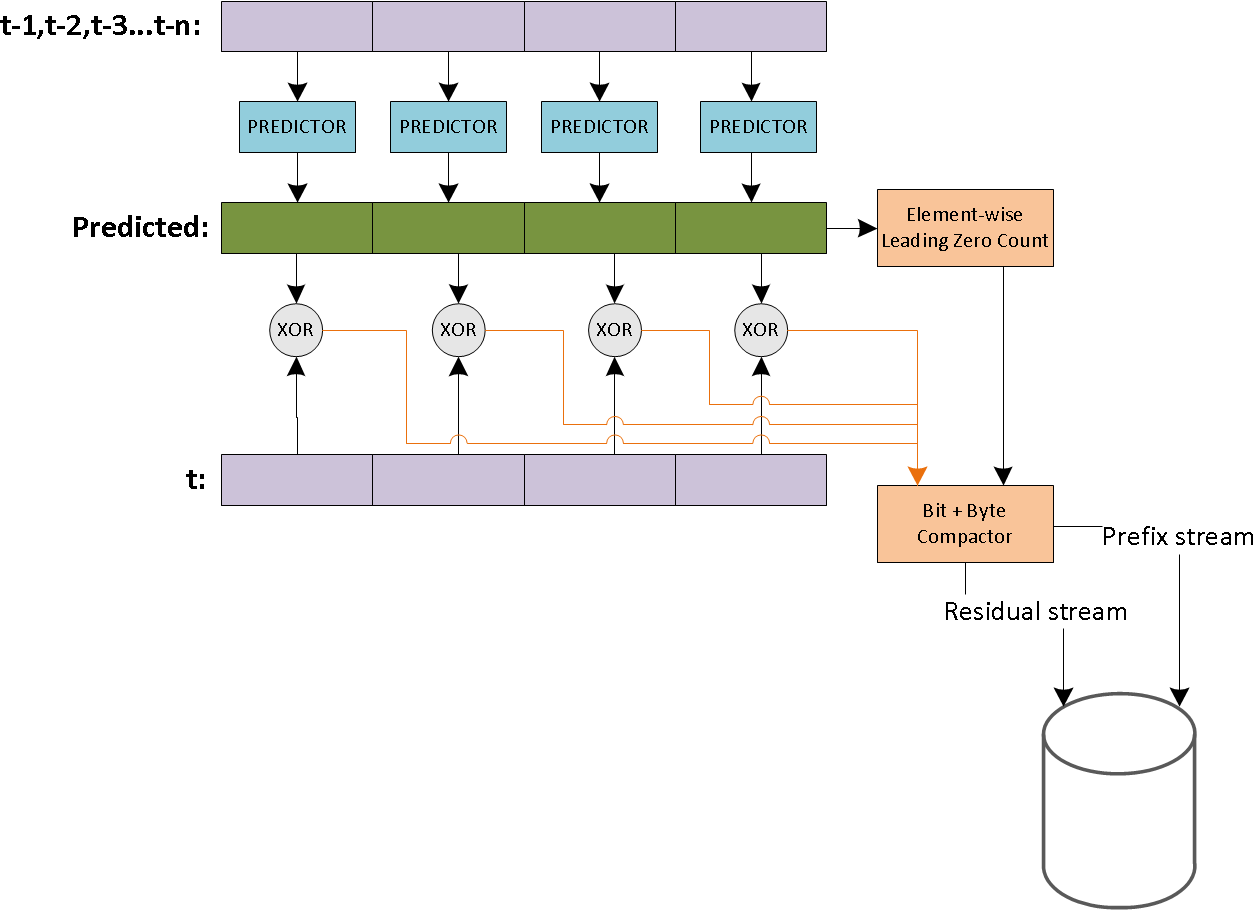
\includegraphics[width=0.7\textwidth]{Thesis_Alg.png}
 \caption{Prediction and compaction process}
 \label{PACKING_ALGORITHM}
\end{mdframed}
\end{figure}
The construction of the algorithm being specified in figure~\ref{PACKING_ALGORITHM} is used because it allows for easy swapping between different predictors. The predictor in this case 
can be any n-element predictor. As mentioned earlier the predicted value is XORed with the actual value to get a residual which can be compacted at either bit or byte level. This 
compaction simply removes the leading zeros from each leading zero count and stores each residual as a fixed-length prefix count. The number of bits needed to store $n$ leading 
zeros can be calculated as $\lfloor\log_2n\rfloor+1$ bits where $n\in\mathbb{N}_{>0}$. It remains to find the residual compaction scheme that gives the best results: packing at 
bit or byte level. Although a bit-packing scheme can pack an arbitrary number of zeros it requires longer prefixes to store the leading zero counts. The opposite is true 
for byte-packing schemes. Since the prefixes are always short a bit-packing scheme is used to store these fixed-length codes. Basic pseudo code is given in the implementation section.

Suppose the following two (converted) float values have to be compacted (the left-most byte is the most significant byte):
\begin{center}
  \begin{verbatim}
    #1: 00000000 01100010 01101000 11001001
    #2: 00000000 00000000 11110001 11110010
  \end{verbatim}
\end{center}
In this scenario the compaction of the residuals is done at byte level and the prefixes are done at bit level (assume 3 bits are needed to store up to 4 bytes of leading zeros):
\begin{center}
  \begin{verbatim}
    RESIDUALS:
    01100010 01101000 11001001 11110001 
    11110010
    PREFIXES (VALUES ARE PADDED UP TO ENSURE ONLY COMPLETE BYTES ARE STORED):
    00101000
  \end{verbatim}
\end{center} 
\subsection{Parallelizing compression and decompression steps}
There are three ways this can be achieved: 
\begin{enumerate}
 \item Even though the residuals are of variable length it is possible to pack them in parallel. However, there is an additional overhead to \textit{both} the packing and 
 unpacking process, since this approach requires a \textit{prefix sum} to be computed for the array of element-wise leading zero counts as O'Neil et al. \cite{O'Neil:2011:FDC:1964179.1964189} 
 points out.
 
 A prefix sum (or \textit{scan}) can be defined on any binary associative operator, $\oplus$ over an ordered set with $I$ as its identity. If $A=[a_{0},a_{1},\dots,a_{n-1}]$ 
 is an ordered set then the prefix sum scan is defined as $scan(A):=[I,a_{0},(a_{0} \oplus a_{1}),\dots,(a_{0} \oplus a_{1} \oplus ... \oplus a_{n-2})]$. 
 
 In the context of the packing scheme proposed here, the prefix scan is defined over the normal integer addition operator. An example of this will be $scan[2,1,3,4] = [0,2,3,6]$ 
 under normal integer addition. The leading zero counts are saved to an array, \textit{A}, after which the scan operation is computed on the array. The accumulated values are 
 stored in place and hence the algorithm has a \textit{constant} memory overhead (uses no extra memory). Each index \textit{A}[\textit{i}] will therefore store the starting 
 position (in bits) of the residual of the $i^{th}$ element \cite{blelloch1990prefix}. 

 This scan operation can be computed in parallel. Blelloch suggests such an approach \cite{blelloch1990prefix}. The algorithm will be discussed in greater detail in the 
 implementation section. Additionally a work-efficient CUDA version of the algorithm is discussed in GPU Gems 3 \cite{harris2007parallel}. In this version the algorithm is 
 optimized to avoid \textit{bank conflicts} (see the section on GPU architecture) and has been shown to be up to 6 times faster than a sequential CPU implementation for large 
 arrays.
 
 After the indexes have been accumulated using the prefix sum algorithm it is easy to see how different threads can pack residuals at the correct positions. Both a bit and byte
 packing scheme will, however, require \textit{atomic} operations to ensure against the \textit{race condition} that arises when multiple threads write to the same memory 
 location simultaneously. This memory-level-synchronization mechanism adds additional overhead in terms of wasted machine clock cycles.
 \item Incoming data can also be separated into blocks, after which multiple of these blocks can be done in parallel (where each block is compressed/decompressed in serial). This overcomes the issue of 
 additional overheads arising due to computing prefix sums and using atomics. This approach may have a detrimental effect on the compression ratio since the length of the residual array of each block 
 has to be stored.
 \item A more fine-grained parallelization is possible using vectorized instructions. The various Intel SSE, Steaming SIMD (Single Instruction Multiple Data) instruction set extensions (up to version 4.2) provide
 the opportunity to perform 4 instructions (adds, multiplies, logarithms, rounding, etc.) simultaneously per core. However, the SSE instruction sets do not have any element-wise bit-shift operations. A combination 
 of the Intel SSE and AMD XOP instruction sets, will however, provide enough support to write the most of the algorithm using vector intrinsics. The XOP instruction set extends the SSE instruction set by adding these 
 operations as one of its primary features. Adding these instructions will, however, make the implementation dependent on the architecture of the underlying machine it is executed on (and therefore less portable). 
 If this approach is successful the vectorized code should be extended to use the latest Intel AVX 2 instruction set in which Intel introduces element-wise shift operations and offset-loading operations as part of 
 future work. The AVX family of instructions can compute up to 8 SIMD operations in parallel per core. All these vectorized instruction sets make use of a very limited number of 128- and 256-bit registers (SSE and 
 AVX respectively). It remains to be investigated whether it is worthwhile to implement the proposed packing algorithm using SSE and XOP instructions.
\end{enumerate}
\subsection{Porting the implementation to CUDA}
General Purpose programming using Graphics Processing Units (GPGPU) brings a host of associated challenges. These challenges arise primarily due to the widely differing architecture of GPUs if compared
with the classical architectures of Central Processing Units (CPUs). Refer to figure~\ref{FERMI_ARCH} for a detailed overview of the microchip die structure of a Nvidia Fermi generation GPU. 
However, each generation of GPUs have widely differing architectures, each making many architecture specific optimizations. Each generation, for instance, will have both a 
different ratio and configuration of arithmetic cores to floating-point and special operations cores, per group of processing \textit{CUDA cores}. These cores are also known as 
\textit{streaming multiprocessors} (SMs). Additionally each generation has widely differing memory controller layouts. These may determine how many \textit{warps} of threads can be executed, when 
the warps are swapped in/out, along with many other properties. Each SM is split into groups of threads which are executed in parallel (normally this is specified as 32 threads per warp). 
These groups of threads are executed in \emph{atomic} batches, for example this may be a half-warp of threads on a G80 GPU \cite{harris2007parallel}.

A basic CUDA implementation will be provided to see if doing compression as a post-processing step on signal data already loaded to GPU (as part of the current pipeline) is a 
feasible alternative to a regular multi-threaded CPU implementation. Adaquite use of shared memory (as figure~\ref{FERMI_ARCH} shows GPUs have very large L1 and L2 caches available per SM) 
will be made and the implementation will take adequate precaution to \textit{coalesce} memory accesses and to avoid \textit{bank conflicts} when possible. 

Coalesced memory accesses are made if a continuous chunk of memory is accessed by a half-warp of threads at the same time. Normally these accesses have to be made in a uniform pattern that is aligned perfectly
with the structure of global memory. Individual memory calls to global graphics memory is a very costly operation (and therefore random accesses have to be avoided). Coalesced accesses are made simultaneously by 
the memory controller. Such accesses retrieve / write memory in larger chunks, which counters the latency associated with such an access. 

In GPU architectures (at the very least with Nvidia cards) \emph{shared} memory is divided up into banks. When multiple threads (specifically a half-warp of threads) try to 
access the same bank of memory, the memory accesses will be made sequentially. The general approach to avoid such a situation is to add padding between blocks of shared memory.

More details will be provided in the implementation section, but it is clear that a combination of the approaches (1 \& 2) taken with the CPU version will be required to make 
adequate use of the GPU architecture. This proposed implementation will consider assigning a block of data to each SM, which will, in turn, process that block in parallel without 
regard to operations performed on other SMs. This ensures that no unnecessary overheads due to costly card-wide synchronization steps are introduced. Instead all atomic 
operations and synchronization steps will be performed per-SM only.
\begin{figure}[h!]
\begin{mdframed}
 \centering
 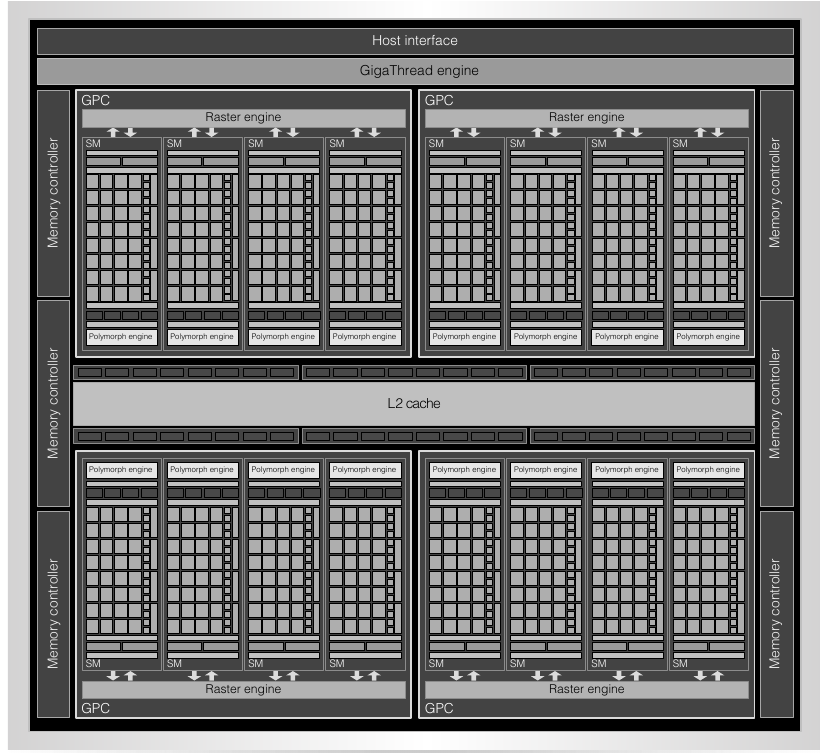
\includegraphics[width=0.8\textwidth]{fermi_arch.png}
 \caption{Architecture of the Fermi family of Nvidia GPUs \cite{wittenbrink2011fermi}}
 \label{FERMI_ARCH}
\end{mdframed}
\end{figure}
\subsection{Test data}
The correlated data is provided in the form of HDF5 files. Each of these files stores a three dimensional array of complex pairs. The first dimension is time. The second 
is signal frequency (as mentioned in the background section the telescope array will monitor a wide range of frequencies). The third dimension is a combination of two 
properties. Each number represents a correlation between two antennae. The antennae additionally have two modes of polarization (a horizontal and vertical polarization). 
The size of the last dimension is specified as two times the number of permutations of $n + 1$: $2\times((n+1)\mathbf{P}2)$ elements where $n$ is the number of
antennae in the array. The headers of the HDF5 files contain meta-information on the state of the telescope and what it is currently observing (this will determine the 
characteristics of the data itself as well as the range of frequencies being monitored). 

It should be noted that the headers cannot be compressed with the algorithm being proposed. An LZ variant / entropy encoder may be better tailored for this task. 
The headers vary between 13-14\% of the total h5 file size. However, the data is only written to these formats after it is received by the processing cluster (see 
figure~\ref{MeerKAT_PIPELINE}). Therefore if the algorithm being proposed is integrated into the front end of the pipeline as seen in figure~\ref{MeerKAT_PIPELINE} (as part of 
future work) it may still provide a significant saving in network I/O. 
\subsection{Structure and scope of the benchmarks}
Some of these HDF5 files measure more than 30GiB in size, each containing many timestamps (some spans over 4000 frequencies). It is reasonable to assume that once the number of correlations grow, emphasis will be placed on processing each 
time step (or portion thereof) as soon as it is received over the network. In future research the compressor may be integrated into the 7-layer OSI networking stack currently employed by the KAT-7 prototype. Due to the limited
scope of this project focus will be on analyzing the performance of the algorithms themselves and not to measure any disk I/O (except when comparing to other compression utilities for the sake of fairness).

This report will focus on the following analysis:
\begin{enumerate}
 \item A comparison between the a CPU implementation of the parallel (prefix sum-based algorithm) and the blocked approach (as specified previously) will be made.
 \item A detailed breakdown of how the algorithm performs on different numbers of cores (of whichever method is determined most fit in step 1) will be provided.
 \item The effectiveness of a parallelogram predictor, a Lagrange extrapolation predictor \cite{engelson2000lossless} and a moving mean and median scheme will be determined. 
       Each of these methods will be described in greater detail in the implementation chapter.
 \item The feasibility of implementation using the Intel SSE and AMD XOP vectorized instruction sets will be investigated.
 \item Benchmarks of the algorithm against the standard programs used for comparison: GZIP, BZIP2 and ZIP. In this case the disk I/O will be included for the sake of fairness.
 \item The feasibility of a CUDA implementation, as outlined earlier, will be determined.
 \item Finally results from concurrent research being conducted into entropy encoding and run-length encoding will be compared to those achieved in this investigation. This comparison will include a 
       breakdown of performance in terms of both throughput and compression ratios.
\end{enumerate}
\subsection{Benchmarking platform}
The benchmarking platform is designed with two primary software engineering goals in mind:
\begin{itemize}
 \item It should be as \textit{decoupled} as possible, making use of predefined interfaces. This will assist in providing several implementations of the CPU version (for example SSE, different linear predictors and different parallelization
 approaches) and simply swapping one implementation for another. Interactions between components must be kept to a minimum.
 \item The components must be \textit{cohesive}: they should contain only relevant operations and should be considered as atomic units.
\end{itemize}
The architecture described in figure~\ref{TOOL_ARCH} is used for the benchmarking platform. All the external dependencies depicted in the component model is freely available
and are actively maintained. There is no considerable technical risk in using these libraries. Technical details will be provided in the next section. The 
benchmark process is relatively simple and its flow is depicted in figure~\ref{TOOL_FLOW}.
\begin{figure}[h!]
\begin{mdframed}
 \centering
 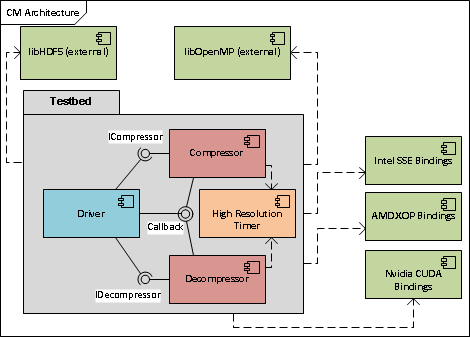
\includegraphics[width=0.6\textwidth]{Thesis_Arc.png}
 \caption{Architecture of the loosely coupled benchmarking platform, including external library dependencies}
 \label{TOOL_ARCH}
\end{mdframed}
\end{figure}
\begin{figure}[h!]
\begin{mdframed}
 \centering
 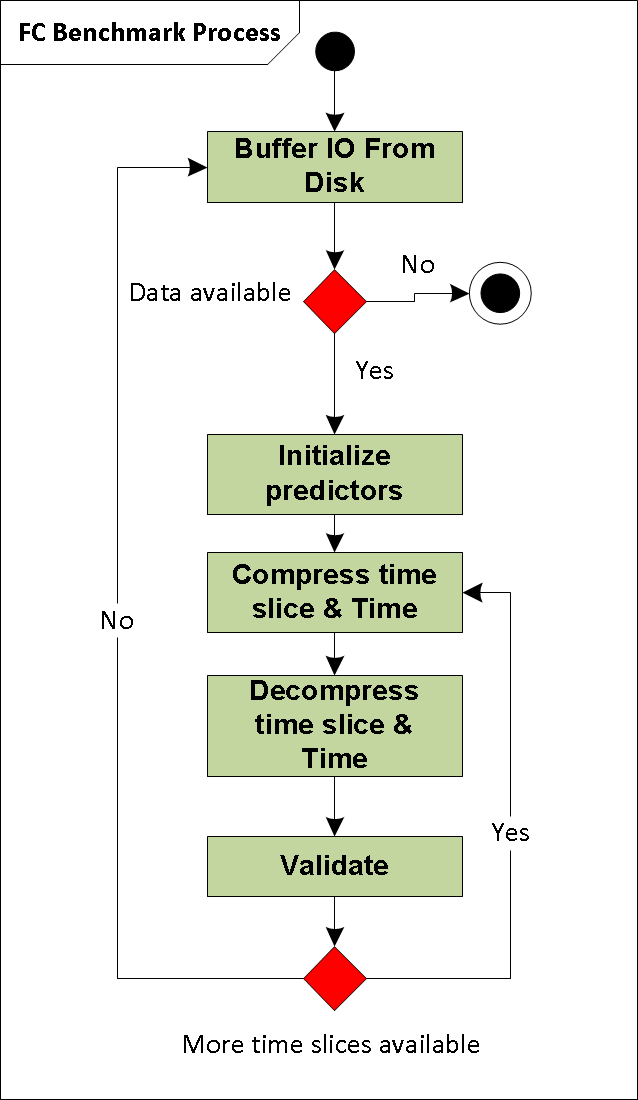
\includegraphics[width=0.25\textwidth]{Thesis_Flow.png}
 \caption{Behavioral model of the benchmarking platform}
 \label{TOOL_FLOW}
\end{mdframed}
\end{figure}
\section{Implementation}
 \subsection{Basic algorithm}
  In order to give a more detailed description to the algorithm illustrated in figure~\ref{PACKING_ALGORITHM} in the previous section, the pseudo code for the compaction
  process is given below:
\begin{verbatim}
SUBROUTINE Compact(FLOAT[] data, UNSIGNED INT32 numElements, 
		    out UNSIGNED INT32[] residuals, 
		    out UNSIGNED INT32[] prefixes)
	 //ASSUMPTION: 3 BITS NEEDED TO STORE UP TO 4 BYTES OF LEADING ZEROS
	 //ASSUMPTION: COMPACTION IS DONE INTO 32 BIT INTEGER ARRAY
BEGIN
	 UNSIGNED INT32 bitPosInResidualArray = 0
	 FOR index = 0 TO numElements - 1 DO
		  /*
		  This prediction step requires up to "n" arrays of the 
		  same size of "data".
		  */
		  UNSIGNED INT32 predictedValue = linearPredict(index) 
		  UNSIGNED INT8 leadingZeroCount = clz(data[index])
		  UNSIGNED INT32 difference = predictedValue XOR data[index]
		  //save the prefix:
		  prefixes[index*3 INT_DIV 32] = SHIFT (leadingZeroCount INT_DIV 8) to \\
		    the index*3 MODULO 32 th bit
		  IF there are remaining bits that couldn't be fitted THEN
		    prefixes[index*3 INT_DIV 32 + 1] = SHIFT remaining bits that couldn't \\
		      be fitted in the previous operation to the first bit of the next byte
		  END IF
		  //save the residual:
		  residuals[bitPosInResidualArray INT_DIV 32] = SHIFT difference to \\
		    the bitPosInResidualArray MODULO 32 th bit
		  IF there are remaining bits that couldn't be fitted THEN
		    residuals[bitPosInResidualArray INT_DIV 32 + 1] = SHIFT remaining bits \\
		      that couldn't be fitted in the previous operation to the first bit \\
		      of the next byte
		  END IF  
		  //increment position in the residual array
		  bitPosInResidualArray += leadingZeroCount
	 END FOR
END SUBROUTINE 
\end{verbatim}
The decompression algorithm is remarkably similar, except that the leading zero count is not computed, but is instead retrieved from the prefix array. The shift
operations are inverted to retrieve the bits (that may be splitted over two consecutive elements) in both the prefix and residual arrays. The prediction step is moved towards
the end of the routine, where the predicted value is XORed with the residual to restore the original, uncompressed, value.
  \subsection{Notes on fault tolerance and error propagation}
    Due to the fact that the reconstruction of each observation at time \textit{t} depends on the preciding, corresponding, observation at time $t-1$, which in turn 
    depends on the corresponding observation at time $t-2$, error propagation will become a problem in a production environment (especially if network transmission uses a transport
    protocol without integrity checking, like UDP). 
  
    If one of the residuals becomes corrupted (either through network error or disk corruption) each subsequent, corresponding, 
    observation will be decoded to the wrong value. Since multiple observations can be stored into a single 32-bit store the observations in the immediate vacinity of the corrupted
    store (and their successors) will be affected. On the other hand if one (or more) of the prefixes becomes corrupted, all the residuals after the first corrupted prefix, $P[c]$ will be decoded 
    incorrectly as well. This is due to the fact that the accumulated prefix count over $P[0]\dots P[c]\dots P[m]$ are used to reconstruct the residual at index \textit{m}. These 
    errors will continue to propagate until a fresh initialization is done on both the compressor and decompressor. 
    
    In a production environment it will be necessary to include integrity checks using a \textit{checksum} algorithm like the Merkle Damgard 5 (MD5) message digest, in order to validate output after all the observations
    at time \textit{t} have been decoded. A message digest algorithm is simply a function that takes an arbitrary length input, \textit{M} and maps it to a fixed length output, 
    \textit{N}. Any slight change in the input, $M'$ will result in a substantially different output, $N'$. The chances of a collision ($N = N'$) are very slim, meaning that 
    the checksum provides a viable way of checking archive integrity. A checksum produced by MD5 is only 128 bits long and will not have a significant detremental impact on the
    compression ratio, since it only has to be saved for the entire set of observations at time \textit{t} and not per block. Any errors can be mitigated by ensuring that the 
    compressor and decompressor is reinitialized regularly.
 \subsection{Alternative linear prediction schemes}
  The most basic prediction scheme simply encodes the difference between observations at time \textit{t} and $t+1$. This difference is given as $O[t]$ xor $O[t-1]$. The 
  downside to this basic predictor is that it is particularly sensitive to the structure of the underlying data. It will only work if \emph{most} consecutive values varies 
  slowly over time. Using an n-element predictor may help mitigate the effects of noise. However, as pointed out earlier: any operations over these n-elements have to be integer 
  operations and not floating point operations, due to the rounding errors they may introduce (as pointed out in the background section). All floating-point memory are therefore 
  cast to integer-typed memory before values are retrieved.
  
  These predictions, however, still have to be fast and preferably have an average linear computational complexity, $\theta(n)$. The predictor will only 
  store the previous \textit{n} observations in a fixed-length queue. This implies that the memory overhead for the predictor is $n\times m$ where \textit{m} is 
  the total number of elements being processed at time $t$.
 \subsubsection{Lorenzo predictor}
 The n-dimensional Lorenzo predictor is a generalization of the two dimensional parallelogram predictor (see figure~\ref{LORENZO}). It can be used to predict scalar 
 functions that are polynomials of degree $n - 1$ and has been proven useful in scalar field compression \cite{CGF:CGF681}. In each of the 3 cases below only simple
 integer additions and subtractions are needed: the sum of the values in red are subtracted from the sum of the values in green. In the two dimensional case this 
 addition and subtraction is known as the \textit{parallelogram rule}. The predicted value is computed from previous observations as as $P = O[t-1] + O[t-2] - O[t-3]$.
 The prediction operation remains simple and should not have a considerable impact on the overall throughput. However, this approach will still be quite sensitive to noise.
  \begin{figure}[h!]
  \begin{mdframed}
    \centering
    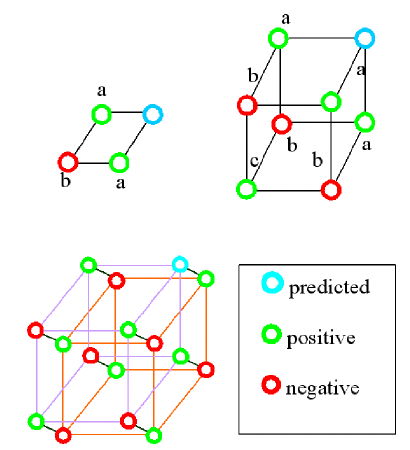
\includegraphics[width=0.3\textwidth]{lorenzo.png}
    \caption{Lorenzo predictor for 2D (upper left), 3D (upper right) and 4D (lower left) data \cite{CGF:CGF681}}
    \label{LORENZO}
  \end{mdframed}
  \end{figure} 
 \subsubsection{Moving average and moving mean}
  An integer-based moving mean is simple to implement and involves only a summation and an integer division (and therefore clearly has a linear computational complexity).
  However, the mean of a sample is sensitive to outliers, and therefore will not work well for noisy data. A simple solution will be to use a median based scheme
  where the predicted value is the center value of a \textit{sorted} list of observations. However, a naive implementation of such a median-based scheme will
  be slow due to the overheads of sorting. Wirth suggests an algorithm \cite{wirth76} to select the median using a basic \textit{pivoting} scheme in $\theta(n)$
  time. A pivot divides a dataset into two groups. The elements in the group to the right of the pivot are larger than the pivot and the elements in the group to
  the left of the pivot are smaller (or equal) to the pivot. The two groups do \emph{not} necessarily have to be ordered. The median is chosen through the following
  method that selects the \textit{k-th largest value} \cite{wirth76}:
  \begin{verbatim}
FUNCTION INT32 pivotMedian(INT32[] data, int n) {
    INT32 i, j, l, m, k = n/2-1 //k is the kth largest element in the array
    INT32 x, s

    l=0 //lower bound
    m=n-1 //upper bound
    WHILE l<m DO //swap elements in group L and M until the two indexers cross
        x=data[k]
        i=l
        j=m
        REPEAT
	    //find 1 element in each sub-array that has to be swapped
	    //to the other sub-array:
            WHILE data[i]<x DO i++
            WHILE x<data[j] DO j--
            IF i<=j THEN
		    //swap:
                s=data[i]
                data[i]=data[j]
                data[j]=s
                i++
                j--
            END IF
        WHILE i<=j
        if(j<k) l=i
        if(k<i) m=j
    END WHILE
    RETURN data[k] //mid-point in the array
}
  \end{verbatim}
 \subsubsection{Lagrange prediction}
  Lagrange extrapolation prediction is a gradient-based method that can be used to predict a value of a polynomial at $t+1$, given the values at $t\dots t-n$.
  The method is commonly used for interpolation between known points on a curve, defined by some polynomial. Good extrapolations are only possible for 
  \textit{smooth} data.
  
  If a function $f:[1\dots n] \rightarrow \mathbb{R}$ is evaluated over a time interval $[1\dots n]$ and its results stored as a sequence of values 
  $a_{1}\dots a_{n}$ where $a_{i} = f(i)$, then such a sequence is called \textit{smooth of order m} if for all $j>m$, $a_{j}$ can be approximated with reasonable
  accuracy from extrapolating from the previous \textit{m} values. Such smooth sequences normally arise as solutions of ordinary differential equations (ODEs) in
  simulation models \cite{engelson2000lossless}.
  
  The model implemented in this report uses \textit{fixed-step extrapolation} (the time between consecutive observations is assumed to be of constant duration), but
  the method works just as well if these differences vary in length, as long as the underlying sequence can be approximated some polynomial \cite{engelson2000lossless}. 
  The method builds from \textit{Lagrange's Rule}. It states, that for a given function, $f$ implicitly defined over the previous \textit{m} 
  observed values, given some extrapolation points, indexed by $x\in I = \{i\in\mathbb{N}|i\geq 0\wedge i\leq m\}$ there exists some polynomial, $\varphi_{m}$ such that 
  $(\forall x\in I) \varphi_{m}(x)=f(x)$. The polynomial is defined as $\varphi_{m}(x^{*})=\sum_{x\in I}L_{x}(x^{*})f(x)$ where each coefficient, $L_{x}(x^{*})$ 
  can be computed by the equation below. Note that $x^{*} = m + 1$, the index of the unknown value of \textit{f}, after the $1\dots m$ previously observed values.
  \begin{equation}
   L_{x}(x^{*}) = \prod_{k\in{I},k\neq x}\left(\frac{x^{*}-k}{x-k}\right)
  \end{equation}

 \subsection{Algorithm parallelization and its implications for GPGPU architectures}
  As pointed out in the design section the parallelization of the basic algorithm discussed earlier can be done by dividing incoming data up into fixed size chunks after which 
  multiple blocks can be packed in parallel. This approach is detrimental to the compression ratio, since the size of each
  block's residual stream has to be stored (this effect will be worse if there are a large number of blocks). The approach is relatively straightforward to 
  implement and does not modify the structure of the basic algorithm at all.
  
  The alternative approach is to convert the basic algorithm into an element-wise parallel algorithm. As mentioned in the design chapter this requires a prefix sum to be computed 
  in order to obtain the starting position of each residual in the residual stream. The prefix scan is a trivial case of a dynamic programming problem and the algorithm 
  \cite{blelloch1990prefix} is shown below:
  \begin{verbatim}
   SUBROUTINE scan(out INT32[] out, INT32[] in)
    INT32 i = 0
    INT32 sum = in[0]
    out[0] = sum;
    WHILE i < length(in) DO
      ++i
      sum += in[i]
      out[i] = sum
    END WHILE
   END SUBROUTINE
  \end{verbatim}
  Blelloch suggests a novel approach \cite{blelloch1990prefix} to compute this prefix scan in parallel. The algorithm requires the size of the input array to
  be a power of 2. If this is not the case padding has to be added to the input array. There are three primary steps to the algorithm, with a synchronization point between each. First
  an \textit{up-sweep} operation is completed, then the last element is set to 0, and finally a \textit{down-sweep} operation is completed. Both the \textit{up-sweep} and \textit{down-sweep} operations
  can be respresented by a \textit{complete} binary tree of $\log_2n$ levels (meaning that each level is fully filled). Each level of the tree can be done in parallel and therefore the algorithm has a 
  complexity of $O(n/p + \log_2{p})$ where \textit{p} is the number of processors in a system. The \textit{up-sweep} and \textit{down-sweep} operations (using integer addition) over a short sequence of integers is shown
  in figure~\ref{PARALLEL_SCAN}.
  \begin{figure}[h!]
  \begin{mdframed}
    \centering
    \begin{subfigure}[b]{0.8\textwidth}
      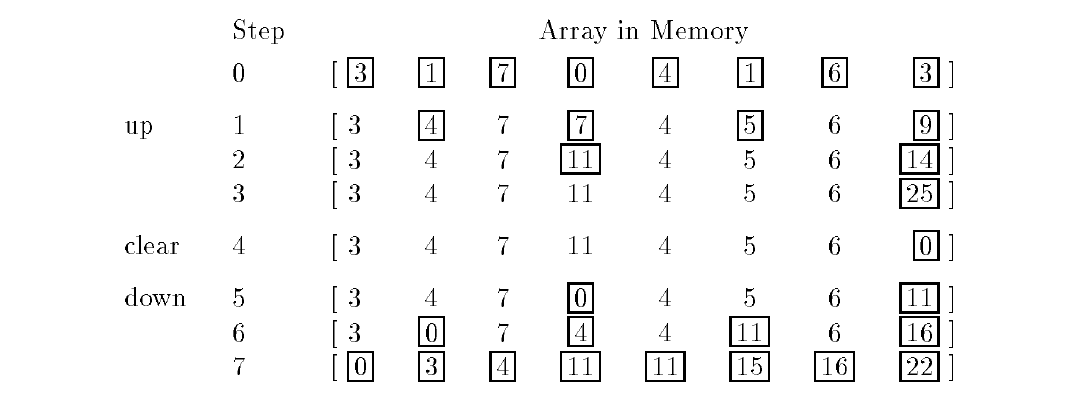
\includegraphics[width=0.9\textwidth]{scanOperationOnArray.png}
      \caption{Steps of the scan operation being executed in order on the sequence [3 1 7 0 4 1 6 3]}
      \label{UPSWEEP_DOWNSWEEP}
    \end{subfigure}
    \begin{subfigure}[b]{\textwidth}
      \centering
      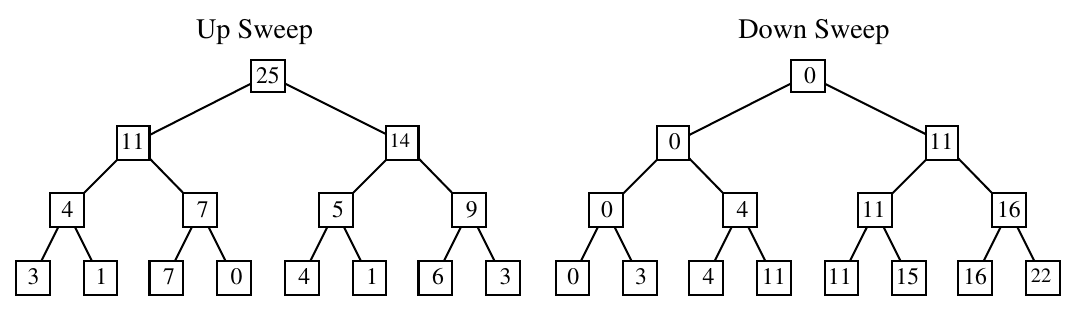
\includegraphics[width=0.7\textwidth]{upsweep_downsweep.png}
      \begin{minipage}{\textwidth}
        \begin{verbatim}
//UP-SWEEP:
  FOR d from 0 TO log2(length(A))-1 DO
    FOR i from 0 TO length(A) - 1 IN STEPS OF POW(2,d+1) IN PARALLLEL DO
      A[i + pow(2,d+1) - 1] += A[i + pow(2,d) - 1]
    END FOR
  END FOR
//DOWN-SWEEP:
  A[length(A)-1] = 0
  FOR d from log2(length(A))-1 DOWNTO 0 DO
    FOR i from 0 TO length(A) - 1 IN STEPS OF POW(2,d+1) IN PARALLLEL DO
      INT32 temp = A[i + pow(2,d) - 1]
      A[i + pow(2,d) - 1] = A[i + pow(2,d+1) - 1] //set left child
      A[i + pow(2,d+1) - 1] += temp //set right child
    END FOR
  END FOR
//EFFICIENCY NOTE: Powers of 2 are efficiently implemented as:
POW(2,n) = (2 << n-1) //where "<<" is the arithmetic left-shift operator
//and n is strictly greater than 0
        \end{verbatim}       
      \end{minipage}
      \caption{Tree representations with respective algorithms to compute each level in parallel (for both up- and down-sweeps)}
      \label{PARALLEL_SCAN_SUB_ALGORITHMS}
    \end{subfigure}
    \caption{Parrallel scan algorithm example and pseudo code \cite{blelloch1990prefix}}
    \label{PARALLEL_SCAN}
  \end{mdframed}
  \end{figure}
 
 The entire algorithm can now be turned into three steps that can each be computed in parallel:
 \begin{enumerate}
  \item Perform a leading zero count and store the prefixes as discussed in the basic pseudo code, but store the leading zero count to an array, A. The prefixes are fixed in length, so placing them
  into the prefix stream in parallel does not pose a problem.
  \item Compute $B = scan(A)$ in parallel
  \item Each element, $B[i]$ is now the stating position (in bits) of the residual of element $D[i]$. This means the variable-length residuals can be placed into the residual stream in parallel.
 \end{enumerate}
 
 The algorithm shown in figure~\ref{PARALLEL_SCAN} assumes execution takes place in a \textit{shared-memory} architecture, where each processor has access to the memory of the other processors and that synchronization
 can take place across multiple processors. In CUDA the last condition is not easily met: the global synchronization required by the parallel prefix sum scan can only be achieved through a global memory barrier. 
 However, this will cause a high number of context switches for every SM on the GPU (especially if the number of blocks are much larger than the number of available SMs). The alternative approach is to let each SM
 compute the prefix sum of a sub-sequence of numbers and store its last value of the accumulation as $S_{i}$. Each block total, $S_{i}$ is then distributed to the $i+1\dots n$ blocks of sub-sequence prefix sums in 
 parallel \cite{harris2007parallel}.
 
 The last, distribution, step adds additional overhead to the parallel algorithm. Instead, the dataset can be split into blocks that is a multiple of the warp size in length. This means that the data can be
 spread throughout the entire GPU to achieve a high \textit{occupancy} of the available SMs. Each SM then packs its block in parallel by computing a short prefix sum only for leading zero counts of the block 
 it is processing. 
 
 If this approach is taken in conjunction with the modifications described in GPU Gems 3 \cite{harris2007parallel}, a fast, work-efficient, parallel prefix sum scan can be implemented, that both minimizes overheads, and 
 includes optimizations through the use of shared memory on the GPU. These modifications includes adding padding  to each shared memory index according to the \textit{degree} of the bank conflict at the associated 
 depth of the indexing tree shown in figure~\ref{PARALLEL_SCAN_SUB_ALGORITHMS}, and letting each thread compute two values at a time. By doubling the strides between each successive level in the tree, the modifications 
 ensures that double the number of threads can be executed on that level without bank conflicts. 
 
 The next complication for an element-wise packing implementation is the matter of atomic operations. This issue arises due to sharing an atomic memory location between multiple threads that require simultaneous access
 to that location. The following example illustrates a race condition between 2 threads, packing residuals into a 32-bit residual array: thread 0 tries to pack 00000000 00000000 00011101 01100111 into residual store 
 $R[0]$ while thread 2 tries to split 00000000 01001010 01110001 01111111 into the same $R[0]$ and its successor, $R[1]$. Since $R[0]$ can only be written to by one thread at a time, either thread 1 will overwrite what has
 been written by thread 0, or the converse. This clearly causes irreversible loss of data. One way to avoid this is to lock the memory location for reading and writing while another thread is reading and writing to the 
 location. This potentially serializes the memory access.
 
 One way to avoid two atomic operations per residual is to use an array of bytes as the atomic units of the residual stream. However, since each element is 4 bytes in length, there may be anything from 0 up to 4 global memory
 write operations, along with the necessary control logic that will result in \textit{branch-diversion}. In the context of general GPU architecture this has potentially devastating consequences for simultaneous execution. As mentioned
 earlier each SM consists of many arithmetic units that are executed in atomic groups (each performing the same basic instruction). When some threads are required to perform one task while the others have to perform another the
 SM is forced to let all the threads perform both tasks in sequence, each time discarding values from the threads that are not supposed to execute through a masking operation. This means that double the number of clock cycles are needed
 to perform a branch. This problem becomes worse if a 3- or 4-way branch is necessary. This branch-diversion, coupled with multiple costly memory accesses may prove worse than using an atomic operation. 
 
 Additionally, it is possible to remove the atomic operations from the prefix compaction operation by storing only prefixes with a length that divides the length of the closest atomic unit (byte, short or integer). If the compacting 
 operation is constrained to packing up to 3 leading zero bytes of residuals, only 2 bits are needed to store this count per element. Every $16^{th}$ thread then has to compute 16 leading zero counts and store them simultaneously 
 into a single 32-bit prefix store. In order to avoid multiple write operations to global memory the 16 prefixes can be stored into a register before a call to global memory is made.
 \subsection{Feasibility analysis}
  \subsubsection{Compression feasibility}
  As mentioned previously the packing of residuals can be done at either bit or byte level. When packing at a bit level $\lfloor\log_2n\rfloor + 1$ bits are needed to represent
  \textit{n} leading zeros. When packing up to 31 leading zeros 5 bits are needed whereas 3 bytes of leading zeros can be packed using only 2 bits for each prefix as explained earlier. Which scheme
  works better is entirely dependent on the properties of the data and how accurate the predictions are. From experimentation, packing at byte level (up to 3 bytes of leading zeros) is the most 
  efficient scheme. It gives compression ratios approximately 1\% better than the closest bit-level packing scheme. The compression ratios achieved when encoding the
  difference between successive observations (by means of an XOR operation) are not very high. Depending on the dataset compression ratios of between 92\% and 93\% are observed. This shows that 
  although the compression scheme is rather basic there is some coherence between successive observations. 
  
  The ratios mentioned above includes storing the following information:
  \begin{itemize}
   \item All observations at time, $t=0$ are stored in their uncompressed form, along with the total number of values per time step. Both the compressor and decompressor are 
   initialized with this size and the values at this initial time step. When the number of observations changes (say due to a larger number of frequencies being sampled, both the
   compressor and decompressor have to be re-initialized.
   \item For the block-based approach the number of blocks must be stored if this value is not fixed by the implementation of the scheme.
   \item Since the residual arrays varies in length, the length of the residual array (per block if necessary) is stored before storing each block of residuals.
   \item The prefix array is stored without a length field, due to the fact that the prefix array size can be computed from the number of elements (per block if necessary).
  \end{itemize}
  The ratios, however, do not reflect additional header meta information (as found in the sample h5 files) and are solely based on the number of 32-bit floating-point values each
  h5 file contains. 
  \subsubsection{Parallelization approaches and optimizations on the CPU}
  The initial implementation considered parallelizing the algorithm at element level using prefix sums as described in the previous section. Even when using up to 16 CPU threads through OpenMP the overheads of computing a prefix 
  sum over all the elements turned out to be too costly on a CPU-based architecture. Although the implementation scaled roughly linear in throughput per core added it only managed to achieve compression throughputs of around 
  400 MiB/s and decompression throughputs of around 600 MiB/s on a 16 core test. This is a lot slower than the required throughput of 5 GiB/s. It is duely noted that the throughput rates achieved in the element-wise parallelization 
  includes several optimizations such as the removal of branches (for example branchless implementations of minimums and maximums are employed \footnote{Sean E. Anderson 
  provides several bittwiddled implementations of minimums, maximums and binary logarithms on his website: \url{graphics.stanford.edu/~seander/bithacks.html}. Last accessed: 3 
  October 2013} for the arithmetic bit shifting operations shown in the pseudo code), as well as the removal of some of the atomic operations as discussed in the previous sections.
  
  The failure of this approach in a CPU environment, however, does not necessarily preclude a similar approach being taken on a GPU. It has been shown \cite{harris2007parallel} that a 
  prefix sum can be computed up to six times faster on a GPU for large arrays of up to 16.7 million elements. This result, coupled with the fact that elements can be packed in a massively
  parallel environment is reason enough to investigate a CUDA implementation (more details on this can be found later in this chapter).
  
  The alternative approach to this element-wise parallel scheme, is to separate the data into blocks. There is one downside to this approach: it will degrade the compression
  ratio by a small amount depending on the number of blocks chosen (since the length of the residual array has to be stored). This approach proved more feasible than the 
  element-wise parallel packing. Using pthreads up to 0.673 GiB/s was achieved for the compression scheme and 1.178 GiB/s for the decompressor (using 16 cores). After replacing
  the p-threaded model with OpenMP a major breakthrough was made: the compressor achieved rates up to 1.98 GiB/s and the decompressor up to 3.66 GiB/s using 16 cores. Further 
  optimizations included using a leading zero count assembler instruction \footnote{\texttt{LZCNT rO,rI} is a machine instruction found on most AMD processors (since the 
  introduction of their XOP vector instruction set), as well as newer Intel processors. Nvidia GPUs have similar support for leading zero counts.} instead of loops to obtain 
  the count. This optimization increases the throughput by up to 200 MiB/s on a quad-core processor. When the implementation is run for large files on a 32 core AMD Opteron platform
  the desired throughput of 5 GiB/s is achieved. A detailed breakdown is given in the results section.
  \subsubsection{Alternative prediction schemes}
  The basic difference scheme discussed earlier will not work well in the case where the sign bit of 2 consecutive observations differs (as previously mentioned the sign bit is the most significant bit of an IEEE 754 
  floating point representation, implying that there will be no leading zeros to encode). A solution to this is to dedicate an extra bit per prefix in order to store the sign value. From experimentation it was determined that
  this trade-off between storing an extra bit for every prefix and the number of signed differences is not worth encoding: a saving of less than 0.01\% is made for a number of the sample datasets. 
  
  The next simple modification to the scheme is to test whether using normal integer subtraction fairs better than an XOR operation. Burtscher et al. points out that integer subtraction faired much worse both in terms of
  compression ratio and throughput for their FPC compressor operating on 64-bit floating points values \cite{4589203}. This is the same for the 32-bit KAT-7 being considered in this report. A loss of between 2\% to 3\% in 
  compression ratio is observed. It is therefore better to stick with a simple XOR operation.
  
  The integer mean predictor fairs poorly compared to the simple difference scheme by degrading the compression ratio by 3\% to almost 7\% (thereby inflating the data). The effect worsens when the number of prediction 
  steps are increased. As pointed out earlier such a mean scheme is prone to outliers (which can be expected in noisy data). The median scheme was expected to fair better as mentioned earlier and an implementation of the pivoting 
  scheme confirmed this suspicion. Compression ratios similar or slightly smaller (roughly 1\%) than the normal difference based scheme are observed, depending on the number of prediction steps being used. However, although the 
  pivoting algorithm discussed earlier has an average linear computational complexity, it does have a number of branches. This caries a severe penalty on throughput: over 
  71\% of the throughput is lost in the case of compression, while just short of 90\% is lost when decompressing. The effect worsens as the number of predictive steps are increased. In light of this result the median scheme is not
  a viable alternative to the basic difference scheme.
  
  The Lagrange predictor is accurate for smooth data (for example that of a sinusoid) that can be well approximated by some polynomial of degree \textit{n}. However, the noise present in the KAT-7 data renders this
  method of prediction unsuitable for the purposes of compression. Similar to the mean-based predictor, the scheme inflated the data when up to ten predictive steps were chosen. Similarly, the parallelogram predictor 
  also degraded the compression ratio by approximately 3\%.
  
  Other solutions not explored in this project include using a lookup table to store predictions. This approach is used in the FPC predictor mentioned earlier \cite{4589203}. The scheme is fast and reportedly achieves up to 
  1.36 GiB/s \cite{4976448} as a parallel implementation on a 3 Ghz Intel Xeon quad-core processor. This scheme uses the same block-based parallel approach investigated in this report. However, the primary concern with this 
  scheme is that, as the number of observed values grow, so does the size of the lookup table. This approach is therefore not as well-tailored towards a GPU implementation as the difference-based scheme investigated 
  in this report, because it will require more global memory accesses than a simple lookup of a single previous observation. It may be worthwhile to investigate whether a CPU implementation of FPC will work on the sample 
  data produced by the KAT-7 array in future work.
  \subsubsection{Vector intrinsics}
  The Intel Multimedia Extensions (MMX), SSE and AVX along with the original 3DNow, SSE extensions and XOP extensions added by AMD, forms a family of vectorized instruction sets which adds the ability to 
  perform a single instruction on multiple data elements of the same type in parallel. The original SSE instruction set added eight special 128-bit registers. The instruction set adds 
  the ability to perform both integer-arithmetic operations and floating-point operations on any continuous sequence of elements stored into these special registers. It imposes the special condition that the 
  elements loaded into a single register are all of the same bit-length (64,32,16 or 8-bit values).
  
  As the name suggests these special machine instructions are focussed on providing greater flexibility for performing a single instruction on multiple data. A good example of where
  a speedup can be expected is in parallelizing vector addition. However, in the case of implementing a packing algorithm the original SSE instructions are not sufficient since it only allows 
  bit-shifting multiple elements by the same amount. The packing algorithm requires that four 32-bit values each be shifted by a different amount. A simple solution is to employ the AMD XOP 
  instruction set which adds the ability to perform element-wise arithmetic bit shifting. The problem with this approach is that no Intel processor prior to the latest (at the time of writing) 
  Haswell series of processors support this operation through the AVX 2 extensions.
  
  The next major problem is that there is both a limited number of registers available and a packing algorithm does not have the same number of outputs as inputs. Altough
  the majority of the algorithm can be written as SSE and XOP instructions while the storage section can be written as as four separate instructions this avenue of research
  proved fruitless because of both the limited number of registers available and the overheads of employing both normal instructions and vectorized code (specifically conversion
  between the two). In both the compressor and decompressor the augmented code halves the throughput achieved before the SSE and XOP instructions were added. This finding precludes
  using the AVX 2 instruction set which adds several 256-bit registers (that can be used to perform 8 32-bit integer/floating point operations), since it will likely suffer from
  the same problems as the SSE- and XOP-augmented implementation.
  \subsubsection{GPGPU implementation using CUDA}
  The GPU implementation is structured slightly different to the CPU implementation as mentioned before. Instead of only splitting the data into blocks, each block is distributed to
  an SM which processes the block in parallel as well. This approach ensures that a high occupancy is achieved (in other words, all the multiprocessors are used). Since the data is
  split into SM-sized blocks each SM is free to execute with no need for intra-SM synchronization. 
  
  The implementation of the packing algorithm is based arround the parallel prefix sum implementation described in GPU Gems 3 \cite{harris2007parallel}. The parallel prefix sum computes two 
  elements at a time, making use shared memory to store preliminary results for each parallel step of the scan algorithm as discussed earlier. The block size, therefore, has to be both a power of 
  two, as well as small enough in order for the leading zero count array and its accumulation to be stored in shared memory with the necessary padding per level to avoid bank conflicts as mentioned 
  earlier.
  
  Due to the fact that both the packing and unpacking algorithm is so similar in their construction, and for the sake of time constraints, only the packing algorithm was implemented in CUDA, as it 
  gives a fair estimation on whether a decompression scheme is feasible. As mentioned previously the GPU implementation can be viewed as a postprocessing step, after existing signal processing 
  routines have been executed on the data. A general compacting kernel requires the use of atomics as mentioned earlier, but still achieves up to 5.2 GiB/s on a GT670, and up to 13.6 GiB/s on a 
  GT780 when processing a sufficiently large number of observations (distributed over time as before), which fills the memory capacity of the GPU. It was found that the best performance in terms 
  of throughput is given when block sizes of 256 elements are used. However, using such small blocks (and the associated increase in header information) can result in a penalty on the compression 
  ratio of up to 2.7\% compared to a CPU version using a small number of blocks.
  
  Currently the number of correlated antennae are limited to 7+1 sources each with 2 polarizations. However, as the number of antennae grow (to arround 3000) the number of correlations will exhibit 
  a factorial growth rate. It therefore makes sense to flood the SIMD environment of the cards with enough information to fill the onboard memory of the card completely in order to mitigate the setup 
  costs involved when launching device kernels. The current datasets are artifically extended by duplicating the observations at time \textit{t} until it fills the memory of the card being tested on 
  (it is reasonable to assume that the overall properties of the datasets are preserved if the number of antennae are increased).
  
  The approaches to remove the atomic operations from both prefix and residual compaction, as discussed previously, was implemented without much success. As mentioned earlier branch divergence and multiple
  write operations to global memory (in the case of residual compaction) proved to be just as expensive as using atomic operations. The throughput remained roughly the same for both these approaches.
  
  After considering all the kernel-level optimizations, including minimizing branch divergence, using shared memory (and associated issues regarding bank conflicts) and investigating the removal of atomic 
  operations, the issue of memory transfer between the device and host was taken into consideration. This copy operation should be taken into account in a scenario where post-processing is required, since
  no other operations are likely to follow a compression step, as well as due to the limitations in transfer speeds imposed by the PCI-Express bus. Normally the cost of transfer should be hidden by executing multiple 
  kernels while memory transfers are made through the use of asyncronous memory calls. However, due to the limited amount of memory on these cards and the amount of data being processed, duplicating memory allocations
  in order to execute kernels and memory copies asyncronously is not a viable option. On both the GT670 and the GT780 the latency associated with a memory copy between each kernel launch proved to be very detremental to
  the high throughputs seen for the execution of the compression kernel itself. When taking the transfer of the blocks of residuals and prefixes into account the compression throughput dropped to below 1 GiB/s.
  
  Several different strategies were taken to minimize this latency, including transfering all the blocks of residuals and prefixes using a single copy operation (with the necessary padding between blocks of residuals to
  take into account the variable length of the blocks of residuals) and doing all the splitting on the host, \textit{pinning} host memory, as well as \textit{zero-copy} operations. Pinned memory simply allocates a block 
  of memory in host RAM that cannot be swapped out to secondary storage, whereas zero-copy operations make memory transfers between host and device transparent, by mapping the host memory address space directly to the GPU memory 
  address space. Such zero-copy operations are particularly useful when the memory allocation needed exceeds the limited onboard memory of a GPU. 
  
  None of these approaches made a significant improvement in terms of throughput, although pinned memory showed a small 200-300 MiB/s increase in throughput if a large number of observations are transfered between the 
  device and the host. In light of these results a post-processing GPU implementation may not be feasible unless the latency added by the memory copy operation can be hidden as part of the transfer cost between the host and RAID disk
  array (which can sustain transfer rates up to 4GB/s according to sources at the MeerKAT offices in Pinelands). Such a modification is, however, beyond the scope of the current investigation.
\section{Results}
\subsection{Constraints on benchmarking environment}
In order to eliminate the influence of the external testing environment the following special conditions are specified:
\begin{enumerate}
 \item Files in excess of 500 MB will be used for benchmarking. This will greatly reduce variability in timings.
 \item No other processes should be making intensive use of primary memory once benchmarking has commenced. The sheer quantity of data being processed makes benchmarking a memory-bound operation.
 \item Experiments will be repeated at least 10 times to ensure outliers can be removed before a mean is computed.
\end{enumerate}
\subsection{Algorithm throughput on a CPU architecture}
The implementation of the block-based parallel difference predictive scheme was executed on one of the AMD Opteron 6274 nodes of the ICTS High 
Performance Cluster at the University of Cape Town. The average algorithm throughput (which excludes any disk I/O) for a file of 
216~x~4096~x~112~x~2 32-bit floats (756.0 MiB in total, excluding header information) is shown in figure~\ref{ALG_THROUGPUT}. Similar results are 
achieved for larger files. As mentioned previously the compression ratio varies between 92\%-93\% for most of the files.
\begin{figure}[ht!]
 \begin{mdframed}
 \centering
 \begin{tikzpicture}
  \pgfplotstableread{ % Read the data into a table macro
  Threads   	Compression   	Decompression
  1		0.214634111111111	0.327207777777778
  4		0.776626555555556	1.30428777777778
  8		1.57681			2.60314333333333
  16		2.97051111111111	5.14965111111111
  32		5.12028666666667	9.55265444444444
  64		6.01956888888889	6.46924555555556
  }\datatable

  \begin{axis}[
    ybar,   % Stacked horizontal bars
    enlargelimits=0.15, 
    legend style={at={(0.5,-0.15)}, anchor=north,legend columns=-1},
    ymin=0,         % Start y axis at 0
    xtick=data,     % Use as many tick labels as x coordinates
    xticklabels from table={\datatable}{Threads},  % Get the labels from the Threads column of the \datatable
    xlabel=Number of cores,
    ylabel=Throughput (GiB/s),
    nodes near coords,
    bar width=20pt,
    width=0.8\textwidth,
    ]
    \addplot [pattern weight=doublethick,pattern=north west lines,pattern color=blue] table [x expr=\coordindex, y=Compression] {\datatable};    % Plot the "Compression" column against the data index
    \addplot table [x expr=\coordindex, y=Decompression] {\datatable};    % Plot the "Decompression" column against the data index
    \legend{Compression , Decompression}
  \end{axis}
    
  \end{tikzpicture}
  \caption{Algorithm performance using up to four 16-core AMD Opteron 6274 CPUs}
  \label{ALG_THROUGPUT}
  \end{mdframed}
\end{figure}
\subsection{Benchmark against standard compression utilities}
The implementation was benchmarked against the standard compression utilities GZIP, BZIP2 and ZIP on a 8 core Intel Xeon E5-2650 CPU that supports up to 16 threads. 
Disk I/O (network-based) has been enabled for this run of the block-based parallel difference predictive scheme implementation. The performance comparison can be seen
in figure~\ref{ALG_UTILITY_COMPARISON}. The experiment was run using the same file used for the throughput experiment. The utilities was using default compression 
and decompression settings. Using fast settings gives a 59.15\% improvement (39.159s) for GZIP and a 76.36\% improvement (36.386s) for ZIP. BZIP2 does not show an improvement 
in speed and the decompression times stay roughly the same for all the utilities.  Only around 0.39s was spent on compression and 0.18s on decompression for the predictive scheme, 
the rest of the time is spent reading from the original HDF5 files, writing a compressed file, reading the compressed file and finally writing a decompressed file.
\begin{figure}[ht!]
 \begin{mdframed}
 \centering
 \begin{subfigure}[b]{\textwidth}
 \centering
 \begin{tikzpicture}
  \pgfplotstableread{ % Read the data into a table macro
	Utility		Compression	Decompression
	GZIP		62.3726666667	22.3985555556
	BZIP2		95.1997777778	46.8556666667
	ZIP		64.1722222222	23.6956666667
	Predictive	15.5852222222	11.4091111111
  }\datatable

  \begin{axis}[
    ybar,   % Stacked horizontal bars
    enlargelimits=0.15, 
    legend style={at={(0.5,-0.15)}, anchor=north,legend columns=-1},
    ymin=0,         % Start y axis at 0
    xtick=data,     % Use as many tick labels as x coordinates
    xticklabels from table={\datatable}{Utility},  % Get the labels from the Threads column of the \datatable
    xlabel=Compression Utility,
    ylabel=Seconds,
    nodes near coords,
    bar width=25pt,
    width=0.7\textwidth,
    ]
    \addplot [pattern weight=doublethick,pattern=north west lines,pattern color=blue] table [x expr=\coordindex, y=Compression] {\datatable};    % Plot the "Compression" column against the data index
    \addplot table [x expr=\coordindex, y=Decompression] {\datatable};    % Plot the "Decompression" column against the data index
    \legend{Compression , Decompression}
  \end{axis}  
  \end{tikzpicture}
  \caption{Comparison of compression and decompression speeds}
  \label{SPEED_COMPARISON}
  \end{subfigure}
  \begin{subfigure}[b]{0.7\textwidth}
    \centering
    \vspace{20pt}
    \begin{tabular}{|c|c|c|c|}
      \hline
      GZIP & BZIP2 & ZIP & Predictive \\
      \hline
      0.52417 & 0.39415 & 0.52545 & 0.933001 \\
      \hline
    \end{tabular}
  \caption{Comparison of compression ratios}
  \label{RATIO_COMPARISON}  
  \end{subfigure}
  
  \caption{Comparison between the predictive scheme and the standard utilities GZIP, BZIP2 and ZIP}
  \label{ALG_UTILITY_COMPARISON}
  \end{mdframed}
\end{figure}
\subsection{Comparison to what was achieved in concurrent research}
{\color{red}TODO}
\section{Discussion}
{\color{red}TODO}
\section{Conclusion}
This investigation set out to evaluate the feasibility of using a predictive compression scheme in order to achieve high throughput compression on the data produced by the MeerKAT radio telescope array, currently under construction
in the central Karoo region in South Africa. The array will require processing facilities and network infrastructure capable of handling up 1 Petabyte of data every 20 seconds once completed. A fast compression scheme will be able
to reduce both network bandwidth requirements and ultimately the storage space required to store data over extended periods of time. Some of the key research questions included:
\begin{enumerate}
 \item Determining whether a predictive compression scheme achieved comparable results to that of standard compression utilities.
 \item Determining whether such a predictive scheme could operate at infiniband network speeds of up to 5 GiB/s.
 \item Whether using different predictors to trade throughput for improved compression ratios and vice-versa.
\end{enumerate}
Although several parallel implementations were tested it was found that a block-based parallel approach achieved significantly better throughput rates (up to, and exceeding 5 GiB/s, using 32 cores) compared to an 
element-wise parallel approach in which the packing scheme is centered around the computation of a parallel prefix sum. This throughput was found to scale roughly linearly up to 32 CPU cores. Furthermore, it was 
found that employing a vectorized instruction set to enhance the performance of the block-based parallel approach proved infeasible. Additionally merging the two approaches by splitting incoming data into blocks 
and processing those blocks in parallel on a GPU as a post-processing operation achieved high throughput rates of up to 13.6 GiB/s on a GT780. However, since such a post-processing operation should take the 
latencies associated with copying memory back to the host into account, GPU-based processing was found to be ineffective if these latencies cannot be mitigated through asynchronous disk operations.

After investigating improvements in throughput the investigation shifted its focus on improving the average compression ratio achieved by a basic difference between successive samples. Such a basic difference
scheme takes observations at times $t-1$ and xors them with observations at time \textit{t} (it was found that using the xor operator instead of normal integer subtraction was both faster and improved the average
compression ratio). The scheme failed to achieve a similar compression ratio when compared to the standard compression utilities GZIP, BZIP2 and ZIP, by only achieving savings of between 7\% and 8\% in final file size.
However, the predictive compression scheme is 20.801 seconds faster than the fastest compression utility (ZIP), when operating at its maximum speed setting. When the common disk I/O latencies are subtracted from these 
timings the solution is roughly 50 times faster than ZIP on a 16-core machine.

Using alternative predictors (employing only integer arithmetic operations) proved unsuccessful. These alternative predictors included basing each prediction on a mean, a median and polynomial extrapolation (using both a 
parallelogram and Lagrange predictor). Only a median-based approach was found to give slightly better results (roughly 1\%) using a small number of previous observations. Even though a pivoting algorithm is employed to 
select the median for each prediction, the implementation is too slow to be considered a viable alternative to the simple difference-based predictor.

The prediction scheme therefore proves to be a viable solution for future implementation as part of the network stack employed by the MeerKAT and ultimately the SKA. It remains to be investigated whether a predictive 
compression scheme, based on the use of lookup tables gives better results, although this may have considerable memory requirements (see \cite{1607248,4589203,4976448}). The predictive scheme clearly outperforms 
regular compression utilities, as well as a Huffman entropy encoder in terms of throughput, but sacrifices a considerable amount of the possible compression ratio in doing so. An entropy encoder such as Huffman may be 
better tailored to address the long-term storage requirements of the project.
\section{Glossary}
{\color{red}TODO}
\bibliographystyle{plain}
\bibliography{litRefs}
\end{document}